%% Manuscript prepared with the Elsevier `elsarticle' class (numbered references).
%% Target-journal conventions (Highlights, Graphical abstract, CRediT, Data availability) are followed;
%% check the live Guide for Authors of the chosen journal before submission.
\documentclass[preprint,12pt]{elsarticle}
\usepackage[utf8]{inputenc}
\usepackage[T1]{fontenc}
\usepackage{lmodern,microtype}
\usepackage{amsmath,amssymb,bm}
\usepackage{graphicx,booktabs,multirow,array,siunitx,xcolor}
\usepackage{algorithm,algpseudocode}
\usepackage{float,placeins}
\usepackage[hidelinks]{hyperref}
\usepackage{lineno}
% AUTO-GENERATED by experiments/make_numbers.py -- do not edit by hand
\newcommand{\nBHbase}{0.51}
\newcommand{\nBHopt}{0.62}
\newcommand{\nCLiso}{0.2162}
\newcommand{\nHg}{117.3}
\newcommand{\nLoverD}{7.9}
\newcommand{\nMarginOverlap}{57.95}
\newcommand{\nWg}{176.0}
\newcommand{\nabsASheet}{3.4}
\newcommand{\naccFourteen}{80}
\newcommand{\nactSFiveC}{8.5}
\newcommand{\nactSFiveN}{0.0}
\newcommand{\nactSFiveP}{0.0}
\newcommand{\nactSFourC}{9.1}
\newcommand{\nactSFourN}{0.0}
\newcommand{\nactSFourP}{0.0}
\newcommand{\nactSOneC}{0.0}
\newcommand{\nactSOneN}{0.0}
\newcommand{\nactSOneP}{0.0}
\newcommand{\nactSSixC}{52.5}
\newcommand{\nactSSixN}{0.0}
\newcommand{\nactSSixP}{0.0}
\newcommand{\nactSThreeC}{0.2}
\newcommand{\nactSThreeN}{0.0}
\newcommand{\nactSThreeP}{0.0}
\newcommand{\nactSTwoC}{3.6}
\newcommand{\nactSTwoN}{0.0}
\newcommand{\nactSTwoP}{0.0}
\newcommand{\natEightyAnalytic}{5.4}
\newcommand{\natEightyFree}{3.2}
\newcommand{\natEightyRolled}{4.8}
\newcommand{\natEightySheet}{5.3}
\newcommand{\natEightyStrip}{3.1}
\newcommand{\nauditCorr}{1.000000}
\newcommand{\nauditEoneMean}{77.49}
\newcommand{\nauditEoneSD}{1.57}
\newcommand{\nauditHthreeD}{28.9}
\newcommand{\nauditHthreeT}{204}
\newcommand{\nauditMaxPctErr}{20.5}
\newcommand{\nbeFourteenFree}{16.1}
\newcommand{\nbeFourteenPub}{never}
\newcommand{\nbeFourteenSheet}{10.7}
\newcommand{\nbeFourteenStrip}{16.7}
\newcommand{\nbeSevFree}{6.6}
\newcommand{\nbeSevPub}{never}
\newcommand{\nbeSevSheet}{5.0}
\newcommand{\nbeSevStrip}{6.8}
\newcommand{\ncbfInfeas}{0}
\newcommand{\nclPubOverCorr}{7.2}
\newcommand{\nclimbLand}{22.9}
\newcommand{\ncoreBig}{3.1}
\newcommand{\ncoreHi}{4.4}
\newcommand{\ncoreLo}{3.1}
\newcommand{\ncoreSmall}{4.4}
\newcommand{\ndWhA}{-3.81}
\newcommand{\ndWhB}{+1.56}
\newcommand{\ndWhC}{+111.17}
\newcommand{\ndWhD}{-109.62}
\newcommand{\ndWhE}{+4.22}
\newcommand{\ndWhF}{-8.03}
\newcommand{\ndWhHiA}{-3.80}
\newcommand{\ndWhHiB}{+1.56}
\newcommand{\ndWhHiC}{+111.47}
\newcommand{\ndWhHiD}{-109.33}
\newcommand{\ndWhHiE}{+4.22}
\newcommand{\ndWhHiF}{-8.01}
\newcommand{\ndWhLoA}{-3.82}
\newcommand{\ndWhLoB}{+1.55}
\newcommand{\ndWhLoC}{+110.89}
\newcommand{\ndWhLoD}{-109.92}
\newcommand{\ndWhLoE}{+4.21}
\newcommand{\ndWhLoF}{-8.05}
\newcommand{\ndecFormFree}{-1.72}
\newcommand{\ndecFormPub}{-2.70}
\newcommand{\ndecFormSheet}{-1.56}
\newcommand{\ndecFormStrip}{-1.73}
\newcommand{\ndecInterFree}{-2.66}
\newcommand{\ndecInterPub}{-2.66}
\newcommand{\ndecInterSheet}{-2.66}
\newcommand{\ndecInterStrip}{-2.66}
\newcommand{\ndecPctFormFree}{-1.5}
\newcommand{\ndecPctFormPub}{-2.4}
\newcommand{\ndecPctFormSheet}{-1.4}
\newcommand{\ndecPctFormStrip}{-1.5}
\newcommand{\ndecPctInterFree}{-2.4}
\newcommand{\ndecPctInterPub}{-2.4}
\newcommand{\ndecPctInterSheet}{-2.4}
\newcommand{\ndecPctInterStrip}{-2.4}
\newcommand{\ndecPctRouteFree}{+7.1}
\newcommand{\ndecPctRoutePub}{+7.1}
\newcommand{\ndecPctRouteSheet}{+7.1}
\newcommand{\ndecPctRouteStrip}{+7.1}
\newcommand{\ndecPctTotFree}{+3.2}
\newcommand{\ndecPctTotPub}{+2.4}
\newcommand{\ndecPctTotSheet}{+3.4}
\newcommand{\ndecPctTotStrip}{+3.2}
\newcommand{\ndecRouteFree}{+8.03}
\newcommand{\ndecRoutePub}{+8.03}
\newcommand{\ndecRouteSheet}{+8.03}
\newcommand{\ndecRouteStrip}{+8.03}
\newcommand{\ndecTotFree}{+3.65}
\newcommand{\ndecTotPub}{+2.67}
\newcommand{\ndecTotSheet}{+3.81}
\newcommand{\ndecTotStrip}{+3.64}
\newcommand{\ndyBase}{61.6}
\newcommand{\ndyOpt}{73.92}
\newcommand{\ndzA}{42}
\newcommand{\ndzB}{39}
\newcommand{\ndzC}{53}
\newcommand{\ndzD}{51}
\newcommand{\ndzE}{121}
\newcommand{\ndzF}{64}
\newcommand{\nedgeFailM}{5.4}
\newcommand{\nfwCentreZ}{1.34}
\newcommand{\nfwDt}{60}
\newcommand{\nfwGamma}{0.85}
\newcommand{\nfwLiftRatio}{1.0000}
\newcommand{\nfwRows}{111}
\newcommand{\nfwSagForty}{0.50}
\newcommand{\nfwSagHund}{0.88}
\newcommand{\nfwSagTen}{20}
\newcommand{\nfwSink}{0.22}
\newcommand{\nfwSinkTheory}{0.22}
\newcommand{\nfwSpan}{24}
\newcommand{\nfwTipZ}{0.47}
\newcommand{\nfwXend}{111}
\newcommand{\nfwXendB}{52}
\newcommand{\ngammaPub}{1.870}
\newcommand{\ngammaTrue}{0.935}
\newcommand{\ngsd}{3.22}
\newcommand{\nhelmCla}{4.43}
\newcommand{\nllCla}{4.63}
\newcommand{\nmanuReconf}{5.35}
\newcommand{\nmapDxSpread}{0.18}
\newcommand{\nmapMinW}{8.5}
\newcommand{\nmeanMultFourteen}{9.3}
\newcommand{\nmeanMultSeven}{11.2}
\newcommand{\nminMultFourteen}{4}
\newcommand{\nminMultSeven}{8}
\newcommand{\nminSepSFiveC}{4.73}
\newcommand{\nminSepSFiveN}{4.34}
\newcommand{\nminSepSFiveP}{3.40}
\newcommand{\nminSepSFourC}{5.05}
\newcommand{\nminSepSFourN}{5.04}
\newcommand{\nminSepSFourP}{5.14}
\newcommand{\nminSepSOneC}{5.90}
\newcommand{\nminSepSOneN}{5.90}
\newcommand{\nminSepSOneP}{5.79}
\newcommand{\nminSepSSixC}{2.33}
\newcommand{\nminSepSSixN}{1.58}
\newcommand{\nminSepSSixP}{1.50}
\newcommand{\nminSepSThreeC}{4.32}
\newcommand{\nminSepSThreeN}{4.32}
\newcommand{\nminSepSThreeP}{3.00}
\newcommand{\nminSepSTwoC}{5.87}
\newcommand{\nminSepSTwoN}{5.87}
\newcommand{\nminSepSTwoP}{5.76}
\newcommand{\nmisEDOne}{104.9}
\newcommand{\nmisEDOnesd}{1.9}
\newcommand{\nmisEDTwo}{109.1}
\newcommand{\nmisEDTwosd}{2.0}
\newcommand{\nmisESFour}{109.1}
\newcommand{\nmisESFoursd}{2.0}
\newcommand{\nmisESOne}{112.9}
\newcommand{\nmisESOnesd}{2.1}
\newcommand{\nmisESThree}{114.4}
\newcommand{\nmisESThreesd}{2.0}
\newcommand{\nmisESTwo}{224.1}
\newcommand{\nmisESTwosd}{4.2}
\newcommand{\nmisEaDOne}{1.049}
\newcommand{\nmisEaDOnesd}{0.019}
\newcommand{\nmisEaDTwo}{1.091}
\newcommand{\nmisEaDTwosd}{0.020}
\newcommand{\nmisEaSFour}{1.091}
\newcommand{\nmisEaSFoursd}{0.020}
\newcommand{\nmisEaSOne}{1.129}
\newcommand{\nmisEaSOnesd}{0.021}
\newcommand{\nmisEaSThree}{1.144}
\newcommand{\nmisEaSThreesd}{0.020}
\newcommand{\nmisEaSTwo}{2.241}
\newcommand{\nmisEaSTwosd}{0.042}
\newcommand{\nmisEmaxDOne}{36.8}
\newcommand{\nmisEmaxDTwo}{37.4}
\newcommand{\nmisEmaxSFour}{37.4}
\newcommand{\nmisEmaxSOne}{38.0}
\newcommand{\nmisEmaxSThree}{38.6}
\newcommand{\nmisEmaxSTwo}{74.7}
\newcommand{\nmisTDOne}{14.7}
\newcommand{\nmisTDOnesd}{0.3}
\newcommand{\nmisTDTwo}{14.7}
\newcommand{\nmisTDTwosd}{0.3}
\newcommand{\nmisTSFour}{14.7}
\newcommand{\nmisTSFoursd}{0.3}
\newcommand{\nmisTSOne}{15.2}
\newcommand{\nmisTSOnesd}{0.3}
\newcommand{\nmisTSThree}{15.2}
\newcommand{\nmisTSThreesd}{0.3}
\newcommand{\nmisTSTwo}{31.2}
\newcommand{\nmisTSTwosd}{0.6}
\newcommand{\nmpcFail}{0}
\newcommand{\nnControl}{540}
\newcommand{\nnSeedsControl}{30}
\newcommand{\nnTabAll}{11}
\newcommand{\nnTabMatch}{3}
\newcommand{\nnTrials}{200}
\newcommand{\novFast}{0.41}
\newcommand{\novMid}{0.17}
\newcommand{\novSlow}{0.10}
\newcommand{\npIso}{142.77}
\newcommand{\npTurn}{145.80}
\newcommand{\npeakAnalytic}{5.7}
\newcommand{\npeakAnalyticDy}{0.85}
\newcommand{\npeakFree}{4.0}
\newcommand{\npeakFreeDy}{0.95}
\newcommand{\npeakRolled}{5.4}
\newcommand{\npeakRolledDy}{0.90}
\newcommand{\npeakSheet}{5.9}
\newcommand{\npeakSheetDy}{0.90}
\newcommand{\npeakStrip}{5.2}
\newcommand{\npeakStripDy}{0.90}
\newcommand{\npubAtEighty}{6.05}
\newcommand{\npubAtEightyFive}{0.5}
\newcommand{\npubDropNinety}{-15.5}
\newcommand{\npubVEighteen}{6.0}
\newcommand{\npubVThirteen}{14.0}
\newcommand{\npubVTwentyFour}{2.3}
\newcommand{\npwAnalytic}{0.45}
\newcommand{\npwFree}{0.50}
\newcommand{\npwRolled}{0.45}
\newcommand{\npwSheet}{0.45}
\newcommand{\npwStrip}{0.35}
\newcommand{\nreconfSFour}{25.5}
\newcommand{\nreconfSThree}{25.5}
\newcommand{\nrelAFree}{-3.2}
\newcommand{\nrelAPub}{-2.4}
\newcommand{\nrelARolled}{-3.3}
\newcommand{\nrelASheet}{-3.4}
\newcommand{\nrelAStrip}{-3.2}
\newcommand{\nrelBFree}{+1.5}
\newcommand{\nrelBPub}{+2.4}
\newcommand{\nrelBRolled}{+1.4}
\newcommand{\nrelBSheet}{+1.4}
\newcommand{\nrelBStrip}{+1.5}
\newcommand{\nrelCFree}{+100.2}
\newcommand{\nrelCPub}{+108.7}
\newcommand{\nrelCRolled}{+98.9}
\newcommand{\nrelCSheet}{+98.5}
\newcommand{\nrelCStrip}{+100.4}
\newcommand{\nrelDFree}{-49.3}
\newcommand{\nrelDPub}{-50.9}
\newcommand{\nrelDRolled}{-49.0}
\newcommand{\nrelDSheet}{-48.9}
\newcommand{\nrelDStrip}{-49.3}
\newcommand{\nrelEFree}{+4.2}
\newcommand{\nrelEPub}{+5.1}
\newcommand{\nrelERolled}{+4.1}
\newcommand{\nrelESheet}{+4.0}
\newcommand{\nrelEStrip}{+4.2}
\newcommand{\nrelFFree}{-7.1}
\newcommand{\nrelFPub}{-7.1}
\newcommand{\nrelFRolled}{-7.1}
\newcommand{\nrelFSheet}{-7.1}
\newcommand{\nrelFStrip}{-7.1}
\newcommand{\nrelHiAFree}{-3.2}
\newcommand{\nrelHiAPub}{-2.1}
\newcommand{\nrelHiARolled}{-3.3}
\newcommand{\nrelHiASheet}{-3.3}
\newcommand{\nrelHiAStrip}{-3.2}
\newcommand{\nrelHiBFree}{+1.6}
\newcommand{\nrelHiBPub}{+2.7}
\newcommand{\nrelHiBRolled}{+1.5}
\newcommand{\nrelHiBSheet}{+1.5}
\newcommand{\nrelHiBStrip}{+1.6}
\newcommand{\nrelHiCFree}{+100.4}
\newcommand{\nrelHiCPub}{+112.0}
\newcommand{\nrelHiCRolled}{+99.2}
\newcommand{\nrelHiCSheet}{+98.7}
\newcommand{\nrelHiCStrip}{+100.7}
\newcommand{\nrelHiDFree}{-49.2}
\newcommand{\nrelHiDPub}{-50.5}
\newcommand{\nrelHiDRolled}{-49.0}
\newcommand{\nrelHiDSheet}{-48.9}
\newcommand{\nrelHiDStrip}{-49.3}
\newcommand{\nrelHiEFree}{+4.2}
\newcommand{\nrelHiEPub}{+5.4}
\newcommand{\nrelHiERolled}{+4.1}
\newcommand{\nrelHiESheet}{+4.1}
\newcommand{\nrelHiEStrip}{+4.2}
\newcommand{\nrelHiFFree}{-7.1}
\newcommand{\nrelHiFPub}{-7.1}
\newcommand{\nrelHiFRolled}{-7.1}
\newcommand{\nrelHiFSheet}{-7.1}
\newcommand{\nrelHiFStrip}{-7.1}
\newcommand{\nrelLoAFree}{-3.3}
\newcommand{\nrelLoAPub}{-2.6}
\newcommand{\nrelLoARolled}{-3.4}
\newcommand{\nrelLoASheet}{-3.4}
\newcommand{\nrelLoAStrip}{-3.3}
\newcommand{\nrelLoBFree}{+1.4}
\newcommand{\nrelLoBPub}{+2.2}
\newcommand{\nrelLoBRolled}{+1.3}
\newcommand{\nrelLoBSheet}{+1.3}
\newcommand{\nrelLoBStrip}{+1.4}
\newcommand{\nrelLoCFree}{+100.1}
\newcommand{\nrelLoCPub}{+106.4}
\newcommand{\nrelLoCRolled}{+98.8}
\newcommand{\nrelLoCSheet}{+98.4}
\newcommand{\nrelLoCStrip}{+100.2}
\newcommand{\nrelLoDFree}{-49.4}
\newcommand{\nrelLoDPub}{-51.6}
\newcommand{\nrelLoDRolled}{-49.1}
\newcommand{\nrelLoDSheet}{-49.0}
\newcommand{\nrelLoDStrip}{-49.4}
\newcommand{\nrelLoEFree}{+4.1}
\newcommand{\nrelLoEPub}{+4.9}
\newcommand{\nrelLoERolled}{+4.0}
\newcommand{\nrelLoESheet}{+3.9}
\newcommand{\nrelLoEStrip}{+4.1}
\newcommand{\nrelLoFFree}{-7.1}
\newcommand{\nrelLoFPub}{-7.1}
\newcommand{\nrelLoFRolled}{-7.1}
\newcommand{\nrelLoFSheet}{-7.1}
\newcommand{\nrelLoFStrip}{-7.1}
\newcommand{\nrmsExSOne}{0.33}
\newcommand{\nrmsEyFracB}{0.076}
\newcommand{\nrmsEySFiveC}{0.90}
\newcommand{\nrmsEySFiveN}{0.75}
\newcommand{\nrmsEySFiveP}{0.93}
\newcommand{\nrmsEySFourC}{1.38}
\newcommand{\nrmsEySFourN}{1.38}
\newcommand{\nrmsEySFourP}{1.30}
\newcommand{\nrmsEySOneC}{0.16}
\newcommand{\nrmsEySOneN}{0.16}
\newcommand{\nrmsEySOneP}{0.30}
\newcommand{\nrmsEySSixC}{1.55}
\newcommand{\nrmsEySSixN}{0.25}
\newcommand{\nrmsEySSixP}{0.47}
\newcommand{\nrmsEySThreeC}{0.17}
\newcommand{\nrmsEySThreeN}{0.17}
\newcommand{\nrmsEySThreeP}{0.31}
\newcommand{\nrmsEySTwoC}{0.54}
\newcommand{\nrmsEySTwoN}{0.46}
\newcommand{\nrmsEySTwoP}{0.48}
\newcommand{\nsavFrac}{5.1}
\newcommand{\nsheetVEighteen}{5.7}
\newcommand{\nsheetVThirteen}{13.2}
\newcommand{\nsheetVTwentyFour}{2.2}
\newcommand{\nsolveMax}{204}
\newcommand{\nsolveMean}{5.4}
\newcommand{\nsrcD}{+0.79}
\newcommand{\nsrcG}{+0.19}
\newcommand{\nsrcNu}{-0.03}
\newcommand{\nsrcRtwo}{0.87}
\newcommand{\nsrcT}{-0.02}
\newcommand{\nsrcV}{-0.47}
\newcommand{\nsrcW}{+0.00}
\newcommand{\ntFast}{63}
\newcommand{\ntMid}{120}
\newcommand{\ntSlow}{236}
\newcommand{\nturnsOne}{13.9}
\newcommand{\nuncEighteenHi}{5.5}
\newcommand{\nuncEighteenLo}{1.4}
\newcommand{\nuncEighteenMean}{3.7}
\newcommand{\nuncThirteenHi}{12.8}
\newcommand{\nuncThirteenLo}{3.3}
\newcommand{\nviolSFiveC}{17}
\newcommand{\nviolSFiveN}{30}
\newcommand{\nviolSFiveP}{83}
\newcommand{\nviolSFourC}{20}
\newcommand{\nviolSFourN}{20}
\newcommand{\nviolSFourP}{20}
\newcommand{\nviolSOneC}{0}
\newcommand{\nviolSOneN}{0}
\newcommand{\nviolSOneP}{0}
\newcommand{\nviolSSixC}{100}
\newcommand{\nviolSSixN}{100}
\newcommand{\nviolSSixP}{100}
\newcommand{\nviolSThreeC}{37}
\newcommand{\nviolSThreeN}{37}
\newcommand{\nviolSThreeP}{100}
\newcommand{\nviolSTwoC}{0}
\newcommand{\nviolSTwoN}{0}
\newcommand{\nviolSTwoP}{0}
\newcommand{\nvlmCla}{4.11}
\newcommand{\nvlmClaErr}{-7}
\newcommand{\nvlmE}{0.996}
\newcommand{\nwaitSFour}{3.2}
\newcommand{\nwaitSThree}{0.6}

% AUTO-GENERATED by experiments/make_numbers_extra.py
\newcommand{\nPwait}{83}
\newcommand{\nReMAC}{4.8}
\newcommand{\ncbfAblSeeds}{30}
\newcommand{\ncbfFiveEMhalf}{0.90}
\newcommand{\ncbfFiveEMone}{0.96}
\newcommand{\ncbfFiveEMonehalf}{1.03}
\newcommand{\ncbfFiveEMtwo}{1.24}
\newcommand{\ncbfFiveEMzero}{0.86}
\newcommand{\ncbfFiveSMhalf}{8.7}
\newcommand{\ncbfFiveSMone}{8.7}
\newcommand{\ncbfFiveSMonehalf}{8.7}
\newcommand{\ncbfFiveSMtwo}{8.7}
\newcommand{\ncbfFiveSMzero}{8.7}
\newcommand{\ncbfFiveVMhalf}{17}
\newcommand{\ncbfFiveVMone}{17}
\newcommand{\ncbfFiveVMonehalf}{13}
\newcommand{\ncbfFiveVMtwo}{13}
\newcommand{\ncbfFiveVMzero}{20}
\newcommand{\ncbfSixEMhalf}{1.55}
\newcommand{\ncbfSixEMone}{1.90}
\newcommand{\ncbfSixEMonehalf}{2.27}
\newcommand{\ncbfSixEMtwo}{2.65}
\newcommand{\ncbfSixEMzero}{1.23}
\newcommand{\ncbfSixSMhalf}{9.9}
\newcommand{\ncbfSixSMone}{9.3}
\newcommand{\ncbfSixSMonehalf}{8.7}
\newcommand{\ncbfSixSMtwo}{8.3}
\newcommand{\ncbfSixSMzero}{10.7}
\newcommand{\ncbfSixVMhalf}{100}
\newcommand{\ncbfSixVMone}{100}
\newcommand{\ncbfSixVMonehalf}{100}
\newcommand{\ncbfSixVMtwo}{100}
\newcommand{\ncbfSixVMzero}{100}
\newcommand{\ncbfThreeEMhalf}{0.17}
\newcommand{\ncbfThreeEMone}{0.17}
\newcommand{\ncbfThreeEMonehalf}{0.18}
\newcommand{\ncbfThreeEMtwo}{0.20}
\newcommand{\ncbfThreeEMzero}{0.17}
\newcommand{\ncbfThreeSMhalf}{17.2}
\newcommand{\ncbfThreeSMone}{17.2}
\newcommand{\ncbfThreeSMonehalf}{17.2}
\newcommand{\ncbfThreeSMtwo}{17.2}
\newcommand{\ncbfThreeSMzero}{17.2}
\newcommand{\ncbfThreeVMhalf}{37}
\newcommand{\ncbfThreeVMone}{37}
\newcommand{\ncbfThreeVMonehalf}{37}
\newcommand{\ncbfThreeVMtwo}{37}
\newcommand{\ncbfThreeVMzero}{37}
\newcommand{\ncdiShare}{12.1}
\newcommand{\ncfdAR}{5.51}
\newcommand{\ncfdCDOne}{0.01531}
\newcommand{\ncfdCDTwo}{0.01238}
\newcommand{\ncfdCDZero}{0.02183}
\newcommand{\ncfdCDpOne}{0.01416}
\newcommand{\ncfdCDpTwo}{0.00918}
\newcommand{\ncfdCDpZero}{0.02120}
\newcommand{\ncfdCDvOne}{0.00115}
\newcommand{\ncfdCDvTwo}{0.00319}
\newcommand{\ncfdCDvZero}{0.00064}
\newcommand{\ncfdCDzero}{0.0088}
\newcommand{\ncfdCLOne}{0.2178}
\newcommand{\ncfdCLTwo}{0.2223}
\newcommand{\ncfdCLZero}{0.2119}
\newcommand{\ncfdCellsOne}{381561}
\newcommand{\ncfdCellsTwo}{1251382}
\newcommand{\ncfdCellsZero}{82728}
\newcommand{\ncfdCla}{4.06}
\newcommand{\ncfdDCDzo}{-29.9}
\newcommand{\ncfdDCLzo}{+2.8}
\newcommand{\ncfdE}{0.41}
\newcommand{\ncfdFClZeroSevenZero}{+0.0026}
\newcommand{\ncfdFClZeroEightFive}{-0.0020}
\newcommand{\ncfdFClOneZeroZero}{-0.0035}
\newcommand{\ncfdFClOneThreeZero}{-0.0013}
\newcommand{\ncfdFdCDZeroSevenZero}{-0.00023}
\newcommand{\ncfdFdCDZeroEightFive}{-0.00020}
\newcommand{\ncfdFdCDOneZeroZero}{-0.00000}
\newcommand{\ncfdFdCDOneThreeZero}{+0.00010}
\newcommand{\ncfdFdCLZeroSevenZero}{+0.0301}
\newcommand{\ncfdFdCLZeroEightFive}{+0.0341}
\newcommand{\ncfdFdCLOneZeroZero}{+0.0321}
\newcommand{\ncfdFdCLOneThreeZero}{+0.0162}
\newcommand{\ncfdK}{0.1422}
\newcommand{\ncfdMAC}{0.401}
\newcommand{\ncfdNcases}{13}
\newcommand{\ncfdResOne}{1.1e-08}
\newcommand{\ncfdResTwo}{9.5e-09}
\newcommand{\ncfdResZero}{1.3e-08}
\newcommand{\ncfdS}{0.816}
\newcommand{\ncfdTimeOne}{2}
\newcommand{\ncfdTimeTwo}{9}
\newcommand{\ncfdTimeZero}{0}
\newcommand{\ncovFailWindow}{50, 51, 52, 54, 55, 56}
\newcommand{\ncovMinOverlap}{70}
\newcommand{\ncovStripsFiveEight}{14}
\newcommand{\ncovStripsSixFive}{17}
\newcommand{\ncovTrackSave}{3.0}
\newcommand{\ndzAtPtTwoFree}{1.6}
\newcommand{\ndzAtPtTwoSheet}{1.8}
\newcommand{\ndzAtPtFourFree}{0.4}
\newcommand{\ndzAtPtFourSheet}{0.5}
\newcommand{\ndzHalfFree}{0.10}
\newcommand{\ndzHalfM}{0.21}
\newcommand{\ndzHalfSheet}{0.10}
\newcommand{\ndzPeakFree}{3.6}
\newcommand{\ndzPeakSheet}{5.7}
\newcommand{\nkmAtTwoZerok}{+7.0}
\newcommand{\nkmAtTwoFive}{-1.55}
\newcommand{\nkmAtTwoFiveHigh}{-1.37}
\newcommand{\nkmAtTwoFiveLow}{-1.81}
\newcommand{\nkmBeOneFourFree}{14.2}
\newcommand{\nkmBeOneFourHigh}{8.0}
\newcommand{\nkmBeOneFourLow}{>20}
\newcommand{\nkmBeOneFourOne}{10.7}
\newcommand{\nkmBeOneSevenFree}{5.9}
\newcommand{\nkmBeOneSevenHigh}{4.1}
\newcommand{\nkmBeOneSevenLow}{10.7}
\newcommand{\nkmBeOneSevenOne}{5.0}
\newcommand{\nmcDiffMean}{+1.56}
\newcommand{\nmcDiffSD}{0.04}
\newcommand{\nmcDirAmp}{0.15}
\newcommand{\nmcDirRTwo}{0.26}
\newcommand{\nmcRTwo}{0.82}
\newcommand{\nmcRange}{7.7}
\newcommand{\nmcSDOne}{2.07}
\newcommand{\nmcSlope}{1.63}
\newcommand{\nnPwait}{83}
\newcommand{\nplanAR}{5.51}
\newcommand{\nplanCL}{0.217}
\newcommand{\nplanCla}{4.14}
\newcommand{\nplanE}{1.07}
\newcommand{\nplanETP}{1.01}
\newcommand{\nplanOneDCL}{+0.0320}
\newcommand{\nplanSymDCL}{+0.0354}
\newcommand{\nplanSymLeadPct}{+0.39}
\newcommand{\nplanSymPct}{+10.6}
\newcommand{\npowEOneEight}{2.20}
\newcommand{\npowExcess}{21.2}
\newcommand{\npowLDV}{12.0}
\newcommand{\npowLDmax}{11.9}
\newcommand{\npowMinP}{79}
\newcommand{\npowMinV}{12.0}
\newcommand{\npowRangeE}{1.82}
\newcommand{\npowRangeV}{12.5}
\newcommand{\nskFifteenFree}{3.5}
\newcommand{\nskFifteenSheet}{5.5}
\newcommand{\nskFifteenStrip}{3.9}
\newcommand{\nskFortyKFree}{2.6}
\newcommand{\nskFortyKSheet}{4.2}
\newcommand{\nskFortyKStrip}{2.3}
\newcommand{\nskRetain}{96}
\newcommand{\nskSixtyFree}{1.8}
\newcommand{\nskSixtySheet}{3.1}
\newcommand{\nskSixtyStrip}{1.2}
\newcommand{\nskZeroFree}{3.6}
\newcommand{\nskZeroSheet}{5.7}
\newcommand{\nskZeroStrip}{4.5}
\newcommand{\nsobDistS}{0.76}
\newcommand{\nsobDistT}{0.96}
\newcommand{\nsobErrS}{0.03}
\newcommand{\nsobErrT}{0.02}
\newcommand{\nsobKappaS}{0.03}
\newcommand{\nsobKappaT}{0.05}
\newcommand{\nsobReconfS}{0.02}
\newcommand{\nsobReconfT}{0.04}
\newcommand{\nsobSumS}{0.84}
\newcommand{\nsobWindS}{0.00}
\newcommand{\nsobWindT}{0.00}
\newcommand{\nstepCOver}{4}
\newcommand{\nstepCRise}{0.6}
\newcommand{\nstepCSettle}{1.4}
\newcommand{\nstepNOver}{4}
\newcommand{\nstepNRise}{0.6}
\newcommand{\nstepNSettle}{1.4}
\newcommand{\nstepPOver}{23}
\newcommand{\nstepPRise}{1.0}
\newcommand{\nstepPSettle}{6.8}
\newcommand{\ntorBase}{-1.56}
\newcommand{\ntorDistHi}{+3.80}
\newcommand{\ntorDistLo}{-3.11}
\newcommand{\ntorErrHi}{-0.10}
\newcommand{\ntorErrLo}{+0.01}
\newcommand{\ntorKappaHi}{+0.07}
\newcommand{\ntorKappaLo}{-0.14}
\newcommand{\ntorReconfHi}{-0.96}
\newcommand{\ntorReconfLo}{+0.64}
\newcommand{\ntorWindHi}{+0.00}
\newcommand{\ntorWindLo}{+0.00}
\newcommand{\nyplusOne}{61}
\newcommand{\nyplusTwo}{51}
\newcommand{\nyplusZero}{87}

\sisetup{detect-all, per-mode=symbol}
\newcommand{\Va}{V_a}
\newcommand{\dx}{d_x}\newcommand{\dy}{d_y}
\newcommand{\Earea}{E_{\mathrm{area}}}
\journal{Aerospace Science and Technology}
\graphicspath{{figures/}}
\biboptions{numbers,sort&compress}

\begin{document}
\begin{frontmatter}
\title{Goose-Inspired Adaptive V-Formation for Energy-Efficient Fixed-Wing UAV Topographic Mapping: Break-Even Conditions from a Reproducible Simulation Study with Independent Aerodynamic Cross-Checks}

\author[inst1]{[Author One]\corref{cor1}}
\ead{[corresponding.author@institution.example]}
\author[inst1]{[Author Two]}
\cortext[cor1]{Corresponding author}
\affiliation[inst1]{organization={[Department]},addressline={[Institution]},city={[City]},country={[Country]}}

\begin{abstract}
Fixed-wing survey UAVs could save energy by flying in the upwash of a leader's wingtip vortices, but a formation tight enough to harvest the wake sees almost the same ground as a single aircraft, so aerodynamic and photogrammetric requirements conflict.
We study when a three-aircraft adaptive formation (tight V during transit, parallel sub-swaths while mapping) lowers fleet energy per accepted hectare for a \SI{100}{ha} survey flown with a Skywalker-X8-class aircraft.
A reproducible pipeline couples an analytic Lamb--Oseen wake and strip theory, an independent vortex-lattice (VLM) follower model with an unsteady free-wake solver that lets the wake roll up by itself, a guidance-level NMPC with a relative-degree-3 high-order control-barrier-function safety filter, a phase-by-phase power/battery model with Dubins turns, and a geometric ray-multiplicity coverage model; \nnTrials{} paired environment realisations and \nnControl{} controller runs are archived.
Re-deriving a preliminary version of this work exposed a factor-two error in wake circulation and a dimensionally inconsistent roll-moment coefficient; corrected, the wake benefit is broad (\npeakFree--\npeakSheet\,\% follower power saving depending on the wake model, peak near $\dy/b\approx\npeakSheetDy$) rather than a knife-edge at $0.80b$; the free-wake simulation shows the sheet is bowed but not rolled up at the formation distance, contradicting the rolled-up-pair assumption.
In the mission simulation the full framework changes fleet energy per accepted hectare by \nrelASheet\,\% against independent flight, but the decomposition shows that this comes from a shorter route enabled by an unverified \SI{58}{\percent} side-overlap assumption (\nrelFSheet\,\%), not from the wake; formation transit alone costs \nrelBSheet\,\% at \SI{2.5}{km} and breaks even only beyond about \nbeSevSheet--\nbeSevFree\,km one-way.
The myopic, fixed-gain radial safety filter does not prevent separation violations when unmodelled leader braking exceeds follower longitudinal deceleration authority, motivating lateral-evasion backup or adaptive barrier designs.
Steady RANS simulations of the X8-class planform in OpenFOAM (\ncfdNcases{} cases, three mesh levels) reproduce the sign, lateral breadth and order of magnitude of the follower benefit and bracket it at roughly 0.4--1.1 times the planar-sheet VLM value; they are not a validation against measurements. Photogrammetric accuracy (RMSE$_H$, RMSE$_V$) and flight tests were \emph{not} performed and are stated as future work.
\end{abstract}

\begin{highlights}
\item Wake-circulation error (factor 2) and roll-moment normalisation error found and corrected in the preliminary model.
\item Independent vortex-lattice and free-wake simulations: benefit is broad (\npeakFree--\npeakSheet\,\%); the wake is bowed but not rolled up at $3b$; formation transit costs \nrelBSheet\,\% at \SI{2.5}{km}.
\item Full-framework gain comes from route/overlap planning, not from wake exploitation.
\item Break-even one-way transit distance about \nbeSevSheet--\nbeSevFree\,km (17-strip route); about \nbeFourteenSheet--\nbeFourteenFree\,km for the 14-strip route.
\item Safety filter fails when leader braking exceeds follower authority; all raw trials archived.
\end{highlights}

\begin{keyword}
formation flight \sep wake vortex \sep fixed-wing UAV \sep photogrammetric mapping \sep model predictive control \sep control barrier function
\end{keyword}
\end{frontmatter}

\linenumbers
%==============================================================================================
\begin{table}[H]\centering\scriptsize
\caption{Nomenclature.}\label{tab:nomen}
\resizebox{\textwidth}{!}{\begin{tabular}{@{}llll@{}}\toprule
Symbol & Meaning & Symbol & Meaning\\\midrule
$b$, $S$, $AR$, $\bar c$ & wingspan, planform area, aspect ratio, MAC & $C_L$, $C_D$, $C_{D0}$ & lift, drag, zero-lift drag coefficients\\
$e_0$, $k_0$ & Oswald factor, induced-drag factor $1/(\pi AR e_0)$ & $\Va$, $\rho$, $\nu$ & airspeed, air density, kinematic viscosity\\
$\eta_p$, $P_{\mathrm{hotel}}$ & propulsion efficiency, non-propulsive load & $P_{\mathrm{el}}$ & electrical load power\\
$\Gamma_0$, $b_0$ & root circulation and vortex span of the rolled-up pair & $r_c$, $r_{c0}$, $\nu_{\mathrm{eff}}$ & vortex core radius, initial value, eddy viscosity\\
$d_x,d_y,d_z$ & follower offsets (quarter-chord to quarter-chord) & $\bar w$, $w(y,z)$ & mean / local vertical induced velocity\\
$C_{l,\mathrm{wake}}$ & wake rolling-moment coefficient & $\delta_a$, $C_{l\delta_a}$, $k_{\mathrm{trim}}$ & trim deflection, control derivative, trim-drag factor\\
$\Delta C_{Di}$, $\Delta C_{D,\mathrm{net}}$ & raw and net drag-coefficient reduction & $\kappa$ & wake-effectiveness scale factor ($\kappa=1$: planar sheet)\\
$h$, $\psi_i$, $\alpha_i$ & barrier function, HOCBF auxiliary functions, class-$\mathcal K$ gains & $D_{\mathrm{safe}}$ & hard separation ($2b=\SI{4.24}{m}$)\\
$E_{\mathrm{area}}$ & fleet energy per accepted hectare (Wh/ha) & $A_{\mathrm{acc}}$ & geometrically accepted area (ha)\\
$W_g,H_g$ & camera footprint across/along track & $o_f,o_s$ & forward / side overlap\\
$R_t$, $\phi_t$ & turn radius, bank in turns & $L_t$ & Dubins turn path length\\
\bottomrule\end{tabular}}\end{table}


\section{Introduction}
Fixed-wing unmanned aerial vehicles (UAVs) are the platform of choice for survey-scale topographic mapping because of their lift-to-drag ratio and endurance, but a high-resolution mission still draws substantial electrical power for propulsion, payload and computing, and spends energy in banked turns between strips. Migratory birds are known to save energy by flying in the upwash of a leader's wingtip vortices \cite{lissaman1970,hummel1983,weimerskirch2001}, and ideal-aerodynamics analyses of aircraft in formation predict induced-drag reductions of the same kind \cite{king2005,katz2001}. Close-formation CFD of fixed-wing UAVs reports lift-to-drag gains of the order of a quarter at the most favourable offsets \cite{oendo2025}, although at the low lift coefficients of a survey cruise, induced drag is a small share of the total and the attainable saving is correspondingly smaller (Sec.~\ref{sec:aero}).

Translating this into a mapping system exposes a contradiction that we call the \emph{aerodynamic--photogrammetric coupling paradox}: the lateral offset that maximises wake benefit ($\approx0.8$--$0.9$ wingspans, here about \SI{1.7}{m}) is under 1\,\% of the camera footprint width at \SI{120}{m} AGL (\SI{\nWg}{m}), so a rigid formation images the same ground three times. An adaptive formation---tight V in transit, parallel sub-swaths while mapping---avoids that but pays for reconfiguration and waiting. Whether it wins therefore depends on distance, speed, manoeuvre cost, and on how many strips the multi-vehicle geometry lets the planner remove.

\paragraph{Contributions} (i) A reproducible, fully scripted evaluation of four mission strategies in which every reported number is computed from archived raw trials; (ii) an independent aerodynamic cross-check (vortex-lattice) and a documented correction of two errors in the analytic wake model on which an earlier version of this work relied; (iii) a controlled factorial decomposition that separates aerodynamic savings from route/overlap-planning savings; (iv) simulated break-even conditions for wake-aware formation transit; (v) a safety analysis including the conditions under which a barrier-function filter does \emph{not} prevent separation violations.

\paragraph{Scope and evidence status} This is a simulation study. Table~\ref{tab:status} states what was executed. PX4/Gazebo SITL, hardware-in-the-loop, structure-from-motion reconstruction and flight tests were not run; they are not reported as results. Steady RANS CFD (OpenFOAM) was run for the isolated and formation planform and is reported in Sec.~\ref{sec:cfd}. The wildlife-monitoring material of the preliminary version is out of scope and is intended for a separate manuscript with its own ecological validation.

\begin{table}[H]
\centering\small
\caption{Evidence status of each component. ``Executed'' means run in this study with archived outputs.}\label{tab:status}
\begin{tabular}{@{}p{4.0cm}p{2.6cm}p{6.6cm}@{}}
\toprule
Component & Status & Basis / what is missing\\\midrule
Isolated power and drag polar & Executed & Closed-form; parameters from the preliminary version, not re-measured\\
Analytic wake + strip theory & Executed & Reproduced, errors found, corrected variant\\
Vortex-lattice follower model & Executed & Verified against lifting-line and Helmbold slope (Sec.~\ref{sec:vlm})\\
Free-wake vortex lattice (roll-up) & Executed & Inviscid with prescribed core radius; core uncalibrated\\
CFD (OpenFOAM, steady RANS) & \textbf{Executed} (all cases listed) & Wall-function $k$--$\omega$ SST on a clean wing; unvalidated against measurements\\
Guidance-level NMPC/HOCBF & Executed & Point-mass + actuator lags; not 6-DOF; wake not fed back\\
PX4/Gazebo SITL, HITL & \textbf{Not executed} & --\\
Mission energy Monte Carlo & Executed & \nnTrials{} paired trials $\times$ 6 strategies $\times$ 5 aerodynamic models\\
Coverage / ray multiplicity & Executed & Geometry only, flat terrain\\
SfM reconstruction, RMSE$_{H,V}$ & \textbf{Not executed} & No accuracy claim is made\\
3-D renders (PyVista) & Executed & Meshes are approximate X8-class geometry; fields are the simulated ones\\
Flight tests & \textbf{Not executed} & --\\\bottomrule
\end{tabular}
\end{table}

\subsection{Related work and the gap addressed}\label{sec:related}
\paragraph{Natural formation flight and ideal aerodynamics} The energetic benefit of flying in the upwash of a leader has been argued since early analyses of bird flight \cite{lissaman1970,hummel1983} and was later supported by physiological measurements on pelicans following a leader \cite{weimerskirch2001}. For aircraft, the first-order result is that a follower whose lifting line lies in a region of upwash needs less induced power at the same lift; the ideal limit for a pair of elliptically loaded wings and its dependence on lateral overlap, vertical offset and wake roll-up were worked out in the ideal-aerodynamics literature \cite{king2005}. Those results concern straight, steady flight, usually at high lift coefficient, where induced drag is a large share of total drag. A small survey UAV cruising at $\Va=\SI{18}{m/s}$ ($C_L\approx0.22$) sits at the opposite end of that range: induced drag is only \ncdiShare\,\% of total drag in our model, so even a perfect wake exploit can recover only a fraction of it.

\paragraph{Numerical models of close formation} Close-formation studies have used lifting-line and vortex-lattice models, panel codes and RANS CFD. Vortex-lattice models are cheap and capture the spanwise upwash gradient but, unless a free wake is used, assume a planar sheet \cite{katz2001,weissinger1947}; analytic models (a Lamb--Oseen pair \cite{lamb1932}) assume the roll-up is complete. RANS CFD of fixed-wing UAVs in formation has been reported to give large lift-to-drag increases at favourable offsets \cite{oendo2025} and to show that rolling moments vary strongly with offset. These studies are aerodynamic only: they contain no battery, no turns, no camera footprint and no controller, which is the gap that the mission-level coupling in this paper addresses.

\paragraph{Formation control and safety} Leader--follower formation control of fixed-wing aircraft is typically implemented with guidance-level predictive controllers around an autopilot \cite{beard2012}; collision avoidance is increasingly implemented as a safety filter built on control barrier functions \cite{ames2017} and their high-order extension for constraints of relative degree larger than one \cite{xiao2022}. Because a pointwise-in-time, fixed-gain radial HOCBF-QP enforces forward invariance only while a feasible input exists inside actuator limits, severe longitudinal closure can defeat a myopic radial filter unless input-constrained extensions---such as adaptive penalty dynamics (AdaCBFs) \cite{xiao2021ada}, finite-horizon lateral evasive backup trajectories (backup CBFs) \cite{chen2021backup}, or multi-axis fixed-wing CBFs \cite{molnar2025}---are employed; we evaluate the baseline radial filter explicitly under deceleration saturation and communication dropout (Sec.~\ref{sec:control}).

\paragraph{Cooperative mapping} Coverage planning for photogrammetry is usually posed as a boustrophedon problem in which energy is proportional to path length or time. A fixed-wing aircraft cannot turn between adjacent strips with a semicircle when the strip spacing is smaller than the turning diameter; the shortest curvature-bounded paths are Dubins paths \cite{dubins1957}, and for the spacing used here they are roughly twice as long as a semicircle (Sec.~\ref{sec:framework}). None of the works we are aware of couples this planning layer to a wake model; the present study does, but only with simulation-level fidelity.

\paragraph{Gap} We therefore ask a narrower and testable question than ``is formation flight beneficial'': \emph{under which transit distance, speed, manoeuvre cost, station-keeping accuracy and overlap assumptions does wake-aware formation reduce fleet energy per accepted hectare for a three-aircraft survey, and how much of any observed benefit is aerodynamic?}

\subsection{Research questions and hypotheses}
Table~\ref{tab:rq} restates the research questions of the preliminary version in a form that can be answered with the evidence actually collected here, and records the status of each hypothesis.
\begin{table}[H]\centering\small
\caption{Research questions and hypotheses with their status after this study.}\label{tab:rq}
\begin{tabular}{@{}p{0.5cm}p{5.0cm}p{3.1cm}p{5.0cm}@{}}\toprule
ID & Question / hypothesis & Evidence used & Status\\\midrule
RQ1 & How do offset and airspeed set the follower's induced-drag change, rolling moment, trim drag and electrical power? & strip theory, VLM, free wake, RANS CFD & Answered at model level; magnitude differs between models (spread reported)\\
RQ2 & Can NMPC + barrier-function filter keep separation and tracking under wind, delay and manoeuvres? & 540 guidance-level runs, step tests, ablation & Answered in simulation; myopic radial filter is conditional, fails under longitudinal deceleration saturation\\
RQ3 & Does a wake-aware adaptive formation reduce fleet energy per accepted hectare versus independent flight? & 200 paired mission trials $\times$ 5 models & Reduction found (\nabsASheet\,\%) but attributable to route/overlap planning, not to the wake\\
RQ4 & Does the formation/stereo geometry preserve photogrammetric quality (RMSE$_{H,V}$)? & geometry only & \textbf{Not answered} (no reconstruction)\\
RQ5 & Which factors govern the break-even regime? & Monte-Carlo sweeps, SRC, Sobol, tornado & Answered: distance, airspeed and wake effectiveness dominate\\\midrule
H1 & A follower at $d_y/b\in[0.75,0.90]$ draws $\ge4$\,\% less electrical power than isolated flight after trim drag & models, CFD & Supported by the broad-benefit models (\npeakFree--\npeakSheet\,\%), not by a sharp optimum at $0.80b$\\
H2 & Adaptive formation uses less energy than a rigid V & mission MC & Supported ($\nrelDSheet$\,\%)\\
H3 & Wake-aware adaptive formation lowers $\Earea$ by $\ge5$\,\% vs independent UAVs at equal quality & mission MC & Not supported ($\nrelASheet$\,\%, of which the wake contributes $\nrelBSheet$\,\% against)\\
H4 & Speed, distance, reconfiguration time and wake uncertainty govern break-even & SRC/Sobol & Supported for distance, speed, wake effectiveness; reconfiguration window is minor\\\bottomrule
\end{tabular}\end{table}

\subsection{Organisation of the paper}
Section~\ref{sec:model} presents the physical models, from the isolated aircraft to the OpenFOAM set-up; Sec.~\ref{sec:framework} the formation controller, supervisory logic and mission/coverage accounting; Sec.~\ref{sec:methods} the experimental design and verification; Sec.~5 the results (aerodynamics, CFD, control, reconfiguration, mission, break-even, coverage); Sec.~6 discussion, threats to validity and limitations. Appendices give the audit of the preliminary version, full parameter and scenario tables, additional statistics and the reproducibility protocol.


%==============================================================================================
\section{System model}\label{sec:model}
\subsection{Aircraft, propulsion and battery}
The reference aircraft is a Skywalker-X8-class flying wing (mass \SI{3.5}{kg}, span $b=\SI{2.12}{m}$, area $S=\SI{0.80}{m^2}$, $AR=5.62$) with a parabolic polar $C_D=C_{D0}+k_0C_L^2$, $k_0=1/(\pi AR\,e_0)$. Table~\ref{tab:params} lists parameters with provenance; most values are taken from the preliminary version and have \emph{not} been independently measured. In level flight at $\Va=\SI{18}{m/s}$, $C_L=\nCLiso$, $L/D=\nLoverD$ and electrical load $P=\SI{\npIso}{W}$:
\begin{equation}
P_{\mathrm{el}}=\frac{D\,\Va}{\eta_p}+P_{\mathrm{hotel}},\qquad D=\tfrac12\rho\Va^2S\,[C_{D0}+k_0C_L^2],\quad C_L=\frac{mg}{\tfrac12\rho\Va^2S\cos\phi}.
\end{equation}
A banked turn at $\phi=\SI{25}{\degree}$ draws \SI{\npTurn}{W}. Battery energy is integrated with a 6S open-circuit-voltage curve and a pack resistance of \SI{20}{m\ohm} (assumed); cell-side energy is reported next to load-side energy, and a \SI{20}{\percent} reserve defines feasibility.

\begin{table}[H]
\centering\small
\caption{Parameters. M: from the preliminary manuscript (unverified); D: derived; A: assumption introduced here. All A-values need measurement before any quantitative claim is transferred to hardware.}\label{tab:params}
\resizebox{\textwidth}{!}{\begin{tabular}{@{}llll@{}}
\toprule
Parameter & Value & Tag & Note\\\midrule
$m$, $b$, $S$ & \SI{3.5}{kg}, \SI{2.12}{m}, \SI{0.80}{m^2} & M &\\
$C_{D0}$, $e_0$ & 0.024, 0.80 & M & ``wind-tunnel'' values, not re-verified\\
$\eta_p$, $P_{\mathrm{hotel}}$ & 0.68, \SI{28}{W} & M & constant; real motor/prop efficiency varies\\
$C_{l\delta_a}$, $k_{\mathrm{trim}}$ & \SI{0.15}{rad^{-1}}, \SI{0.035}{rad^{-2}} & M & trim-drag law unvalidated\\
$\nu_{\mathrm{eff}}$, $r_{c0}$ & \SI{0.002}{m^2/s}, $0.05b$ & M & uncalibrated; varied in Sec.~\ref{sec:sens}\\
Camera & \SI{13.2}{mm} sensor, $f=\SI{9}{mm}$, \SI{120}{m} AGL & M & GSD \SI{\ngsd}{cm}; footprint \SI{\nWg}{m}$\times$\SI{\nHg}{m}\\
Overlap & 75\,\% fwd, 65\,\% side (58\,\% claimed) & M & 58\,\% unverified\\
Climb rate, landing time & \SI{2}{m/s}, \SI{90}{s} & A &\\
Pack resistance, OCV curve & \SI{20}{m\ohm}, generic LiPo & A &\\
Gust time constant $\tau_g$ & \SI{1}{s} & A & aircraft response to wind change\\
Actuator limits & $|\phi|\le35^\circ$, $|a|\le\SI{3}{m/s^2}$, $V_a\in[12,26]$ & M/A &\\\bottomrule\end{tabular}}
\end{table}

\subsection{Isolated flight, turns, wind and battery}\label{sec:isolated}
\paragraph{Steady level flight and banked turns} At bank angle $\phi$ the load factor is $n_z=1/\cos\phi$ and the required lift coefficient $C_L=2mgn_z/(\rho\Va^2S)$; with the parabolic polar $C_D=C_{D0}+k_0C_L^2$ the drag, aerodynamic power $P_a=D\Va$ and electrical power $P_{\mathrm{el}}=P_a/\eta_p+P_{\mathrm{hotel}}$ follow. At $\Va=\SI{18}{m/s}$, $\phi=0$: $C_L=\nCLiso$, $C_D=0.0273$, $D=\SI{4.34}{N}$, $L/D=\nLoverD$, $P_a=\SI{78.0}{W}$ and $P_{\mathrm{el}}=\SI{\npIso}{W}$; induced drag is \ncdiShare\,\% of the total, which bounds what any wake can recover. At $\phi=25^\circ$ the load factor is 1.103, the turn radius $R_t=\Va^2/(g\tan\phi)=\SI{70.85}{m}$ and the load \SI{\npTurn}{W} (the preliminary version printed \SI{146.42}{W}, which its own polar does not give). The power curve over \SIrange{12}{26}{m/s} is shown in Fig.~\ref{fig:X6}: electrical power is minimal near \SI{\npowMinV}{m/s} and energy per kilometre is minimal near \SI{\npowRangeV}{m/s}, so the nominal \SI{18}{m/s} survey cruise is already close to the best-range speed.

\paragraph{Wind triangle} With wind vector magnitude $V_w$ blowing towards direction $\psi_w$ and a ground track $\chi$, the crab angle satisfies $\sin\Delta\psi=-V_w\sin(\psi_w-\chi)/\Va$ and the ground speed is $V_g=\Va\cos\Delta\psi+V_w\cos(\psi_w-\chi)$. Leg times are $L/V_g$ with airspeed (hence power) held constant. A headwind/tailwind pair therefore costs more energy than the zero-wind pair by the factor $[1-(V_{w\parallel}/\Va)^2]^{-1}$, which is evaluated leg by leg in the mission simulator (wind \SIrange{2}{6}{m/s}, direction uniform).

\paragraph{Turns between strips} Strips are $s=\SI{\ndyBase}{m}$ apart (65\,\% side overlap) or $s=\SI{74.0}{m}$ (the edge-optimised 14-strip plan). Because $s<2R_t=\SI{141.7}{m}$, a semicircle cannot connect adjacent strips; we compute the shortest curvature-bounded path \cite{dubins1957} (six candidate words LSL, RSR, LSR, RSL, RLR, LRL) from the end of one strip (heading north) to the start of the next (heading south) with a free straight run-in $y_e\ge0$ to the polygon edge, minimising total length; the result is \SI{441}{m} for $s=\SI{61.6}{m}$ and \SI{423}{m} for $s=\SI{74.0}{m}$, against \SI{222.6}{m} for the semicircle assumed in the preliminary version. The turn is flown at the nominal \SI{25}{\degree} bank.

\paragraph{Battery} The pack is six series cells of \SI{10}{Ah}; the open-circuit voltage is interpolated from a generic LiPo curve (\SI{3.30}{V} at 0\,\%, \SI{3.70}{V} at 20\,\%, \SI{3.86}{V} at 60\,\%, \SI{4.20}{V} at 100\,\% per cell) and the internal resistance is \SI{20}{m\ohm}. For a constant load $P$ the current solves $P=(V_{oc}-IR)I$, the cell-side power is $V_{oc}I\ge P$, and the state of charge decreases by $I\,\mathrm{d}t/Q$. Load-side energy $E_{\mathrm{load}}$ (the preliminary version's metric) and cell-side energy $E_{\mathrm{cell}}$ are both reported; the latter exceeds the former by about \SI{0.5}{\percent}. A \SI{20}{\percent} reserve policy gives a usable window of \SI{177.6}{Wh} (nominal \SI{22.2}{V}); the maximum per-aircraft mission energy is about \SI{38}{Wh} for the independent strategy, so the mission is far from the battery limit and the reserve never binds.

\subsection{Derivations behind the two corrections}\label{sec:derivations}
\paragraph{Root circulation} For an elliptic loading $\Gamma(y)=\Gamma_0\sqrt{1-(2y/b)^2}$ the lift is $L=\rho\Va\int\Gamma\,\mathrm{d}y=\rho\Va\Gamma_0\,\pi b/4$, and a pair of concentrated vortices of circulation $\Gamma_0$ spaced $b_0=\pi b/4$ apart carries the same lift and the same vertical impulse, which defines the roll-up of the elliptic wing. Hence
\begin{equation}\Gamma_0=\frac{L}{\rho\Va b_0}=\frac{\tfrac12\rho\Va^2SC_L}{\rho\Va\,\pi b/4}=\frac{2\Va SC_L}{\pi b}.\end{equation}
Dropping the $\tfrac12$ of the dynamic pressure gives $4\Va SC_L/(\pi b)$ (the preliminary Eq.), twice the correct value; for the present aircraft $\Gamma_0=\SI{\ngammaTrue}{m^2/s}$, not \SI{\ngammaPub}{m^2/s}. The vertical velocity of a vortex scales linearly with $\Gamma$, so the upwash and every first-order saving derived from it were overstated about twofold. A unit test compares the formula to $L/(\rho\Va b_0)$.

\paragraph{Rolling moment of the follower} A strip of the follower at spanwise station $y$ (measured from the follower centre line) sees an angle-of-attack increment $\Delta\alpha(y)=w(y)/\Va$; the section lift increment per unit span is $\Delta\ell'=q\,c(y)\,a\,\Delta\alpha$ with $q=\tfrac12\rho\Va^2$, the chord $c=S/b$ and the finite-wing lift slope $a=2\pi AR/(AR+2)$. The rolling moment about the longitudinal axis is $M_x=\int y\,\Delta\ell'\,\mathrm{d}y$ and its coefficient $C_l=M_x/(qSb)$, so
\begin{equation}C_{l,\mathrm{wake}}=\frac{a}{b^2}\int\frac{w(y)}{\Va}\,y\,\mathrm{d}y.\end{equation}
The preliminary version used $2\pi/(bS)$ in front of the integral, which has dimension $\mathrm{m}^{-1}$ and, for this aircraft, is \nclPubOverCorr$\times$ larger at $d_y=0.8b$; since the trim-drag penalty is proportional to $C_l^2$, the penalty zone and the knife-edge optimum of the preliminary version follow from the error.

\paragraph{From upwash to power} At matched airspeed and lift the induced-drag change is $\Delta C_{Di}=C_L\bar w/\Va$ (strip theory) or the change of the near-field bound-vortex drag $-\rho\sum\Gamma_j\Delta y_j w_j$ (vortex lattice); the net drag change subtracts the trim drag $k_{\mathrm{trim}}\delta_a^2$ with $\delta_a=-C_{l,\mathrm{wake}}/C_{l\delta_a}$. The follower's electrical power is obtained by inserting the new $C_D$ in the power chain above. Percentages in this paper always refer to the electrical power of an isolated aircraft at the same airspeed, so the hotel load dilutes the aerodynamic saving: a \SI{7.7}{\percent} drag reduction becomes \SI{6.2}{\percent} of electrical power.

\subsection{Planform vortex lattice for the CFD geometry}\label{sec:planform}
The CFD campaign uses an idealized wing-only geometry (Table~\ref{tab:cfdgeom}) rather than the rectangular-equivalent wing of the earlier models, so that CFD and vortex-lattice results are comparable on identical planforms (distinct from the cambered physical Skywalker-X8 airframe characterised in wind-tunnel and flight-identification studies \cite{gryte2018,reinhardt2022}). The planform vortex lattice places one horseshoe per span station with the bound vortex on the local quarter-chord line (swept polyline) and control points at $3c/4$; trailing legs are planar and parallel to the freestream. Forces use the Kutta--Joukowski relation; evaluating induced drag on the swept bound-vortex midpoints with a single chordwise panel gives $C_L=\nplanCL$ at $\alpha=3^\circ$, $C_{L\alpha}=\nplanCla$\,rad$^{-1}$ ($AR=\nplanAR$), and an apparent near-field Oswald factor of \nplanE{} ($>1$ due to single-panel swept bound-vortex self-upwash bias across the root kink, whereas far-field Trefftz-plane integration of the same trailing wake gives $e_{\mathrm{TP}}=\nplanETP$); near-field integration is retained only so that isolated and follower induced drag share identical bound-vortex quadrature, using differences rather than absolute drag. In the baseline cross-check, a single follower is solved one-way in the Biot--Savart velocity field of the isolated leader ($\Delta C_L=\nplanOneDCL$ at $d_x=3b$, $d_y=0.85b$). Because the OpenFOAM half-model enforces a symmetry plane at $y=0$ (Sec.~\ref{sec:cfdsetup}), we also solve the coupled symmetric three-wing VLM including the mirror-image second follower at $-d_y$ (centre separation $2d_y=1.7b=\SI{3.60}{m}$ at the nominal slot) and two-way upstream induction on the leader: mutual follower-to-follower upwash increases the follower lift increment to $\Delta C_L=\nplanSymDCL$ ($\nplanSymPct$\,\%), while upstream induction changes the leader's $C_L$ by only $\nplanSymLeadPct$\,\% (Sec.~\ref{sec:cfd}).
\begin{table}[H]\centering\small
\caption{Geometry of the CFD wing (clean wing, symmetric section, no twist, no winglets, no pod).}\label{tab:cfdgeom}
\resizebox{\textwidth}{!}{\begin{tabular}{@{}lll@{}}\toprule
Quantity & Value & Note\\\midrule
span $b$ & \SI{2.12}{m} & same as the aircraft model\\
root / tip chord & \SI{0.52}{m} / \SI{0.25}{m} & linear taper\\
leading-edge sweep & \SI{22}{\degree} & constant\\
planform area $S$ & \SI{\ncfdS}{m^2} & used as reference area in the CFD coefficients\\
mean aerodynamic chord & \SI{\ncfdMAC}{m} & $Re=\Va\,\overline{c}/\nu=\nReMAC\times10^{5}$\\
aspect ratio & \ncfdAR & $b^2/S$\\
section & NACA-0009-type thickness, blunt trailing edge at 98.5\,\% chord & thickness 9\,\% (root and tip)\\
reference point for moments & root quarter chord (leader), follower root quarter chord (follower) & \\\bottomrule
\end{tabular}}\end{table}

\subsection{OpenFOAM RANS set-up}\label{sec:cfdsetup}
\paragraph{Solver and models} Steady incompressible RANS with \texttt{simpleFoam} (OpenFOAM v1912, ESI; Ubuntu package 1912.200626) in SIMPLEC mode, $k$--$\omega$ SST turbulence closure, wall functions (\texttt{nutkWallFunction}, \texttt{omegaWallFunction}, \texttt{kqRWallFunction}), freestream $U_\infty=\SI{18}{m/s}$, $\nu=\SI{1.5e-5}{m^2/s}$, $\rho=\SI{1.225}{kg/m^3}$, turbulence intensity 0.1\,\% (inlet $k=1.5(IU)^2$, $\omega=\sqrt{k}/(C_\mu^{1/4}\ell)$ with $\ell=\SI{0.01}{m}$). Convection of momentum uses \texttt{linearUpwindV} with a cell-limited gradient, turbulence quantities use bounded upwind, the pressure equation GAMG (tolerance $10^{-8}$, relative $0.05$). Relaxation factors are 0.9 with the consistent (SIMPLEC) formulation. Convergence is monitored by residuals ($p$, $U$, $k$, $\omega$) and, for key cases, by the force coefficients at saved iterations.

\paragraph{Domain and boundary conditions} A half-model with a symmetry plane at $y=0$ through the leader's centre line represents the symmetric V formation (leader plus one follower stands for the pair of followers). The domain spans $x\in[-8,\,d_x+22]$\,m, $y\in[0,9]$\,m, $z\in[-7,7]$\,m (about $4b$ upstream, $\ge10b$ downstream of the follower, $4.2b$ lateral and $\pm3.3b$ vertical); inlet is fixed velocity, outlet fixed static pressure, and the lateral/vertical boundaries are slip walls, which is adequate for $\ge3b$ clearance and is checked indirectly by the mesh study. The leader wing is extended \SI{0.15}{m} through the symmetry plane so that the plane cuts the geometry cleanly; the follower is a full wing at $(d_x,d_y)$. Geometry rotates with $\alpha$ about the root quarter chord, the freestream stays along $+x$.

\paragraph{Meshing} Background hexahedral mesh of \SI{0.5}{m} cells; \texttt{snappyHexMesh} with surface refinement on the wings, distance-based refinement shells, a wake box along the leader's wake and a tip box around the wingtip vortex path (and around the follower). Three mesh levels (L0/L1/L2) change surface, wake and tip levels together (Table~\ref{tab:cfdmesh}); no prism layers are used, the first cell centre lies in the logarithmic region ($y^+\approx$ \nyplusZero, \nyplusOne and \nyplusTwo\ for L0, L1, L2), and the meshes pass \texttt{checkMesh} (maximum skewness $<2$, no negative volumes).

\paragraph{Force post-processing without function objects} The OpenFOAM v1912 binaries shipped with Ubuntu~24.04 abort in \texttt{functionObjectList} (an \texttt{OSHA1stream} error) whenever \emph{any} function object is present in \texttt{controlDict}, in serial and in parallel. Forces are therefore computed in Python from the exported patch fields (\texttt{foamToVTK}): the pressure force is $\rho\sum p\,\mathbf{n}\,A$ over the wing faces (outward normal of the fluid domain), the viscous force $\rho\sum(\nu+\nu_{t,w})\,\mathbf{U}_t/y\;A$ with the tangential owner-cell velocity $\mathbf U_t$ and wall distance $y$ of the owner cell centre---the same expression OpenFOAM evaluates as $\nu_{\mathrm{eff}}\,\partial\mathbf{U}/\partial n$ for wall-function patches. Leader loads are doubled for the half model. The routine is exercised by the unit tests and cross-checked on the isolated wing against the vortex-lattice lift (Sec.~\ref{sec:cfd}).
\begin{table}[H]\centering\small
\caption{OpenFOAM meshes (isolated half-wing, $\alpha=3^\circ$) and wall-function resolution.}\label{tab:cfdmesh}
\resizebox{\textwidth}{!}{\begin{tabular}{@{}lccccc@{}}\toprule
Level & surface levels (min,max) & wake box level & tip box level & cells (isolated) & $y^+$ mean (5--95\,\%)\\\midrule
L0 (coarse) & (4\,5) & 2 & 3 & 82\,728 & 87 (58--104) \\
L1 (medium) & (5\,6) & 3 & 4 & 381\,561 & 61 (42--73) \\
L2 (fine) & (6\,7) & 3 & 5 & 1\,251\,382 & 51 (30--87)
\\\bottomrule
\end{tabular}\end{table}


\subsection{Wake and follower aerodynamics}\label{sec:wake}
\paragraph{Analytic model} The leader's rolled-up wake is a counter-rotating Lamb--Oseen pair \cite{lamb1932} at $y=\pm b_0/2$, $b_0=\pi b/4$, with core radius $r_c^2=r_{c0}^2+4\nu_{\mathrm{eff}}d_x/\Va$. For an elliptic loading, $L=\rho\Va\Gamma_0 b_0$ gives
\begin{equation}
\Gamma_0=\frac{L}{\rho\Va b_0}=\frac{2\Va S C_L}{\pi b}=\SI{\ngammaTrue}{m^2/s}\quad(\Va=\SI{18}{m/s}).
\end{equation}
The preliminary version used $4\Va SC_L/(\pi b)=\SI{\ngammaPub}{m^2/s}$, i.e.\ twice this value (the factor $\tfrac12$ in $L=\tfrac12\rho\Va^2SC_L$ had been dropped); every upwash and saving derived from it was overstated roughly twofold.

\paragraph{Strip theory} The follower wing is split into 51 strips; the span-averaged upwash $\bar w$ gives $\Delta C_{Di}=C_L\bar w/\Va$. The wake rolling moment is
\begin{equation}
C_{l,\mathrm{wake}}=\frac{a}{b^2}\int_{d_y-b/2}^{d_y+b/2}\frac{w(y)}{\Va}\,(y-d_y)\,dy,
\end{equation}
with finite-wing lift slope $a=2\pi AR/(AR+2)$. The preliminary version used a normalisation $1/(bS)$ (not dimensionless) and $a=2\pi$, overstating $C_{l,\mathrm{wake}}$ by a factor \nclPubOverCorr{} at $d_y=0.8b$. Trim requires an elevon deflection $\delta_a=-C_{l,\mathrm{wake}}/C_{l\delta_a}$ with parasitic drag $k_{\mathrm{trim}}\delta_a^2$, and the net drag change is $\Delta C_{D,\mathrm{net}}=\Delta C_{Di}-k_{\mathrm{trim}}\delta_a^2$.

\paragraph{Vortex-lattice cross-check}\label{sec:vlm} As a method independent of the analytic wake we use a planar horseshoe vortex lattice (one chordwise panel, bound vortex at $c/4$, control point at $3c/4$ \cite{weissinger1947,katz2001}) for both aircraft. The follower is solved in the velocity field of (a) the leader's own trailing-vortex sheet (no roll-up), (b) a rolled-up pair with the leader's VLM-derived $\Gamma_0$, $b_0$, or (c) the analytic pair. Forces follow from Kutta--Joukowski, induced drag from the near-field downwash at the bound vortices, at matched lift. The isolated wing converges to an Oswald factor of \nvlmE{} (ideal: 1) and $C_{L\alpha}=\nvlmCla$\,rad$^{-1}$ against Helmbold's \nhelmCla{} (\nvlmClaErr\,\%; Fig.~\ref{fig:A3}). The planform is rectangular with equal span and area, so sweep and taper of the real aircraft are not represented, and a planar wake cannot represent roll-up or viscous decay.

\paragraph{Free-wake vortex lattice} To remove the assumption of a rolled-up wake we implemented an unsteady free-wake solver: vortex rings with constant circulation after shedding, wake nodes advected at every time step by the freestream plus the velocity induced by all vortex filaments (so the sheet can sink, bow and curl by itself), core radius $r_c^2=r_{c0}^2+4\nu t$ with $r_{c0}=0.05b$, \nfwSpan{} spanwise rings, $\Delta t=\SI{20}{ms}$ (near-field run, \SI{38}{m}) and \SI{\nfwDt}{ms} (long run, \nfwRows{} rows, \SI{\nfwXend}{m}, $\nfwXendB\,b$), lift trimmed to the weight ($L/W=\nfwLiftRatio$). The sheet centre sinks at \SI{\nfwSink}{m/s}, matching the lifting-line value $\Gamma_0/(2b)=\SI{\nfwSinkTheory}{m/s}$. The follower is then solved in the instantaneous field of this wake. The model is inviscid with a prescribed core radius, includes no turbulence or ambient atmosphere, and remains no substitute for CFD validation.

%==============================================================================================
\section{Adaptive formation framework}\label{sec:framework}
\subsection{Geometry and strategies}
Three aircraft (leader, two followers) fly a symmetric V with slot offsets $(-d_x,\pm d_y,0)$ in the leader's course frame (Fig.~\ref{fig:geom}); the nominal slot is $d_x=3b=\SI{6.36}{m}$, $d_y=0.8b=\SI{1.70}{m}$ (centre distance \SI{6.58}{m}, minimum allowed $D_{\mathrm{safe}}=2b=\SI{4.24}{m}$). Four strategies are compared on a $\SI{1}{km}\times\SI{1}{km}$ polygon \SI{2.5}{km} from the launch point:
\textbf{S1} independent UAVs (6-6-5 strips at 65\,\% side overlap); \textbf{S2} rigid V through all 17 strips; \textbf{S3} adaptive geometric V (V in transit, 6-6-5 sub-swaths); \textbf{S4} wake-aware adaptive V (as S3, but 14 strips, 5-5-4, using the claimed 58\,\% overlap). To isolate causes we add \textbf{D1}: independent UAVs on S4's 14-strip route.

\begin{figure}[H]\centering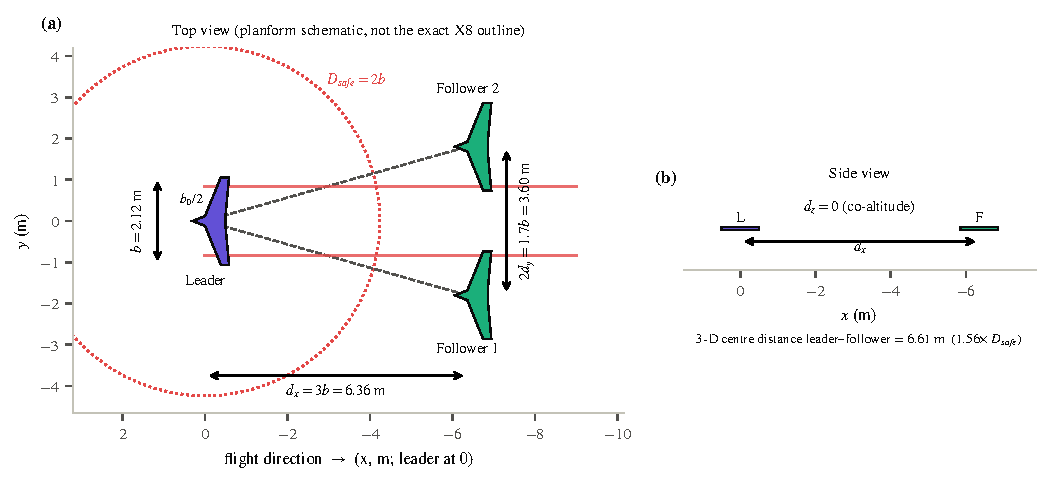
\includegraphics[width=\textwidth]{fig05_formation_geometry}
\caption{Three-UAV formation geometry (top and side views, nominal slot). The planform is a schematic, not the exact X8 outline.}\label{fig:geom}\end{figure}

\subsection{Guidance, NMPC and safety filter}
Each follower is a point-mass with first-order bank ($\tau_\phi=\SI{0.25}{s}$) and acceleration ($\tau_a=\SI{0.30}{s}$) lags, state $[p_x,p_y,V,\chi,\phi,a]$, inputs $[a_{\mathrm{cmd}},\phi_{\mathrm{cmd}}]$, ground velocity $V[\cos\chi,\sin\chi]+w_{\mathrm{eff}}$ with the wind low-pass filtered ($\tau_g$). A nonlinear MPC (multiple shooting, RK4, $N=25$, $\Delta t=\SI{0.1}{s}$, CasADi/IPOPT \cite{andersson2019,wachter2006}) tracks the slot position and velocity with quadratic cost and input-rate penalties and bank/speed/acceleration bounds. The wake-power term of the preliminary cost function is \emph{not} used here, so tracking and wake benefit are decoupled.

The safety layer enforces $h=\|p_f-p_L\|^2-D^2\ge0$ with $D=D_{\mathrm{safe}}+\SI{0.5}{m}$. Because bank enters through $\dot\phi=(\phi_{\mathrm{cmd}}-\phi)/\tau_\phi$ and acceleration through a lag, $h$ has \emph{relative degree 3} with respect to both inputs (the preliminary version stated 2). We therefore use a third-order HOCBF \cite{xiao2022,ames2017}: $\psi_0=h$, $\psi_{i}=\dot\psi_{i-1}+\alpha_i\psi_{i-1}$ ($\alpha=1.2,1.6,2.0$), constraint $\psi_3\ge0$ linear in the inputs, solved as a two-variable QP at \SI{50}{Hz} that minimally modifies the NMPC command. The filter is evaluated on a noisy relative-position measurement and, as shown in Sec.~\ref{sec:control}, it guarantees nothing when the constraint is infeasible within input limits.

\begin{algorithm}[H]
\caption{Supervisory logic per mission phase}\label{alg:sup}
\begin{algorithmic}[1]
\State \textbf{Takeoff/climb} individually; \textbf{join-up} to slot $(d_x,d_y)$ (Y=\SI{60}{m}), NMPC minimum-jerk reference
\State \textbf{Transit (formation)}: hold slot, rotate leader role cyclically (equalises battery drain)
\State \textbf{Split}: min-jerk lateral move to zone centre at planner-chosen peak lateral speed ($\le\SI{50}{\percent}$ of transit time)
\State \textbf{Map}: each UAV flies its own strips; early finishers loiter at best-endurance speed
\State \textbf{Merge}, formation transit home, \textbf{break-up}, landing
\State HOCBF filter active throughout; fall back to $d_y\ge 2.5b$ if relative-position uncertainty exceeds $0.5b$ (not exercised in the reported trials)
\end{algorithmic}\end{algorithm}

\subsection{Mission energy and coverage}
Energy is the integral of the power model over phases (climb, transit, mapping legs, Dubins turns, ferry legs, waiting, reconfiguration, landing) with wind-triangle ground speed on every leg. Turning between adjacent strips (spacing \SI{\ndyBase}{m} $<2R=\SI{141.7}{m}$) is a Dubins path with a straight run-in (\SI{441}{m} per turn, not the \SI{222.6}{m} semicircle of the preliminary version). Reconfiguration energy is \emph{simulated} (Sec.~\ref{sec:reconf}) rather than charged as full cruise power for an assumed duration. Coverage is a raster ray-multiplicity count of rotated rectangular footprints. A \SI{1}{ha} tile is \emph{geometrically accepted} if $\ge99\,\%$ is imaged and $\ge5$ images cover $\ge95\,\%$ of it. The RMSE criteria of the acceptance rule require SfM and were not evaluated.

\subsection{Formation guidance: NMPC formulation}\label{sec:nmpc}
Each follower is modelled as a point mass in the horizontal plane at constant altitude with state $\mathbf x=[p_x,p_y,V,\chi,\phi,a]^\top$ (north, east, airspeed, course, bank, along-track acceleration) and inputs $\mathbf u=[a_{\mathrm{cmd}},\phi_{\mathrm{cmd}}]^\top$:
\begin{equation}
\dot p_x=V\cos\chi+w_x,\;\dot p_y=V\sin\chi+w_y,\;\dot V=a,\;\dot\chi=\tfrac{g\tan\phi}{V},\;\dot\phi=\tfrac{\phi_{\mathrm{cmd}}-\phi}{\tau_\phi},\;\dot a=\tfrac{a_{\mathrm{cmd}}-a}{\tau_a},
\end{equation}
with $\tau_\phi=\SI{0.25}{s}$, $\tau_a=\SI{0.30}{s}$ and the aircraft's effective wind $\mathbf w_{\mathrm{eff}}$ a first-order lag ($\tau_g=\SI{1}{s}$) of the instantaneous wind, so that a sudden gust accelerates the aircraft over about a second instead of changing its ground velocity instantaneously. The wind consists of a common component (speed $U(2,6)$\,m/s, uniform direction), an individual Ornstein--Uhlenbeck component per aircraft ($\sigma=\SI{0.4}{m/s}$, correlation time \SI{2}{s}) and, in the gust scenarios, a differential lateral doublet applied to the follower only.

\paragraph{Optimal control problem} At \SI{10}{Hz} the NMPC solves, with multiple shooting, RK4 integration, $N=25$ steps of $\Delta t=\SI{0.1}{s}$,
\begin{equation}
\min_{\mathbf u_{0:N-1}}\ \sum_{k=0}^{N-1}\Big(\|\mathbf e_{p,k}\|^2_{Q_p}+\|\mathbf e_{v,k}\|^2_{Q_v}+\|\mathbf u_k\|^2_{R}+\|\mathbf u_k-\mathbf u_{k-1}\|^2_{R_d}\Big)+10\|\mathbf e_{p,N}\|^2_{Q_p}
\end{equation}
subject to the dynamics, $V\in[12,26]$\,m/s, $|\phi|\le35^\circ$, $|a|\le\SI{3}{m/s^2}$, $|a_{\mathrm{cmd}}|\le\SI{3}{m/s^2}$, $|\phi_{\mathrm{cmd}}|\le35^\circ$. Position and velocity references are the delayed, constant-velocity-extrapolated leader state plus the (minimum-jerk) slot trajectory; the wind estimate is a 1.5\,s lag of the true effective wind (an idealised observer). Weights: $Q_p=\mathrm{diag}(1,6)$, $Q_v=\mathrm{diag}(0.4,0.8)$, $R=\mathrm{diag}(0.2,3)$, $R_d=\mathrm{diag}(0.5,8)$ (the lateral channel is weighted more because the wake benefit lies within about $0.1b$). IPOPT \cite{wachter2006} is called through CasADi \cite{andersson2019} with a tolerance of $10^{-4}$, at most 60 iterations and warm starting; the wake term $w_{\mathrm{wake}}\Delta P$ of the preliminary cost is not used. The baseline controller is a PD law in the follower-heading frame ($a_x=0.30e_x+0.9\dot e_x$, $a_y=0.45e_y+1.1\dot e_y$, $\phi_{\mathrm{cmd}}=\arctan(a_y/g)$) with the same limits.

\subsection{High-order barrier-function safety filter}\label{sec:hocbf}
Let $\mathbf r=\mathbf p_f-\mathbf p_L$ and $h(\mathbf x)=\|\mathbf r\|^2-D^2\ge0$ with $D=D_{\mathrm{safe}}+\SI{0.5}{m}$. Differentiating along the follower dynamics, $\dot h=2\mathbf r\cdot\dot{\mathbf r}$ contains no input; $\ddot h=2\|\dot{\mathbf r}\|^2+2\mathbf r\cdot\ddot{\mathbf r}$ contains the acceleration state $a$ and the bank state $\phi$ (through $\dot\chi$) but not $a_{\mathrm{cmd}}$ or $\phi_{\mathrm{cmd}}$; only the third derivative contains the commands, through $\dot a=(a_{\mathrm{cmd}}-a)/\tau_a$ and $\dot\phi=(\phi_{\mathrm{cmd}}-\phi)/\tau_\phi$. The relative degree is therefore $3$ for both inputs (the preliminary version stated 2, which holds only if bank and acceleration are directly commanded). Following \cite{xiao2022} define
\begin{equation}
\psi_0=h,\qquad \psi_i=\dot\psi_{i-1}+\alpha_i\psi_{i-1}\ (i=1,2,3),\qquad (\alpha_1,\alpha_2,\alpha_3)=(1.2,1.6,2.0),
\end{equation}
so that $\psi_3\ge0$ is affine in $\mathbf u$ and renders the set $\{h\ge0\}$ forward invariant \emph{provided} the constraint is feasible within the input bounds. The filter solves at \SI{50}{Hz}
\begin{equation}
\mathbf u^\star=\arg\min_{\mathbf u\in\mathcal U}\tfrac12\|\mathbf u-\mathbf u_{\mathrm{nom}}\|^2\quad\text{s.t.}\quad \mathbf A(\mathbf x)\mathbf u+c(\mathbf x)\ge0,
\end{equation}
where $\mathbf A,c$ are generated symbolically by CasADi from the composition above, using the noisy measured relative position. The QP has two unknowns and one affine constraint over the input box $\mathcal U=[-3,3]\,\mathrm{m/s^2}\times[-35^\circ,35^\circ]$ and is solved by SLSQP in about a millisecond (when the affine barrier half-space conflicts with $\mathcal U$, SLSQP terminates at the box-boundary point minimising constraint violation and clips to $\mathcal U$, rather than introducing an explicit slack variable). Although the filter's internal Lie derivatives include the nominal first-order actuator lags $(\tau_\phi,\tau_a)$ to reach relative degree $3$, the continuous-time forward-invariance guarantee still does not carry over to the closed-loop simulation because of (i) hard input saturation on $\mathcal U$, (ii) unmodelled leader deceleration $\dot{\mathbf v}_L\ne\mathbf 0$ and communication dropouts (the filter differentiates under a constant-velocity leader assumption), (iii) unsteady wind gusts, the effective-wind lag $\tau_g$ and the \SI{1.5}{s} wind-observer lag, (iv) discrete-time \SI{50}{Hz} sampling and the \SI{12}{m/s} airspeed floor, and (v) relative-position measurement noise and GNSS bias. Furthermore, because $h$ is purely radial with fixed class-$\mathcal K$ gains, $\nabla h$ at $(d_x=-3b,d_y=0.85b)$ is predominantly longitudinal, so the myopic single-step QP saturates longitudinal braking before initiating an early lateral break-away manoeuvre of the kind synthesized by backup or adaptive CBFs \cite{chen2021backup,xiao2021ada,molnar2025}; Sec.~\ref{sec:control} therefore reports empirical violation rates rather than a proof.

\subsection{Reconfiguration manoeuvres}\label{sec:reconfdesign}
A \emph{split} moves each follower laterally from its V slot to the centre of its survey zone ($Y=\SI{369.6}{m}$ for the 17-strip plan, \SI{370}{m} for the 14-strip plan; \SI{60}{m} for join-up after take-off and break-up before landing). The lateral reference is a minimum-jerk profile $y(t)=y_0+(y_1-y_0)(10s^3-15s^4+6s^5)$, $s=(t-t_0)/T$, with duration $T=1.875\,Y/v_{\mathrm{lat}}$ for a peak lateral speed $v_{\mathrm{lat}}$ chosen from $\{3,4,6,8,12\}$\,m/s; the NMPC tracks it while keeping the along-track position, so the follower flies a longer path at a higher airspeed (to hold ground speed) and loses the wake benefit as it leaves the slot. The planner selects, for each manoeuvre, the speed that minimises the follower's energy relative to staying in formation, subject to the window using at most half of a one-way transit. Energy over the window is integrated with the full power model using the simulated airspeed, bank and slot offset (the wake term is interpolated from the aerodynamic table), so the cost of a manoeuvre is a simulation output rather than an assumed duration.

\subsection{Mission accounting}\label{sec:accounting}
For each aircraft the mission is a sequence of phases $j$ with power $P_j$ and duration $t_j$; the load-side energy is $E=\sum_jP_jt_j/3600$ and the cell-side energy follows from the battery model. Phases: (i) climb to \SI{120}{m} at \SI{2}{m/s} ($P=P_{\mathrm{cruise}}+mg\,\mathrm{ROC}/\eta_p$); (ii) outbound transit of length $D$ (hypotenuse to the zone for independent aircraft), with the wind-triangle ground speed; (iii) strip legs of \SI{1}{km}; (iv) Dubins turns of length $L_t$ at the turn power; (v) a ferry leg of \SI{1}{km} for an aircraft that ends its last strip on the far side of the polygon; (vi) waiting at the best-endurance speed (\SI{\nnPwait}{W}) until the slowest aircraft finishes, only for strategies that must re-form; (vii) reconfiguration windows; (viii) return transit; (ix) \SI{90}{s} of approach and landing at cruise power. In formation transit the leader role rotates, so each aircraft pays the mean of the leader and follower power, $P_{\mathrm{form}}=(P_{\mathrm{iso}}+2P_{\mathrm{fol}})/3$, with $P_{\mathrm{fol}}$ computed from the drag reduction at the realised slot error (sampled from the control campaign). A rigid V flies the whole 17-strip block with the followers' turn speeds $\Va(1\pm d_y/R_t)$ and no wake benefit in turns. Strip counts per aircraft are $(6,6,5)$ for the 17-strip plan and $(5,5,4)$ for the 14-strip plan.

\subsection{Coverage and acceptance rule}\label{sec:acceptance}
Ground footprints are rectangles $W_g\times H_g$ rotated by the crab angle, triggered every $H_g(1-o_f)$ along track, starting and ending half a footprint outside the polygon. The number of images covering each $\SI{2}{m}$ raster cell is accumulated. A \SI{1}{ha} tile is accepted if at least \SI{99}{\percent} of its cells are covered and at least \SI{95}{\percent} are covered by $\ge5$ images; the preliminary version's additional criteria on checkpoint RMSE \cite{asprs2024} are \emph{not} evaluated here. Strip centres are placed symmetrically; the \SI{58}{\percent} plan is evaluated both with its nominal spacing (\SI{73.92}{m}) and with the smallest spacing that meets the five-ray rule at the block edge (\SI{74.0}{m}).


%==============================================================================================
\section{Methods and verification}\label{sec:methods}
\paragraph{Experimental unit and pairing} One \emph{trial} is one environment realisation: wind speed $U(2,6)$\,m/s, direction $U(0,2\pi)$, and one recorded \SI{40}{s} follower station-keeping error series bootstrapped from the control campaign (so aerodynamic benefit reflects realised, not ideal, slot keeping). Every strategy and aerodynamic model is evaluated on the same realisation; paired differences are the outcomes. $\nnTrials$ trials were run (seed 20260101).

\paragraph{Aerodynamic model ensemble} Because the wake model is the dominant epistemic uncertainty, every mission result is computed with five aerodynamic variants: the manuscript's equations as published (audit only), corrected strip theory, VLM with a rolled-up pair, VLM with the planar sheet (reported as headline: it has an independent verification and is the upper bound) and VLM in the free wake (finite cores; the more conservative bound). Spread among them is the model-form uncertainty.

\paragraph{Control campaign} Six scenarios $\times$ three controllers (PD baseline, NMPC, NMPC+HOCBF) $\times$ 30 seeds (\nnControl{} runs; same seed $=$ same disturbance): turbulence, \SI{8.5}{m/s} differential gust doublet, \SI{4}{m/s} leader braking with \SI{250}{ms} dropout, degraded GNSS (\SI{0.5}{m} noise, \SI{1.5}{m} bias), their combination, and a deliberately over-capability \SI{6}{m/s} braking in \SI{1.5}{s}. The NMPC solved in \SI{\nsolveMean}{ms} on average (maximum \SI{\nsolveMax}{ms}) with no solver failures.

\paragraph{Statistics} For paired outcomes we report mean differences and the 5--95\,\% range of trial-wise relative differences. Because the simulator is nearly deterministic given the environment, paired differences have tiny variance and conventional $p$-values and Cohen's $d_z$ (here $|d_z|$ up to \ndzA--\ndzC) are mathematically large but carry \emph{no} evidential weight about real aircraft; we therefore do not use hypothesis tests as support. Holm-adjusted $p$-values \cite{holm1979}, bootstrap intervals \cite{efron1993} and Wilcoxon statistics are in the archived tables for completeness. Global sensitivity uses standardised regression coefficients \cite{saltelli2008}.

\paragraph{Reproducibility} All figures and every number in this paper are generated by scripts from raw CSV/NPZ files (\texttt{make reproduce}); unit tests cover the closed-form checks in Sec.~\ref{sec:model} and the audit findings of \ref{app:audit}.

%==============================================================================================
\section{Results}
\subsection{Aerodynamic interaction}\label{sec:aero}
\begin{figure}[H]\centering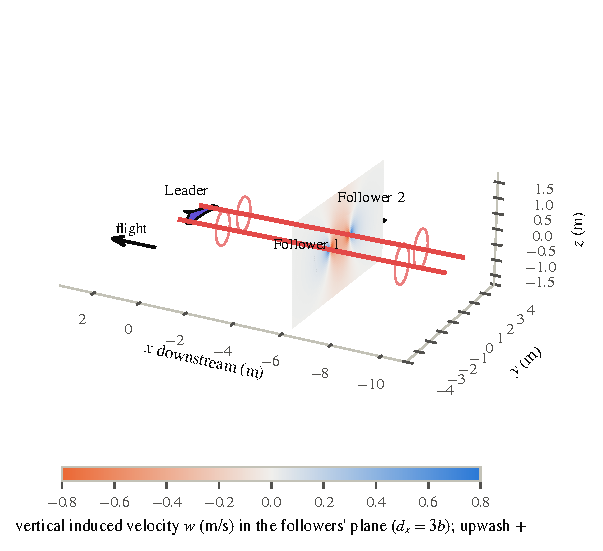
\includegraphics[width=0.95\textwidth]{fig01_wake_3d}
\caption{Wingtip-vortex pair (red) and vertical induced velocity at the followers' plane ($d_x=3b$) for the nominal geometry; analytic Lamb--Oseen field with corrected $\Gamma_0$.}\label{fig:wake3d}\end{figure}
\begin{figure}[H]\centering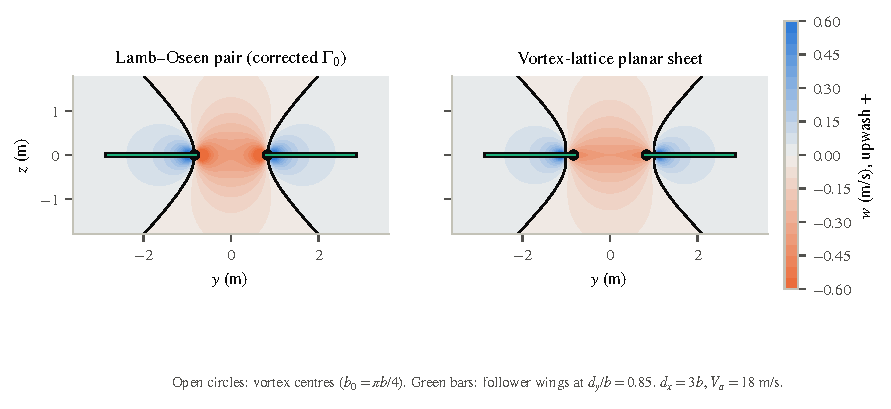
\includegraphics[width=\textwidth]{fig02_wake_contours}
\caption{Vertical induced velocity $w(y,z)$ behind the leader at $d_x=3b$: analytic pair (left) and vortex-lattice planar sheet (right). Upwash $>0$ outboard of the vortex centres.}\label{fig:wakecont}\end{figure}

Figures~\ref{fig:wake3d}--\ref{fig:wakecont} show the geometry and the field. With the corrected circulation, the corrected strip model and the vortex-lattice variants agree on the shape of the benefit (Fig.~\ref{fig:A2}): a broad maximum of \npeakFree--\npeakSheet\,\% follower electrical-power saving at $d_y/b\approx0.85$--$0.90$ (\npeakFree\,\% free wake, \npeakStrip\,\% corrected strip, \npeakRolled\,\% rolled-up pair, \npeakSheet\,\% planar sheet), decaying slowly outboard. At the preliminary version's slot, $d_y=0.8b$, the saving is \natEightyStrip\,\% (strip, corrected) to \natEightySheet\,\% (VLM sheet), against \npubAtEighty\,\% as published. The published equations place a sharp peak at exactly $0.80b$ with a \npubAtEightyFive\,\% saving at $0.85b$ and a \npubDropNinety\,\% loss at $0.90b$; \ref{app:audit} shows this feature is an artefact of the two errors above, which cancel only near $0.80b$ and are not reproduced by the published table itself.

\begin{figure}[H]\centering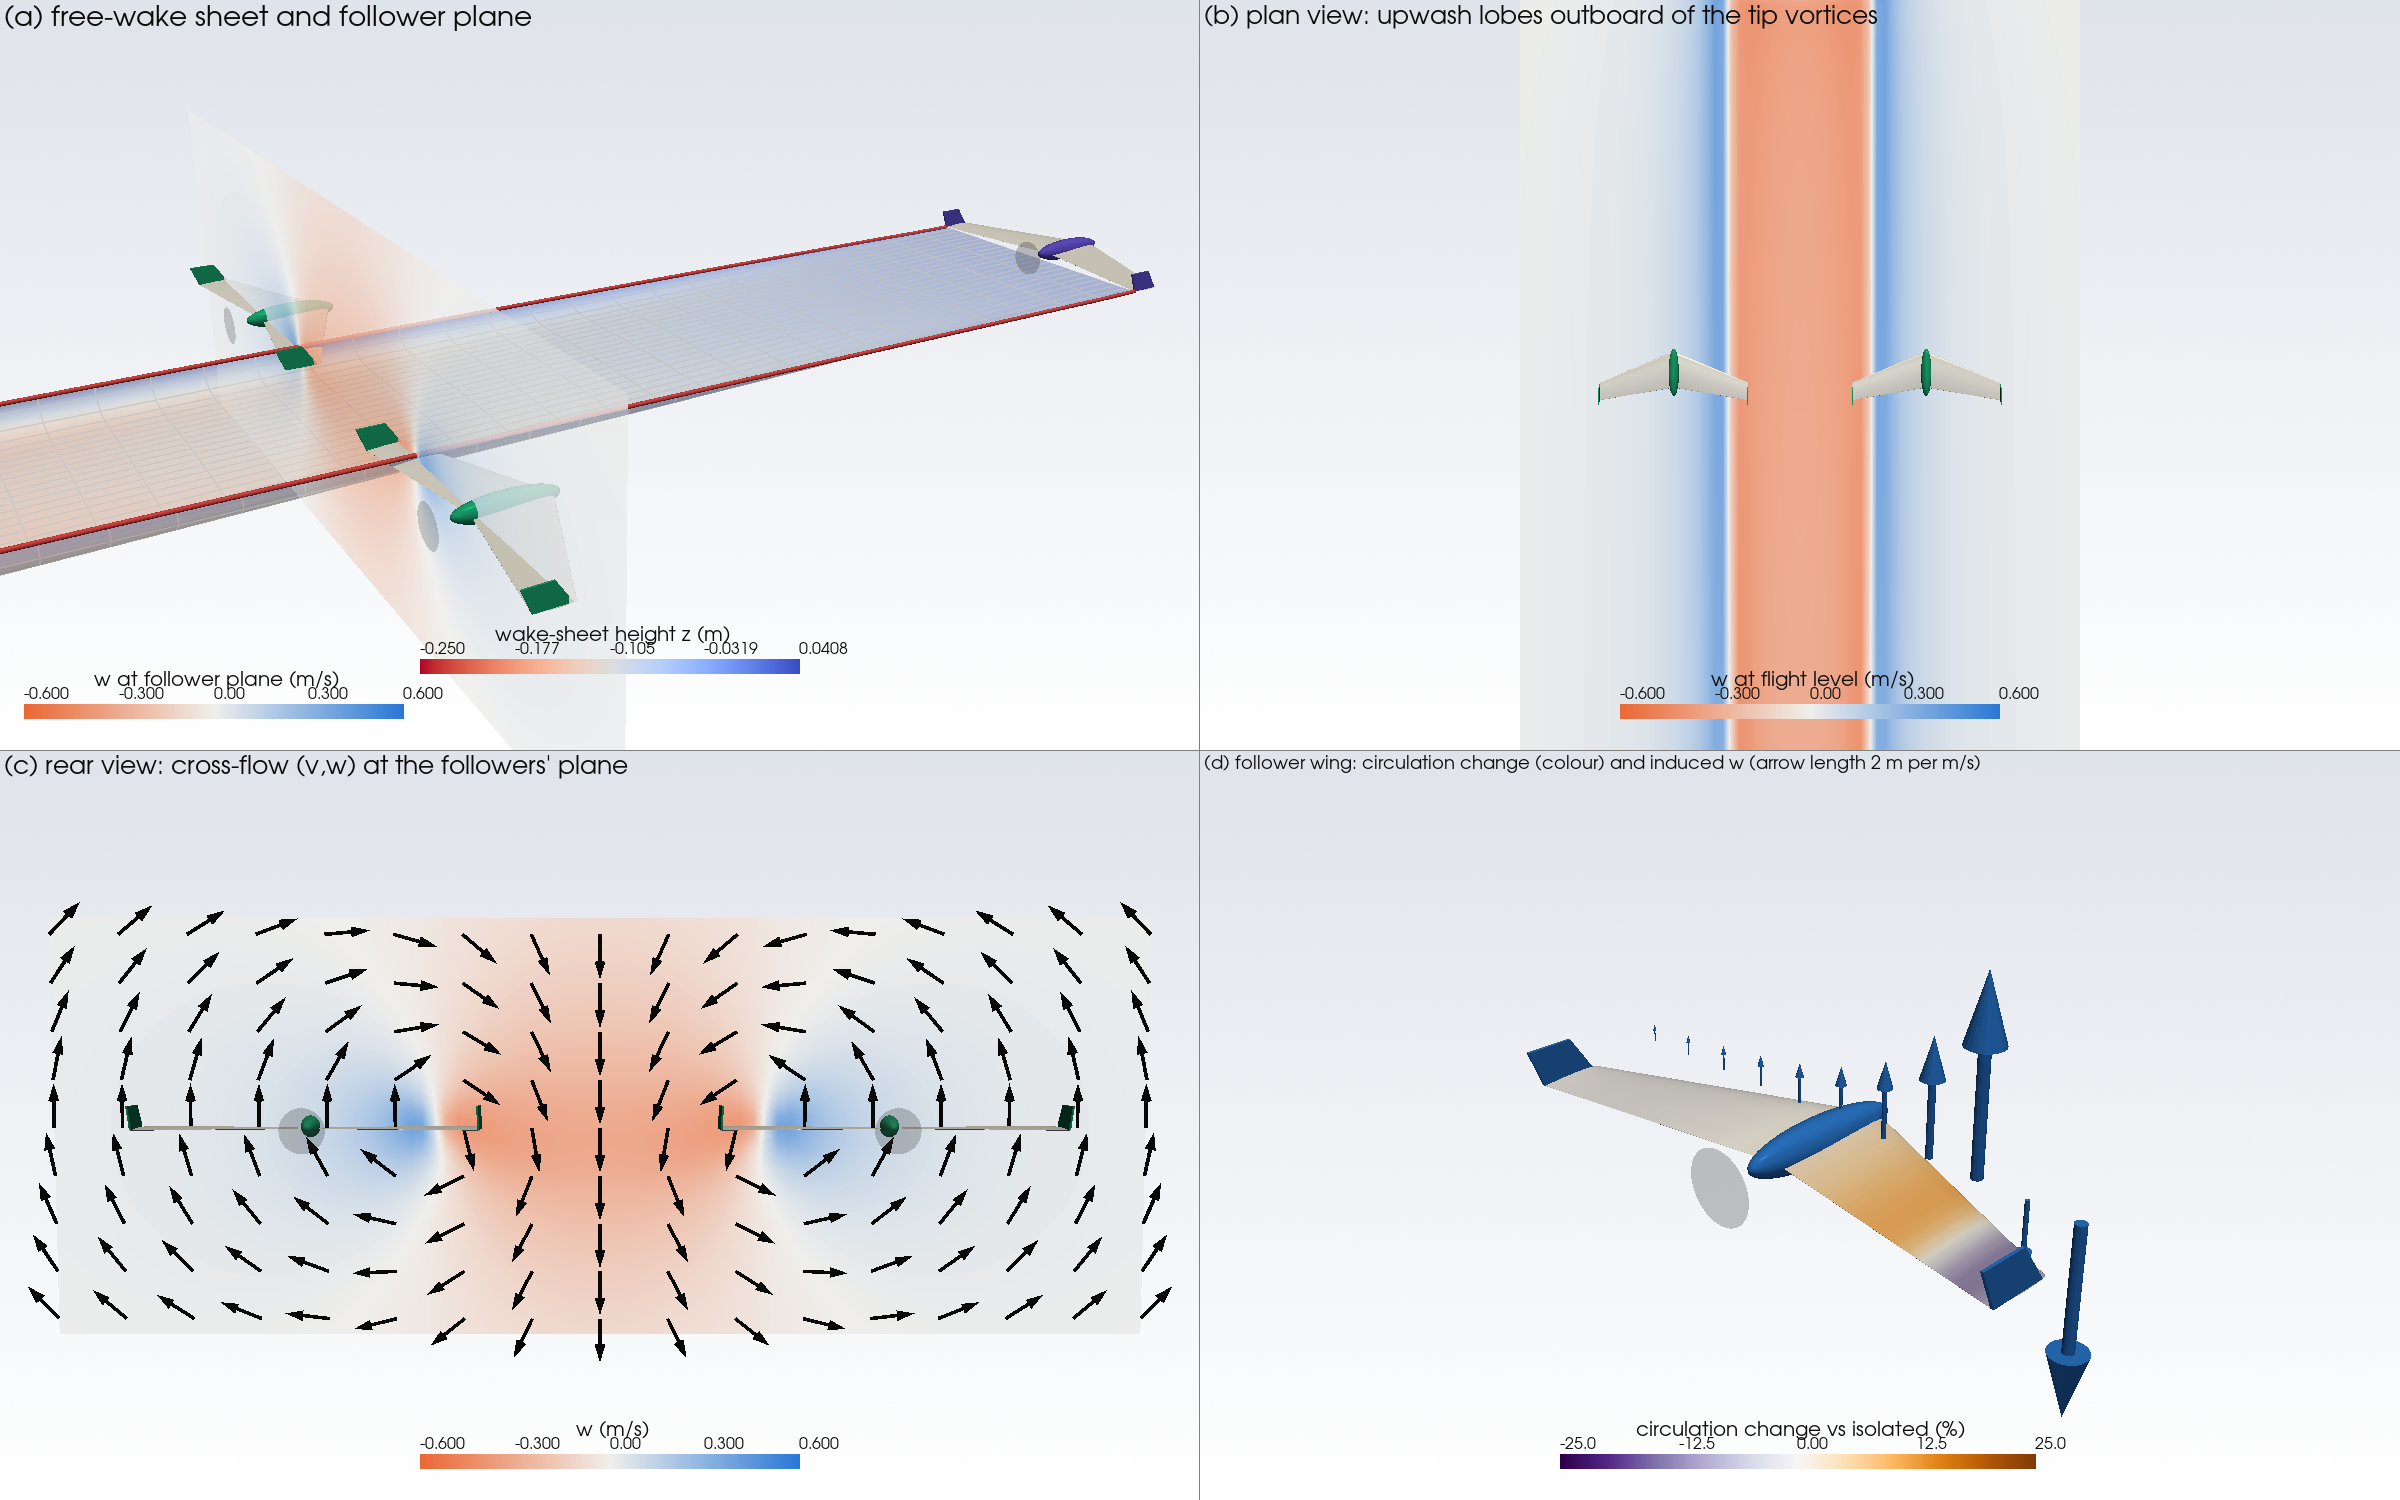
\includegraphics[width=\textwidth]{A1_freewake_formation}
\caption{Three-dimensional free-wake simulation of the formation ($d_x=3b$, $d_y=0.85b$; real-scale X8-class meshes). (a) Wake sheet, coloured by height, and the induced vertical velocity at the followers' plane; (b) plan view of the vertical velocity at flight level: upwash lobes lie outboard of the tip vortices, the downwash trough between them; (c) cross-flow vectors $(v,w)$ at the followers' plane; (d) follower wing coloured by the circulation change relative to isolated flight, with the induced upwash along the span.}\label{fig:A1fw}\end{figure}
\begin{figure}[H]\centering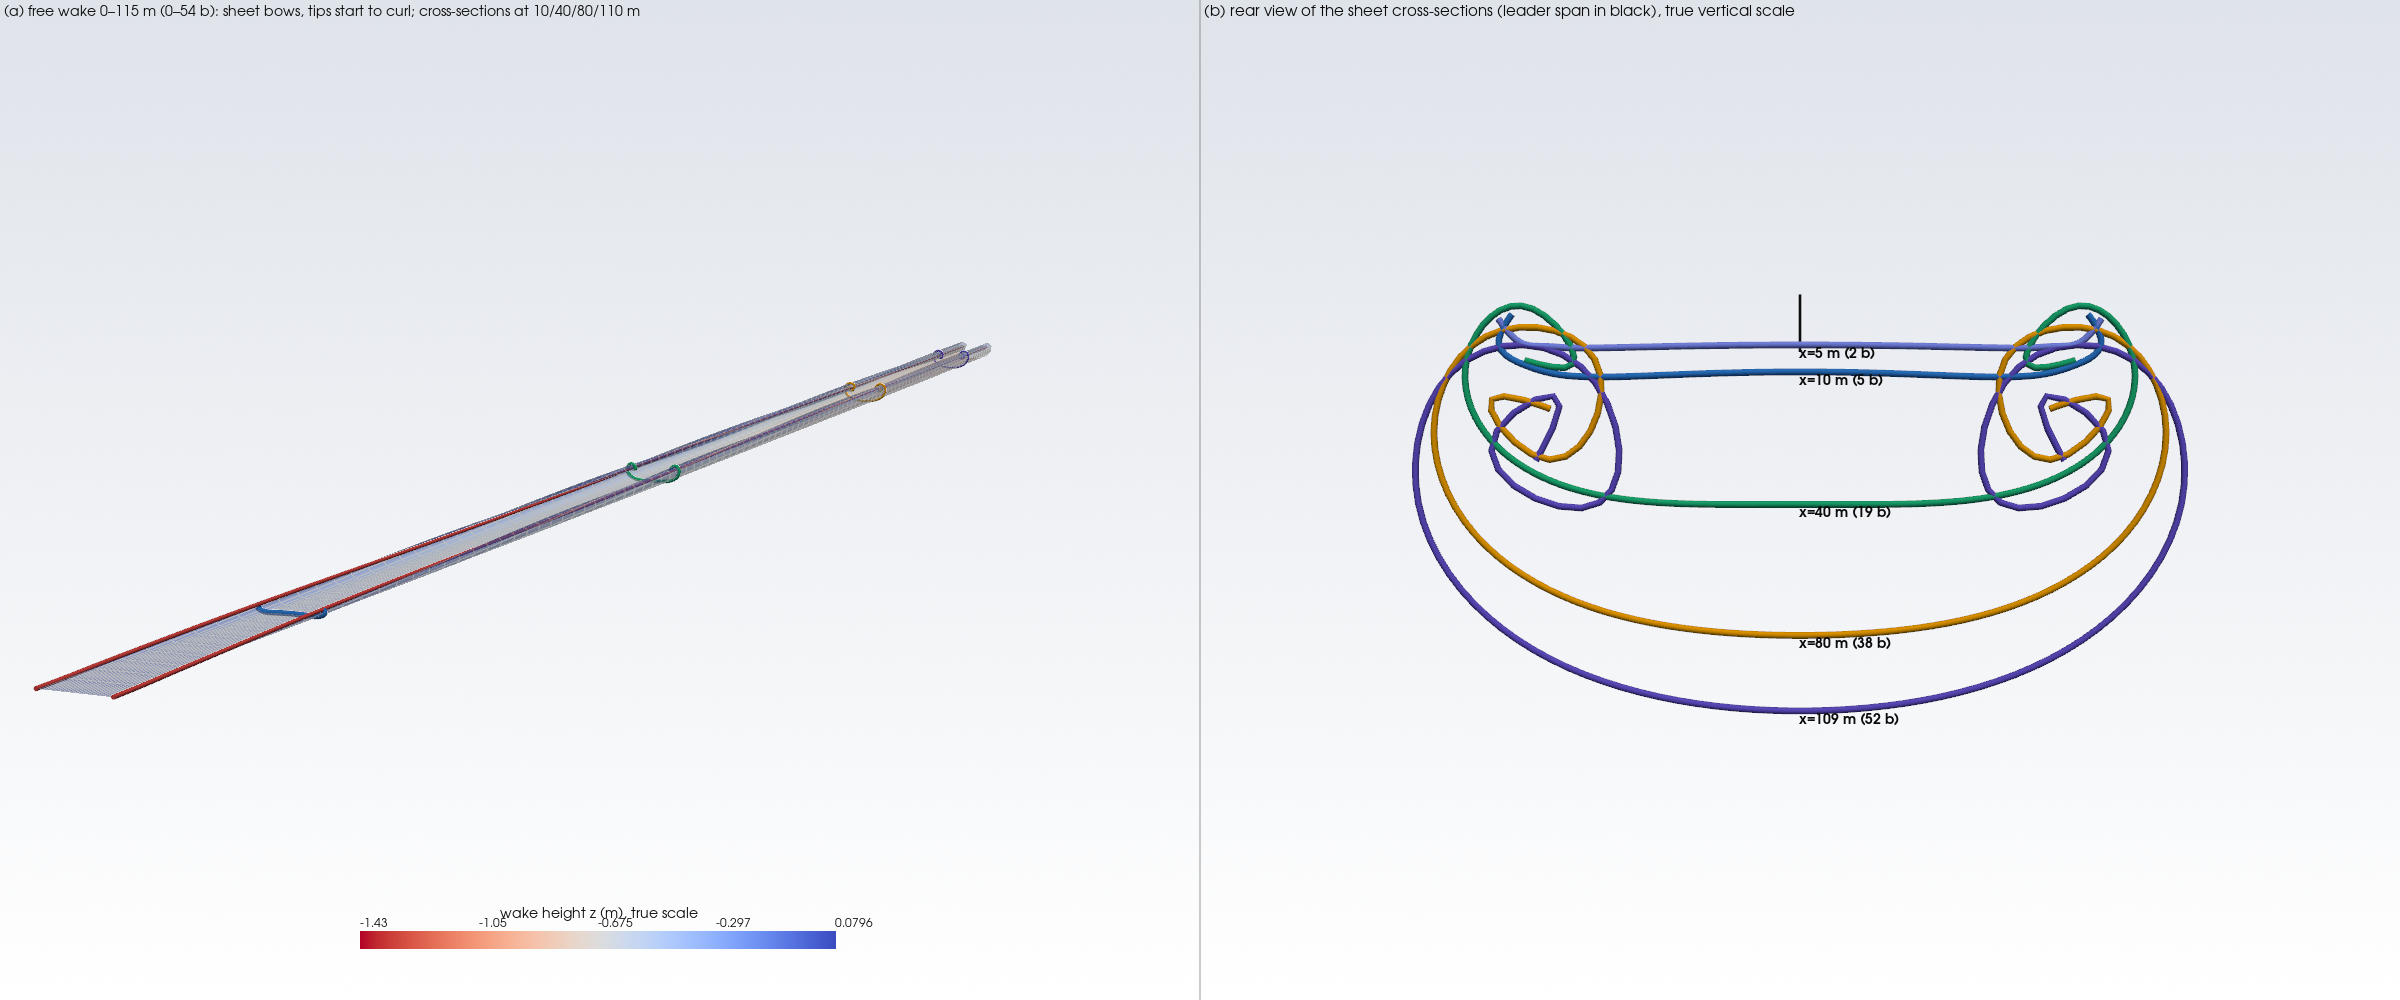
\includegraphics[width=\textwidth]{A2_wake_rollup}
\caption{Long free-wake run (\nfwXend{} m, $\nfwXendB\,b$). (a) The sheet at true scale; coloured cross-sections at 10, 40, 80 and 110 m. (b) The same cross-sections seen from behind at true vertical scale: the centre sinks \nfwCentreZ{} m while the tips sink \nfwTipZ{} m and begin to curl into spirals, but no coherent vortex pair has formed.}\label{fig:A2roll}\end{figure}
\begin{figure}[H]\centering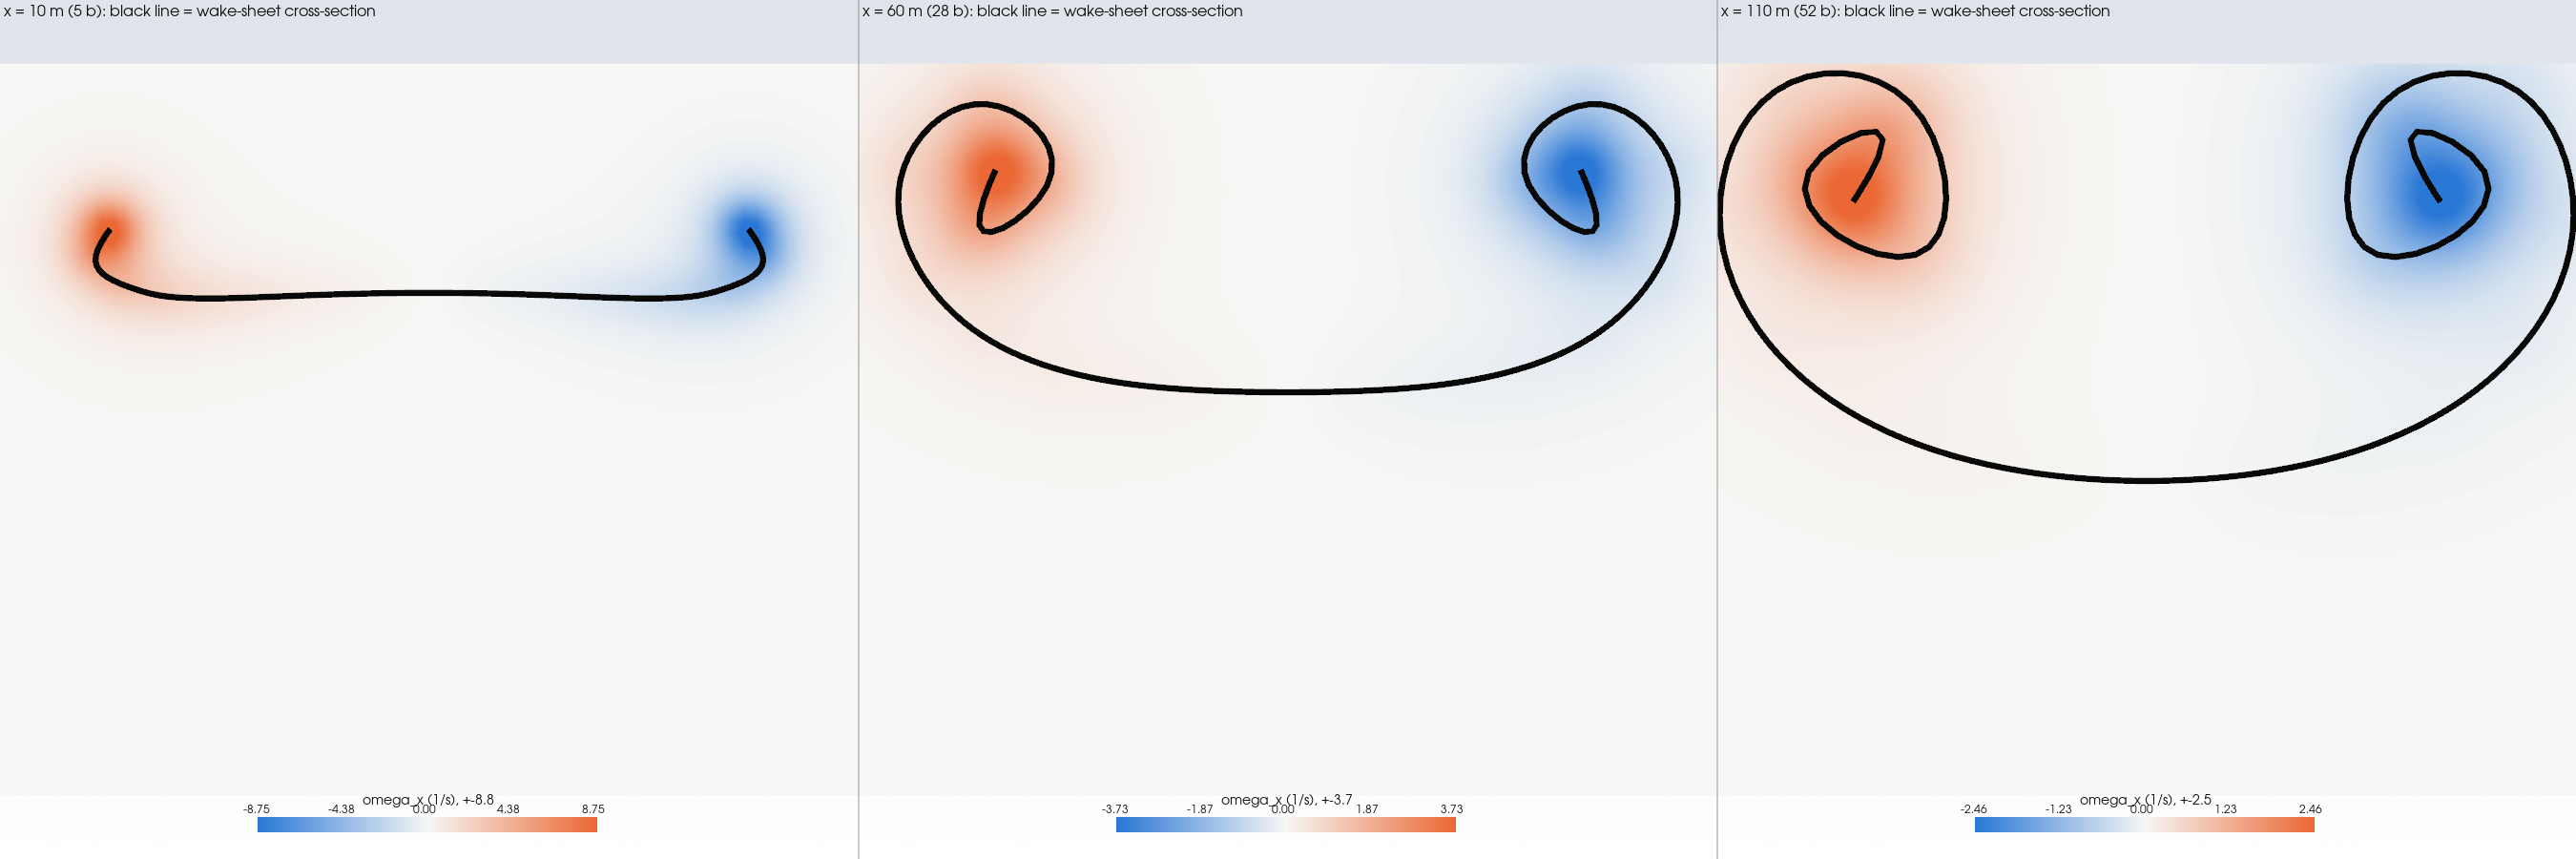
\includegraphics[width=\textwidth]{A3_vorticity_isosurface}
\caption{Streamwise vorticity $\omega_x=\partial w/\partial y-\partial v/\partial z$ on cross-flow planes following the sinking sheet at 10, 60 and 110 m behind the leader (free-wake field).}\label{fig:A3vort}\end{figure}
\begin{figure}[H]\centering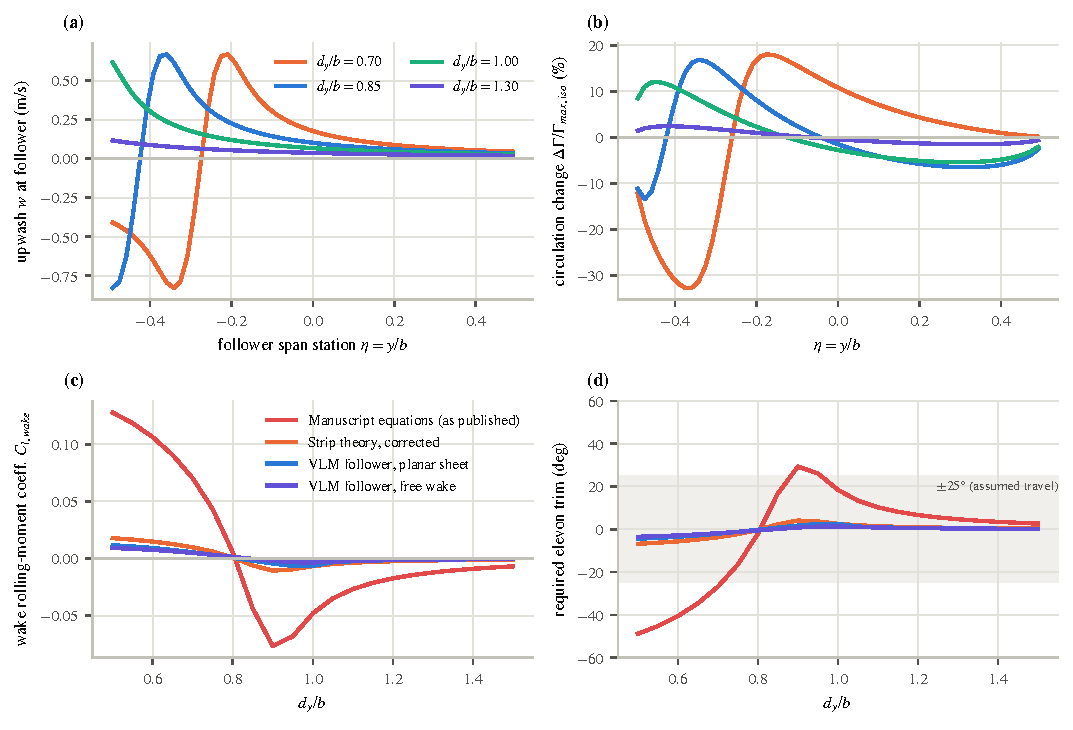
\includegraphics[width=\textwidth]{fig03_spanwise_loading}
\caption{Follower response: (a) upwash across the span and (b) circulation change from the VLM follower in the rolled-up (finite-core) wake (the planar sheet has line-vortex singularities at the tip-vortex crossing that make local values spiky, although integrated forces stay finite), (c) wake rolling-moment coefficient and (d) elevon deflection required to trim, for the three analyses. The published equations demand implausible elevon angles away from $0.8b$.}\label{fig:loading}\end{figure}

The free wake adds two facts the idealised models could not. First, at the formation distance the sheet is bowed but not rolled up (centre-to-tip sag \nfwSagTen\,cm at \SI{10}{m} and \nfwSagForty\,m at \SI{40}{m}); tips begin to curl at roughly 20--40 spans and no coherent pair exists even at $\nfwXendB\,b$ (Figs.~\ref{fig:A2roll}--\ref{fig:A3vort}). The assumption of a fully rolled-up Lamb--Oseen pair at $3b$ in the preliminary version is therefore not supported; the planar sheet and free wake are the appropriate near-wake descriptions. Second, with finite cores the follower sees less upwash than from the singular line-vortex tips of the planar sheet: the saving at $0.9b$ is \npeakFree\,\% (free wake) against \npeakSheet\,\% (sheet), and varies from \ncoreBig\,\% to \ncoreSmall\,\% as the core radius goes from $0.10b$ to $0.02b$ (\ncoreLo--\ncoreHi\,\% over the runs tested). The core radius is not calibrated, so the free-wake figure is a plausible lower bound and the sheet an upper bound.

Spanwise loading (Fig.~\ref{fig:loading}) shows why trim matters less than the preliminary version claimed: with the dimensionally consistent coefficient, $|C_{l,\mathrm{wake}}|$ stays below 0.02 over the offsets of interest, trim angles remain a few degrees and trim drag is negligible compared with the induced-drag change.

\begin{figure}[H]\centering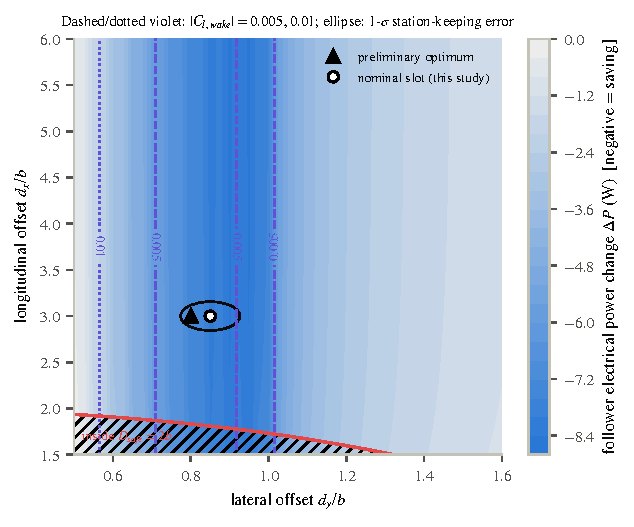
\includegraphics[width=0.75\textwidth]{fig04_sensitivity_map}
\caption{Follower power change over longitudinal and lateral offset (VLM planar sheet, $\Va=\SI{18}{m/s}$). Hatched: inside $D_{\mathrm{safe}}$. Ellipse: $1\sigma$ station-keeping error from the control campaign (scenario S1, NMPC+HOCBF). A planar sheet has no roll-up or decay, so the weak $d_x$ dependence is a model limitation, not a result.}\label{fig:map}\end{figure}

The benefit region is wide in $d_y$ (Fig.~\ref{fig:map}); the station-keeping error of the NMPC (RMS $e_y=\SI{\nrmsEySOneC}{m}$, $\nrmsEyFracB\,b$) is small relative to it, and the realised mean follower saving in the mission simulation was \nsavFrac\,\%. The maximum modelled saving is \nmapMinW\,W per follower (about 6\,\% of \SI{\npIso}{W}). The saving scales steeply with airspeed (Fig.~\ref{fig:sens}a): with the VLM sheet it is \nsheetVThirteen\,\% at \SI{13}{m/s}, \nsheetVEighteen\,\% at \SI{18}{m/s} and \nsheetVTwentyFour\,\% at \SI{24}{m/s}. The 5--95\,\% band from parametric uncertainty (drag, efficiency, hotel load, viscosity, core size, circulation $\pm15$\,\%, position error) around corrected strip theory at \SI{18}{m/s} is \nuncEighteenLo--\nuncEighteenHi\,\%; this band reflects parameter uncertainty only and does not include the unquantified roll-up/decay error that CFD would resolve.

\subsubsection{Vertical offset}
All results so far assume co-altitude flight. Figure~\ref{fig:X1} adds the vertical offset $d_z$: the benefit is concentrated in a narrow band around the wake sheet. At $d_y=0.85b$ the saving halves at $|d_z|\approx\ndzHalfFree\,b$ (\SI{\ndzHalfM}{m}) for the free wake and $\ndzHalfSheet\,b$ for the planar sheet; at $d_z=0.2b$ it is \ndzAtPtTwoFree\,\% (free) and \ndzAtPtTwoSheet\,\% (sheet) and at $0.4b$ only \ndzAtPtFourFree\,\% and \ndzAtPtFourSheet\,\%, against peaks of \ndzPeakFree\,\% and \ndzPeakSheet\,\%. The vertical station-keeping requirement, roughly $\pm0.1b$ ($\pm\SI{0.2}{m}$), is therefore as demanding as the lateral one, and altitude hold of small UAVs (barometer and GNSS noise of the order of decimetres) is a practical limit that the 2-D guidance model does not represent. Both models place the contour of zero benefit at $d_y\approx0.55$--$0.6b$ at $d_z=0$, and the zero contour widens with $|d_z|$: a follower that is far above or below the wake never gains, but it also never suffers the downwash penalty.
\begin{figure}[H]\centering\includegraphics[width=\textwidth]{X1_vertical_offset}
\caption{Follower electrical-power saving over lateral and vertical offset ($d_x=3b$, $\Va=\SI{18}{m/s}$) for (a) the planar sheet and (b) the free wake; (c) vertical cut at $d_y=0.85b$. Black: zero-saving contour; dot: nominal slot.}\label{fig:X1}\end{figure}

\subsubsection{Station-keeping accuracy}
The saving realised in flight is the expectation of the static saving over the slot error. Convolving the Gaussian lateral error distribution $\mathcal N(0,\sigma_y^2)$ with the static saving curve (evaluated on the Cauchy-midpoint lattice $d_y/b=m/60$ via 61-point Gauss--Hermite quadrature so collocation points never land on singular trailing filaments; Fig.~\ref{fig:X4}) shows how fast accuracy is lost: at $d_y=0.85b$ the VLM-sheet saving falls monotonically from \nskZeroSheet\,\% to \nskFifteenSheet\,\% at $\sigma_y=\SI{0.15}{m}$ (the NMPC's RMS error in turbulence), i.e.\ \nskRetain\,\% of the ideal value is retained, to \nskFortyKSheet\,\% at \SI{0.4}{m} and to \nskSixtySheet\,\% at \SI{0.6}{m}. The free-wake and strip models behave alike (\nskZeroFree\,\% $\to$ \nskFifteenFree\,\% $\to$ \nskFortyKFree\,\% and \nskZeroStrip\,\% $\to$ \nskFifteenStrip\,\% $\to$ \nskFortyKStrip\,\%). With GNSS-only relative navigation (error of order \SI{1}{m}) the expected benefit is negligible, which is the quantitative reason that the supervisor widens the lateral spacing when the relative-position uncertainty grows (Alg.~\ref{alg:sup}).
\begin{figure}[H]\centering\includegraphics[width=\textwidth]{X4_station_keeping_error}
\caption{Expected follower electrical-power saving versus lateral station-keeping error $\sigma_y$ (Gauss--Hermite quadrature over the Cauchy-midpoint static saving curve). (a) Three aerodynamic models at $d_y=0.85b$; (b) three nominal slots for the VLM planar sheet.}\label{fig:X4}\end{figure}

\subsubsection{Power curve and the choice of cruise speed}
Figure~\ref{fig:X6} places the wake benefit in the context of the aircraft's power curve. Electrical power is minimal at \SI{\npowMinV}{m/s} (\SI{\npowMinP}{W}) and energy per kilometre at \SI{\npowRangeV}{m/s} (\SI{\npowRangeE}{Wh/km}); the nominal \SI{18}{m/s} costs \SI{\npowEOneEight}{Wh/km}, only \npowExcess\,\% above the best-range value, so formation transit at a lower speed would not be competitive with simply cruising at the best-range speed unless the wake saving exceeds that margin. The percentage saving rises steeply as speed falls (induced-drag share grows), reaching \nsheetVThirteen\,\% (sheet) at \SI{13}{m/s}; in absolute terms, however, the power a follower can shed is at most about \SI{9}{W} at any speed, which is why the benefit cannot compete with the fixed overheads of reconfiguration unless the transit is long.
\begin{figure}[H]\centering\includegraphics[width=\textwidth]{X6_power_curve}
\caption{(a) Isolated electrical and aerodynamic power versus airspeed with the minimum-power point; (b) energy per kilometre and best-range speed; (c) follower saving at $d_y=0.85b$ versus airspeed for three wake models.}\label{fig:X6}\end{figure}


\subsection{Controller performance and safety}\label{sec:control}
\begin{figure}[H]\centering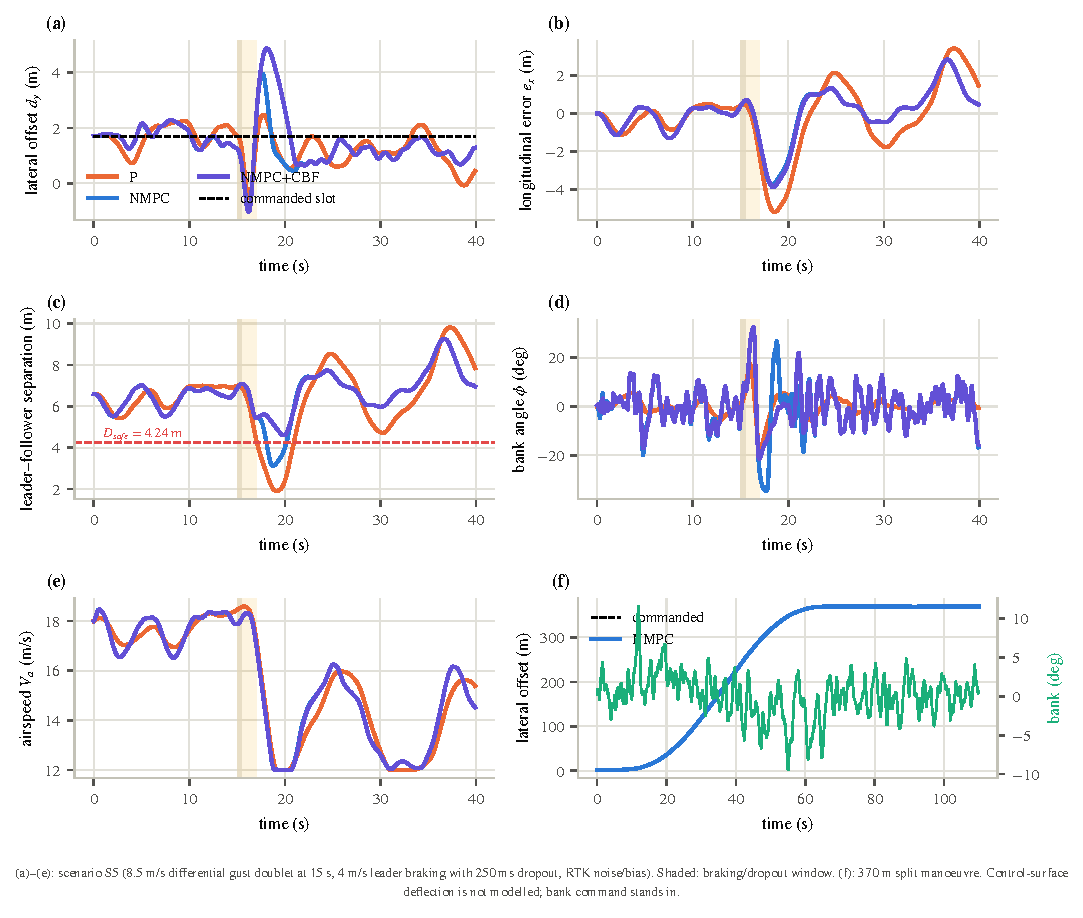
\includegraphics[width=\textwidth]{fig07_control_performance}
\caption{Scenario S5 (combined disturbance) for one seed, the three controllers, and a \SI{370}{m} split manoeuvre (f). Panel (a): lateral offset; (c): separation vs.\ $D_{\mathrm{safe}}$; (e): airspeed floor at \SI{12}{m/s} is reached while closing on a braking leader.}\label{fig:ctrl}\end{figure}
\begin{figure}[H]\centering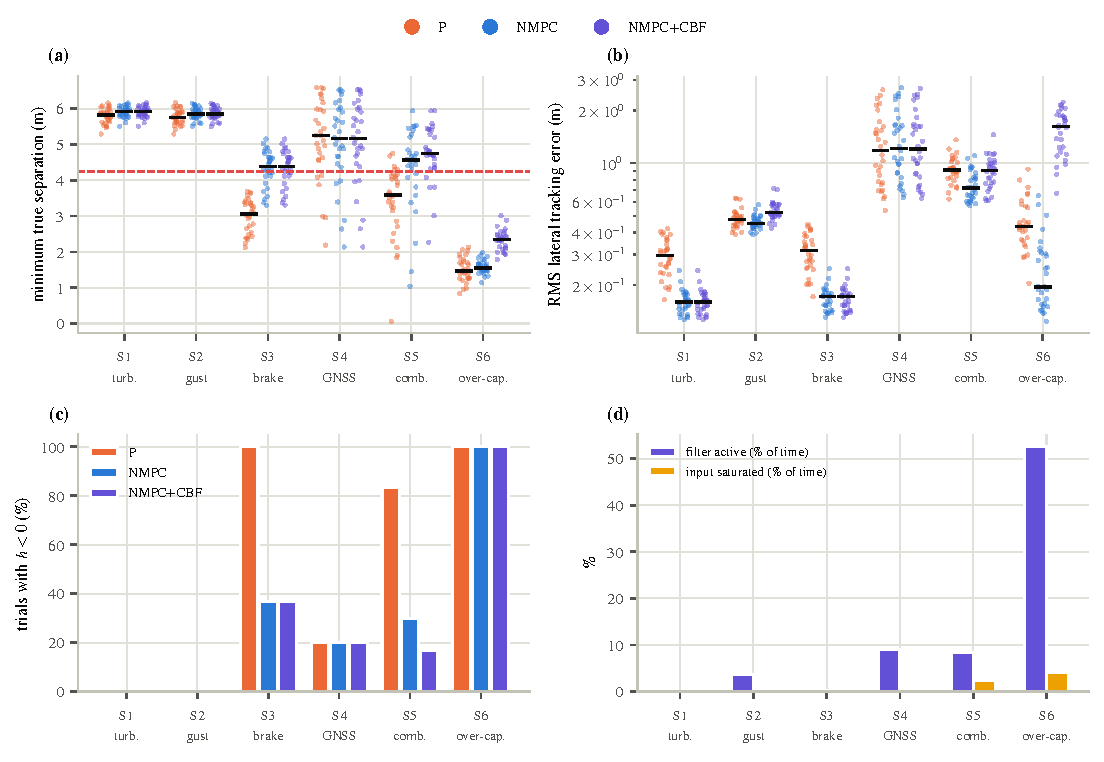
\includegraphics[width=\textwidth]{fig14_safety_tracking}
\caption{All \nnControl{} control runs: (a) minimum true separation, (b) RMS lateral error, (c) fraction of trials entering the unsafe set ($h<0$), (d) HOCBF activity and input saturation.}\label{fig:safety}\end{figure}
\begin{figure}[H]\centering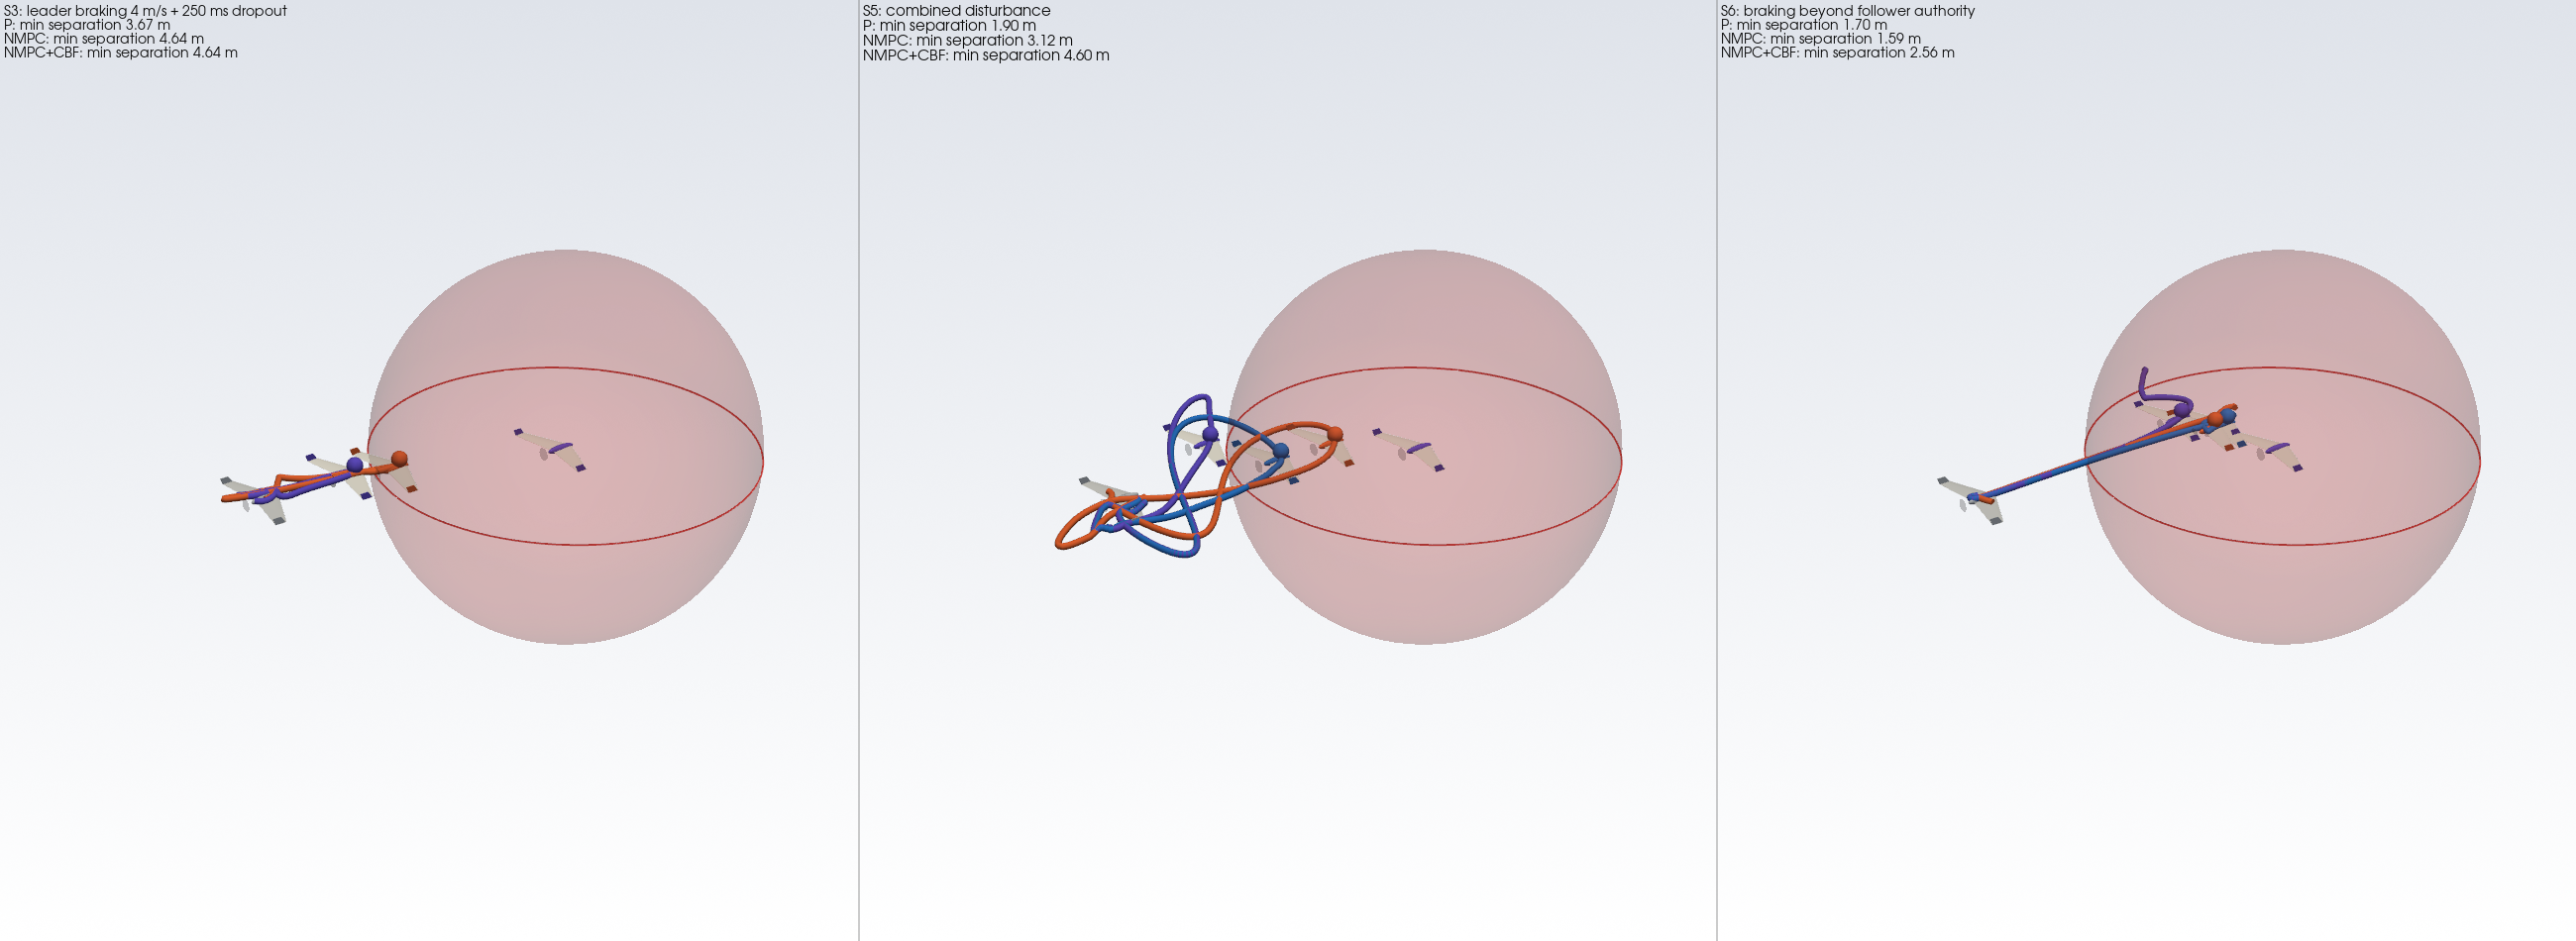
\includegraphics[width=\textwidth]{B1_safety_sphere}
\caption{Follower trajectories relative to the leader (real-scale meshes) around the $D_{\mathrm{safe}}=\SI{4.24}{m}$ sphere for the three controllers: braking with dropout (left), combined disturbance (centre), braking beyond follower authority (right). Spheres mark the closest approach.}\label{fig:B1}\end{figure}
\begin{table}[H]\centering\small
\caption{Control campaign, mean RMS lateral error (m) / worst-case minimum separation (m) / trials with $h<0$ (\%), 30 seeds each. $D_{\mathrm{safe}}=\SI{4.24}{m}$.}\label{tab:control}
\resizebox{\textwidth}{!}{\begin{tabular}{@{}lccc@{}}\toprule Scenario & PD & NMPC & NMPC+HOCBF \\ \midrule
S1 turbulence & 0.30 / 5.29 / 0 & 0.16 / 5.50 / 0 & 0.16 / 5.50 / 0 \\
S2 gust doublet 8.5 m/s & 0.48 / 5.29 / 0 & 0.46 / 5.50 / 0 & 0.54 / 5.50 / 0 \\
S3 leader braking + dropout & 0.31 / 2.12 / 100 & 0.17 / 3.30 / 37 & 0.17 / 3.30 / 37 \\
S4 degraded GNSS & 1.30 / 2.19 / 20 & 1.38 / 2.13 / 20 & 1.38 / 2.13 / 20 \\
S5 combined & 0.93 / 0.06 / 83 & 0.75 / 1.04 / 30 & 0.90 / 2.27 / 17 \\
S6 over-capability braking & 0.47 / 0.84 / 100 & 0.25 / 1.14 / 100 & 1.55 / 1.78 / 100
\\
\bottomrule\end{tabular}}\end{table}

Under turbulence the NMPC halves the PD baseline's lateral error (\nrmsEySOneN{} vs.\ \nrmsEySOneP{} m RMS; Table~\ref{tab:control}). The \SI{8.5}{m/s} differential gust doublet causes no violations for any controller (RMS \nrmsEySTwoN{}--\nrmsEySTwoC{} m). The safety filter's value is limited and conditional: in the braking-with-dropout scenario the PD baseline violates the safe set in \nviolSThreeP\,\% of trials, the NMPC in \nviolSThreeN\,\%, and adding the HOCBF changes nothing (\nviolSThreeC\,\%; active \nactSThreeC\,\% of the time) because the closure is longitudinal and bounded by deceleration authority; in the combined scenario the filter reduces violations from \nviolSFiveN\,\% to \nviolSFiveC\,\%; in the over-capability scenario every controller violates in \nviolSSixC\,\% of trials, and the filter increases lateral error to \nrmsEySSixC\,m without preventing the violation. Degraded GNSS leads to violations in \nviolSFourC\,\% of trials for all controllers since the filter acts on a biased measurement. Thus a barrier-function constraint is not a collision-avoidance guarantee once actuator saturation, model mismatch or measurement bias are present; we recorded no QP infeasibility events (\ncbfInfeas) because the filter's QP always had a bounded solution, not because the constraint was always satisfiable.

\subsubsection{Statistics of the control campaign}
Figure~\ref{fig:X11} gives distributions rather than means. The empirical CDF of the RMS lateral error in the combined scenario shows that the NMPC is better than the PD controller in almost every realisation, with a heavy upper tail caused by the degraded-GNSS component (a \SI{1.5}{m} bias cannot be controlled away because the controller does not observe it). The worst-case NMPC solve time per run was \SI{\nsolveMax}{ms} against a \SI{100}{ms} budget; the CBF-QP adds about \SI{0.3}{ms}. The mean peak lateral error ranks the scenarios in the order of difficulty S1 $<$ S3 $<$ S2 $<$ S5 $<$ S4 $\approx$ S6.
\begin{figure}[H]\centering\includegraphics[width=\textwidth]{X11_control_statistics}
\caption{(a) CDF of RMS lateral error (S5, 30 seeds); (b) CDF of the worst NMPC solve time per run (log axis); (c) mean peak lateral error by scenario and controller.}\label{fig:X11}\end{figure}

\subsubsection{Step response}
A \SI{1}{m} lateral slot step commanded over \SI{0.4}{s} without disturbances gives the loop characteristics in Fig.~\ref{fig:X12}b: overshoot \nstepPOver\,\% for the PD law, \nstepNOver\,\% for the NMPC and \nstepCOver\,\% with the filter; $2\,\%$ settling time \nstepPSettle, \nstepNSettle{} and \nstepCSettle\,s; 10--90\,\% rise time \nstepPRise, \nstepNRise{} and \nstepCRise\,s. The bank angle never exceeds the \SI{35}{\degree} limit. The filter is inactive in this test because the barrier is far from violated.

\subsubsection{Margin ablation of the safety filter}
The HOCBF margin $\Delta D$ (added to $D_{\mathrm{safe}}$) trades safety for wake benefit because a more conservative filter deflects the follower from the slot more often. Figure~\ref{fig:X12}a--c shows the violation rate, tracking error and mean drag-coefficient saving for $\Delta D\in\{0,0.5,1,2\}$\,m over 16 seeds per scenario. In the braking scenario (S3) violations are \ncbfThreeVMzero\,\%, \ncbfThreeVMhalf\,\%, \ncbfThreeVMone\,\% and \ncbfThreeVMtwo\,\% for the four margins, with mean lateral error \ncbfThreeEMzero, \ncbfThreeEMhalf, \ncbfThreeEMone and \ncbfThreeEMtwo\,m; in the combined scenario (S5) the violation rates are \ncbfFiveVMzero, \ncbfFiveVMhalf, \ncbfFiveVMone and \ncbfFiveVMtwo\,\%; in the over-capability scenario (S6) \ncbfSixVMzero, \ncbfSixVMhalf, \ncbfSixVMone and \ncbfSixVMtwo\,\%. The saving index (mean drag-coefficient reduction in units of $10^{-4}$) is \ncbfFiveSMzero, \ncbfFiveSMhalf, \ncbfFiveSMone and \ncbfFiveSMtwo for S5. The first-order message is that margin cannot substitute for authority: when the leader decelerates faster than the follower can, no margin avoids the violation, and a larger margin only reduces the wake benefit.
\begin{figure}[H]\centering\includegraphics[width=\textwidth]{X12_cbf_margin_ablation}
\caption{HOCBF margin ablation (16 seeds per point): (a) fraction of runs with $h<0$; (b) RMS lateral error; (c) mean drag-coefficient reduction from the realised slot error (VLM sheet). Right panel of the next figure: step-response metrics.}\label{fig:X12}\end{figure}
\begin{figure}[H]\centering\includegraphics[width=0.55\textwidth]{X12b_step_response}
\caption{Overshoot and 2\,\% settling time for a \SI{1}{m} lateral step (3 seeds, no disturbances).}\label{fig:X12b}\end{figure}


\subsection{Reconfiguration cost}\label{sec:reconf}
Splitting into zones (\SI{369.6}{m} lateral displacement) was simulated for five peak lateral speeds. The energy above isolated cruise over the manoeuvre window is \novFast\,Wh at \ntFast\,s and \novSlow\,Wh at \ntSlow\,s (\novMid\,Wh at \ntMid\,s), per follower, including the lost wake benefit. The preliminary version charged \SI{\nmanuReconf}{Wh} (three aircraft $\times$\,\SI{45}{s} at full cruise power) \emph{on top of} the time already counted. \begin{figure}[H]\centering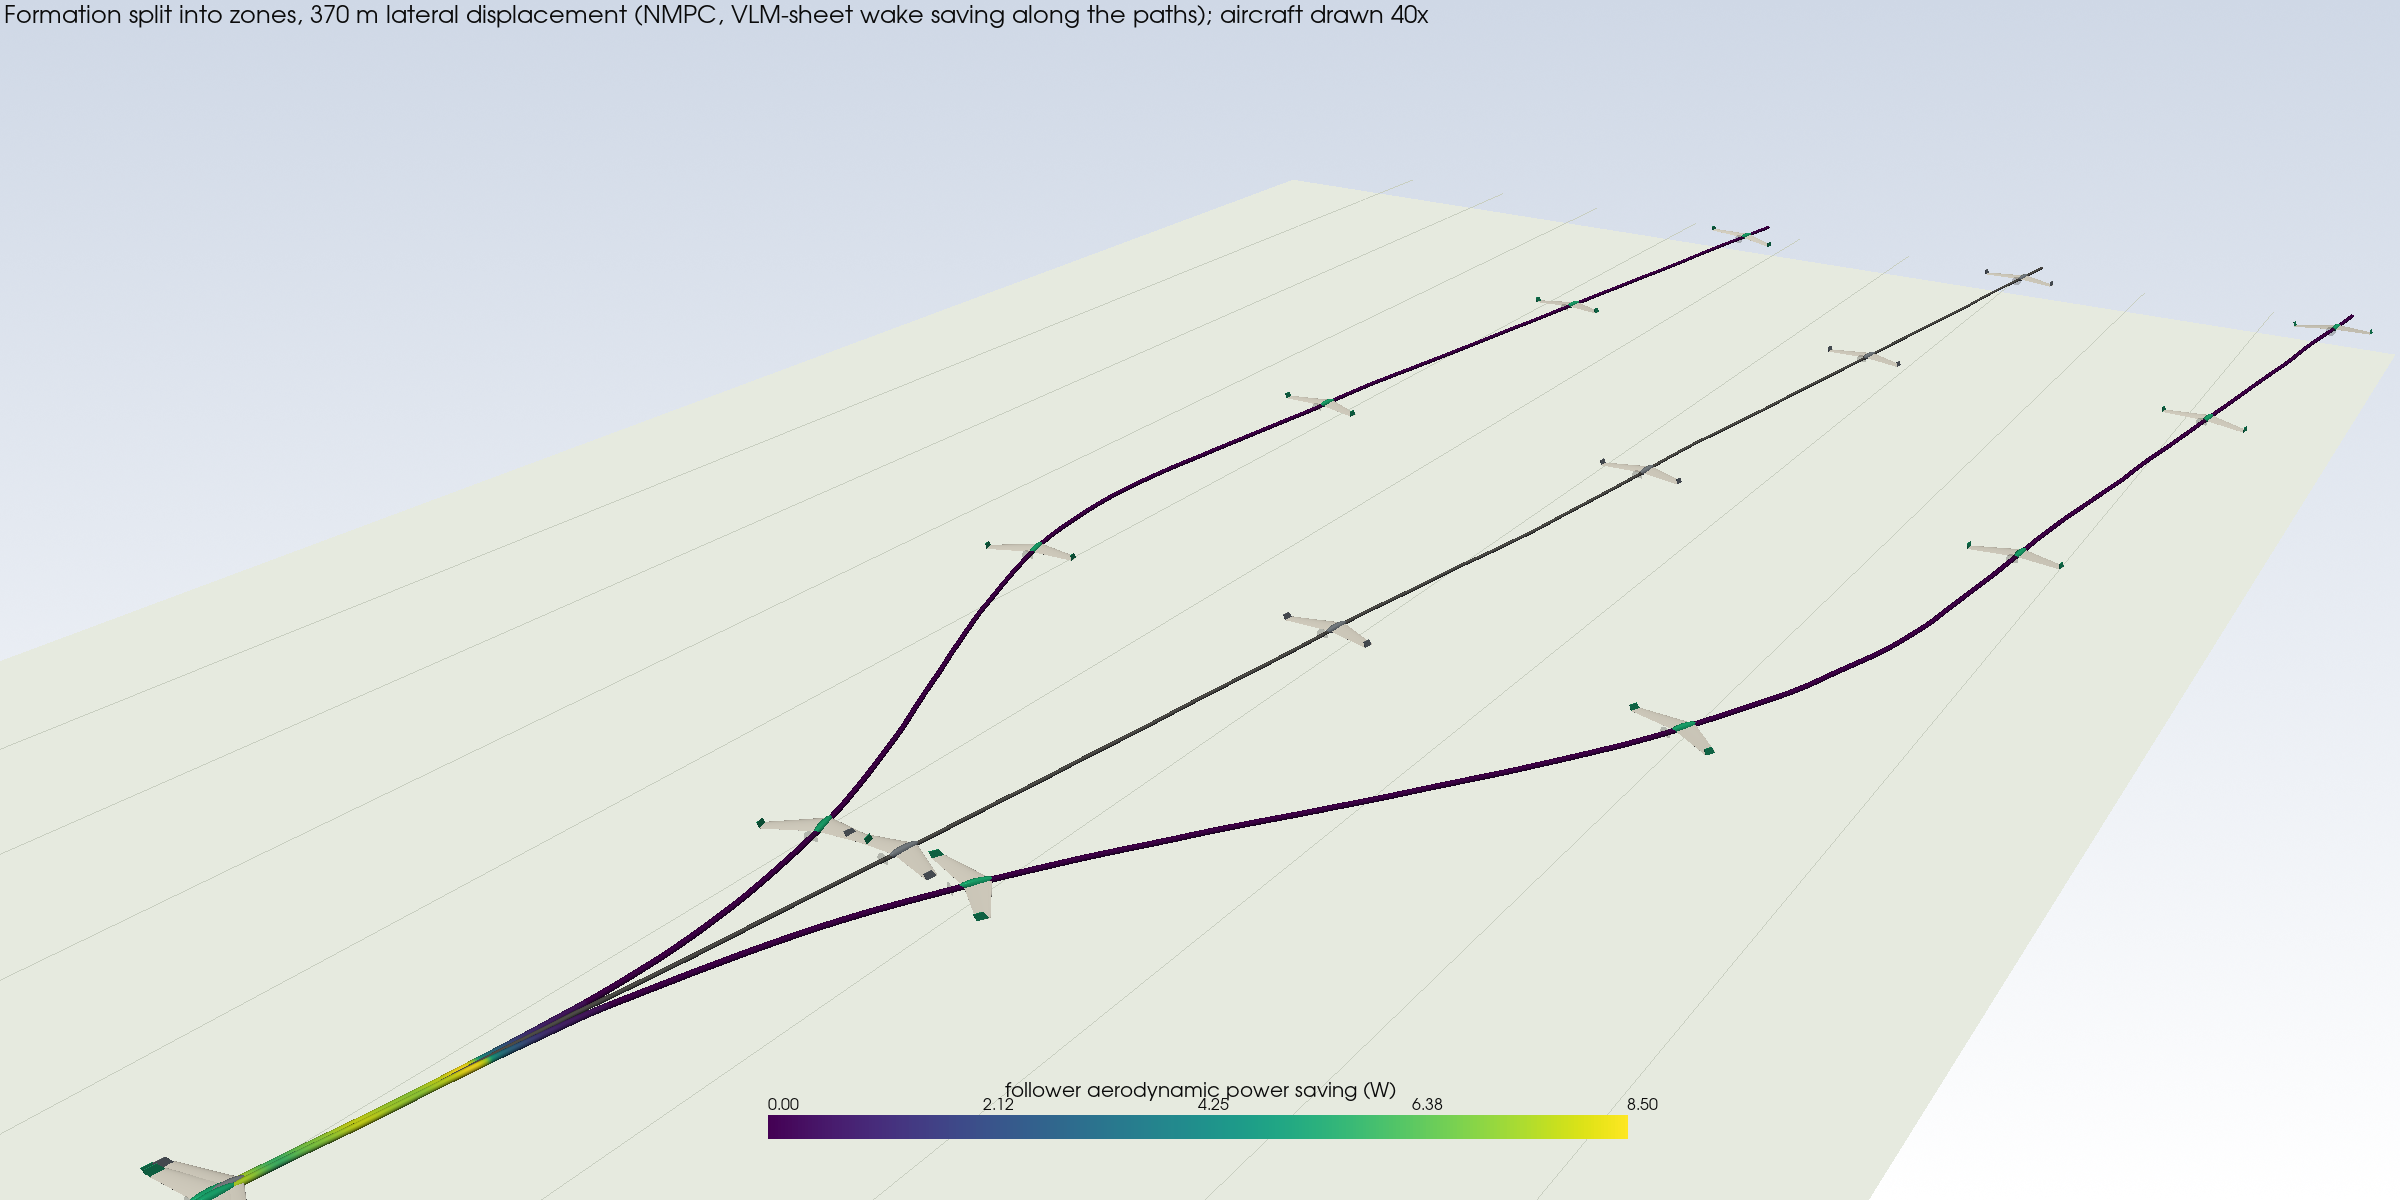
\includegraphics[width=\textwidth]{B2_split_manoeuvre}
\caption{Split of the formation into zones (\SI{370}{m} lateral displacement, NMPC). Follower paths are coloured by the instantaneous aerodynamic power saving (VLM planar sheet): the saving vanishes within seconds of leaving the slot. Aircraft are drawn 40$\times$.}\label{fig:B2}\end{figure}
The real penalties are different: the manoeuvre occupies a large share of a \SI{2.5}{km} transit (\SI{>60}{s} of \SI{139}{s}), so the wake is harvested only briefly, and the early-finishing aircraft must wait for the slowest before re-forming (waiting energy \nwaitSFour\,Wh for S4).

\subsubsection{Reconfiguration energy law}
The simulated windows give a smooth law (Fig.~\ref{fig:X7}): for a fixed lateral displacement the energy above isolated cruise falls as the window lengthens (lower lateral speed, smaller heading change, smaller airspeed excess) while the wake benefit lost grows with the time spent outside the slot. For the \SI{369.6}{m} split the net overhead per follower is \novFast\,Wh at \ntFast\,s, \novMid\,Wh at \ntMid\,s and \novSlow\,Wh at \ntSlow\,s; the \SI{60}{m} join-up and break-up cost under \SI{0.1}{Wh} each. The maximum bank angle in these manoeuvres is $8$--$10^\circ$ for the long splits and $13$--$21^\circ$ for the short joins (peak lateral speed \SIrange{8}{12}{m/s}), within the \SI{35}{\degree} limit. Merge and split are close to mirror images of each other, differing mainly in where the wake benefit is regained or lost.
\begin{figure}[H]\centering\includegraphics[width=\textwidth]{X7_reconfiguration_law}
\caption{Follower energy above isolated cruise versus (a) window duration and (b) peak lateral speed; (c) maximum bank angle. Splits (circles) and merges (squares) for $Y=\SI{60}{m}$ and \SI{369.6}{m}.}\label{fig:X7}\end{figure}


\subsection{Mission energy per accepted hectare}\label{sec:mission}
\begin{table}[H]\centering\small
\caption{Mission outcomes, VLM planar-sheet model, mean $\pm$ SD over \nnTrials{} paired trials. Accepted area is geometric (criteria 1--2 only).}\label{tab:strat}
\resizebox{\textwidth}{!}{\begin{tabular}{@{}lccccc@{}}\toprule Strategy & $E_{\mathrm{fleet}}$ (Wh) & max per-UAV (Wh) & time (min) & acc.\ (ha) & $\Earea$ (Wh/ha)\\\midrule
S1 Independent & 112.9 $\pm$ 2.1 & 38.0 & 15.2 & 100 & 1.129 $\pm$ 0.021  \\
S2 Rigid V & 224.1 $\pm$ 4.2 & 74.7 & 31.2 & 100 & 2.241 $\pm$ 0.042  \\
S3 Adaptive geometric V & 114.4 $\pm$ 2.0 & 38.6 & 15.2 & 100 & 1.144 $\pm$ 0.020  \\
S4 Wake-aware adaptive V & 109.1 $\pm$ 2.0 & 37.4 & 14.7 & 100 & 1.091 $\pm$ 0.020  \\
D1 Independent, 14-strip route & 104.9 $\pm$ 1.9 & 36.8 & 14.7 & 100 & 1.049 $\pm$ 0.019 
\\
\bottomrule\end{tabular}}\end{table}
\begin{table}[H]\centering\small
\caption{Change in $\Earea$ relative to the reference (\%): mean (5th, 95th percentile of trials) for five aerodynamic models. Negative = saving.}\label{tab:paired}
\resizebox{\textwidth}{!}{\begin{tabular}{@{}lcccc@{}}\toprule Comparison & VLM sheet & VLM free wake & Strip, corrected & As published\\\midrule
S4 vs S1 (full framework) & -3.4 (-3.4, -3.3) & -3.3 (-3.4, -3.3) & -3.2 (-3.3, -3.2) & -3.2 (-3.3, -3.2) & -2.4 (-2.6, -2.1) \\
S3 vs S1 (formation only) & +1.4 (+1.3, +1.5) & +1.4 (+1.3, +1.5) & +1.5 (+1.4, +1.6) & +1.5 (+1.4, +1.6) & +2.4 (+2.2, +2.7) \\
S2 vs S1 (rigid V) & +98.5 (+98.4, +98.7) & +98.9 (+98.8, +99.2) & +100.2 (+100.1, +100.4) & +100.4 (+100.2, +100.7) & +108.7 (+106.4, +112.0) \\
S3 vs S2 (adaptive vs rigid) & -48.9 (-49.0, -48.9) & -49.0 (-49.1, -49.0) & -49.3 (-49.4, -49.2) & -49.3 (-49.4, -49.3) & -50.9 (-51.6, -50.5) \\
S4 vs D1 (formation, 14-strip route) & +4.0 (+3.9, +4.1) & +4.1 (+4.0, +4.1) & +4.2 (+4.1, +4.2) & +4.2 (+4.1, +4.2) & +5.1 (+4.9, +5.4) \\
D1 vs S1 (route/overlap only) & -7.1 (-7.1, -7.1) & -7.1 (-7.1, -7.1) & -7.1 (-7.1, -7.1) & -7.1 (-7.1, -7.1) & -7.1 (-7.1, -7.1)
\\
\bottomrule\end{tabular}}\end{table}
\begin{figure}[H]\centering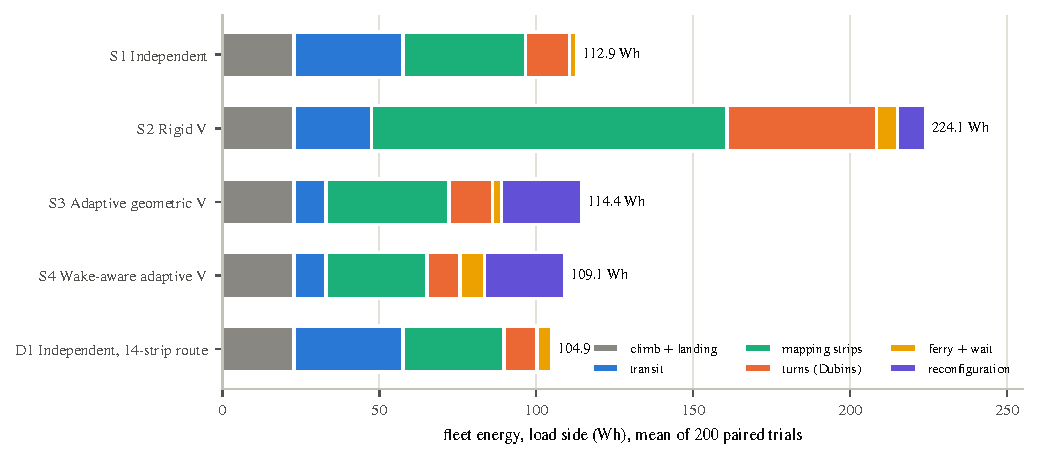
\includegraphics[width=0.95\textwidth]{fig09_energy_breakdown}
\caption{Phase breakdown of fleet energy (VLM sheet, mean of \nnTrials{} trials).}\label{fig:break}\end{figure}
\begin{figure}[H]\centering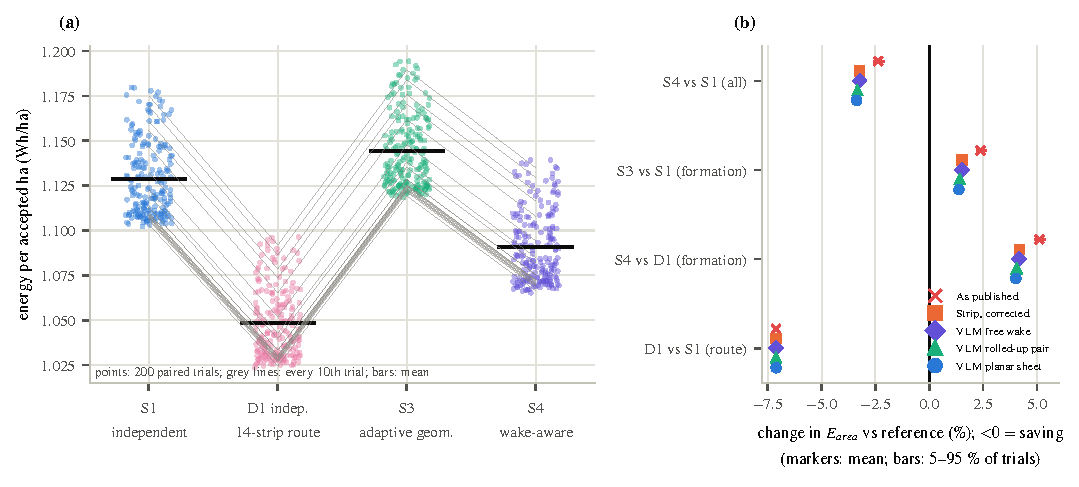
\includegraphics[width=\textwidth]{fig10_energy_efficiency}
\caption{(a) Energy per accepted hectare, raw paired trials. (b) Change vs.\ reference for five aerodynamic models (markers) with 5--95\,\% trial range (bars).}\label{fig:eff}\end{figure}
\begin{figure}[H]\centering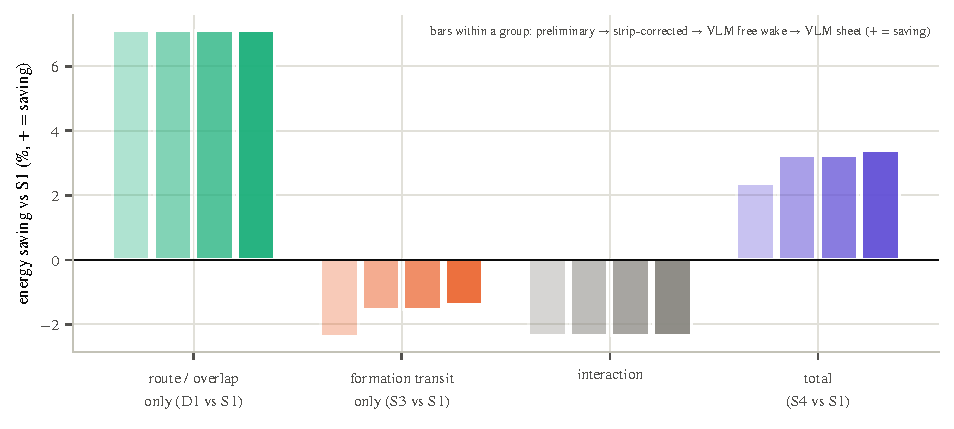
\includegraphics[width=0.85\textwidth]{fig15_decomposition}
\caption{Factorial decomposition of the S4-vs-S1 difference into formation-transit, route/overlap and interaction components (positive = saving).}\label{fig:dec}\end{figure}
\begin{figure}[H]\centering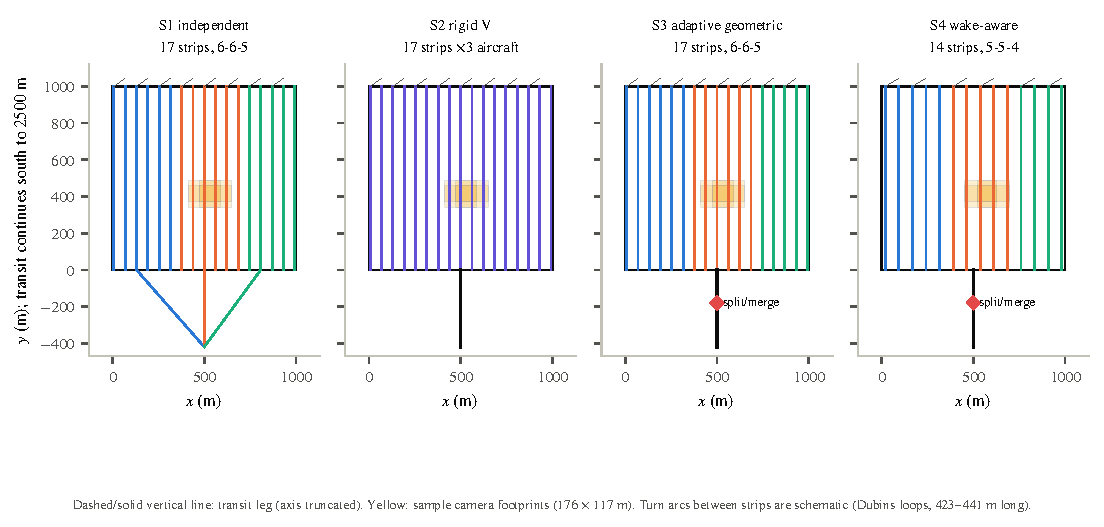
\includegraphics[width=\textwidth]{fig06_mission_comparison}
\caption{The \SI{100}{ha} polygon under the four strategies (turn loops schematic).}\label{fig:missions}\end{figure}
\begin{figure}[H]\centering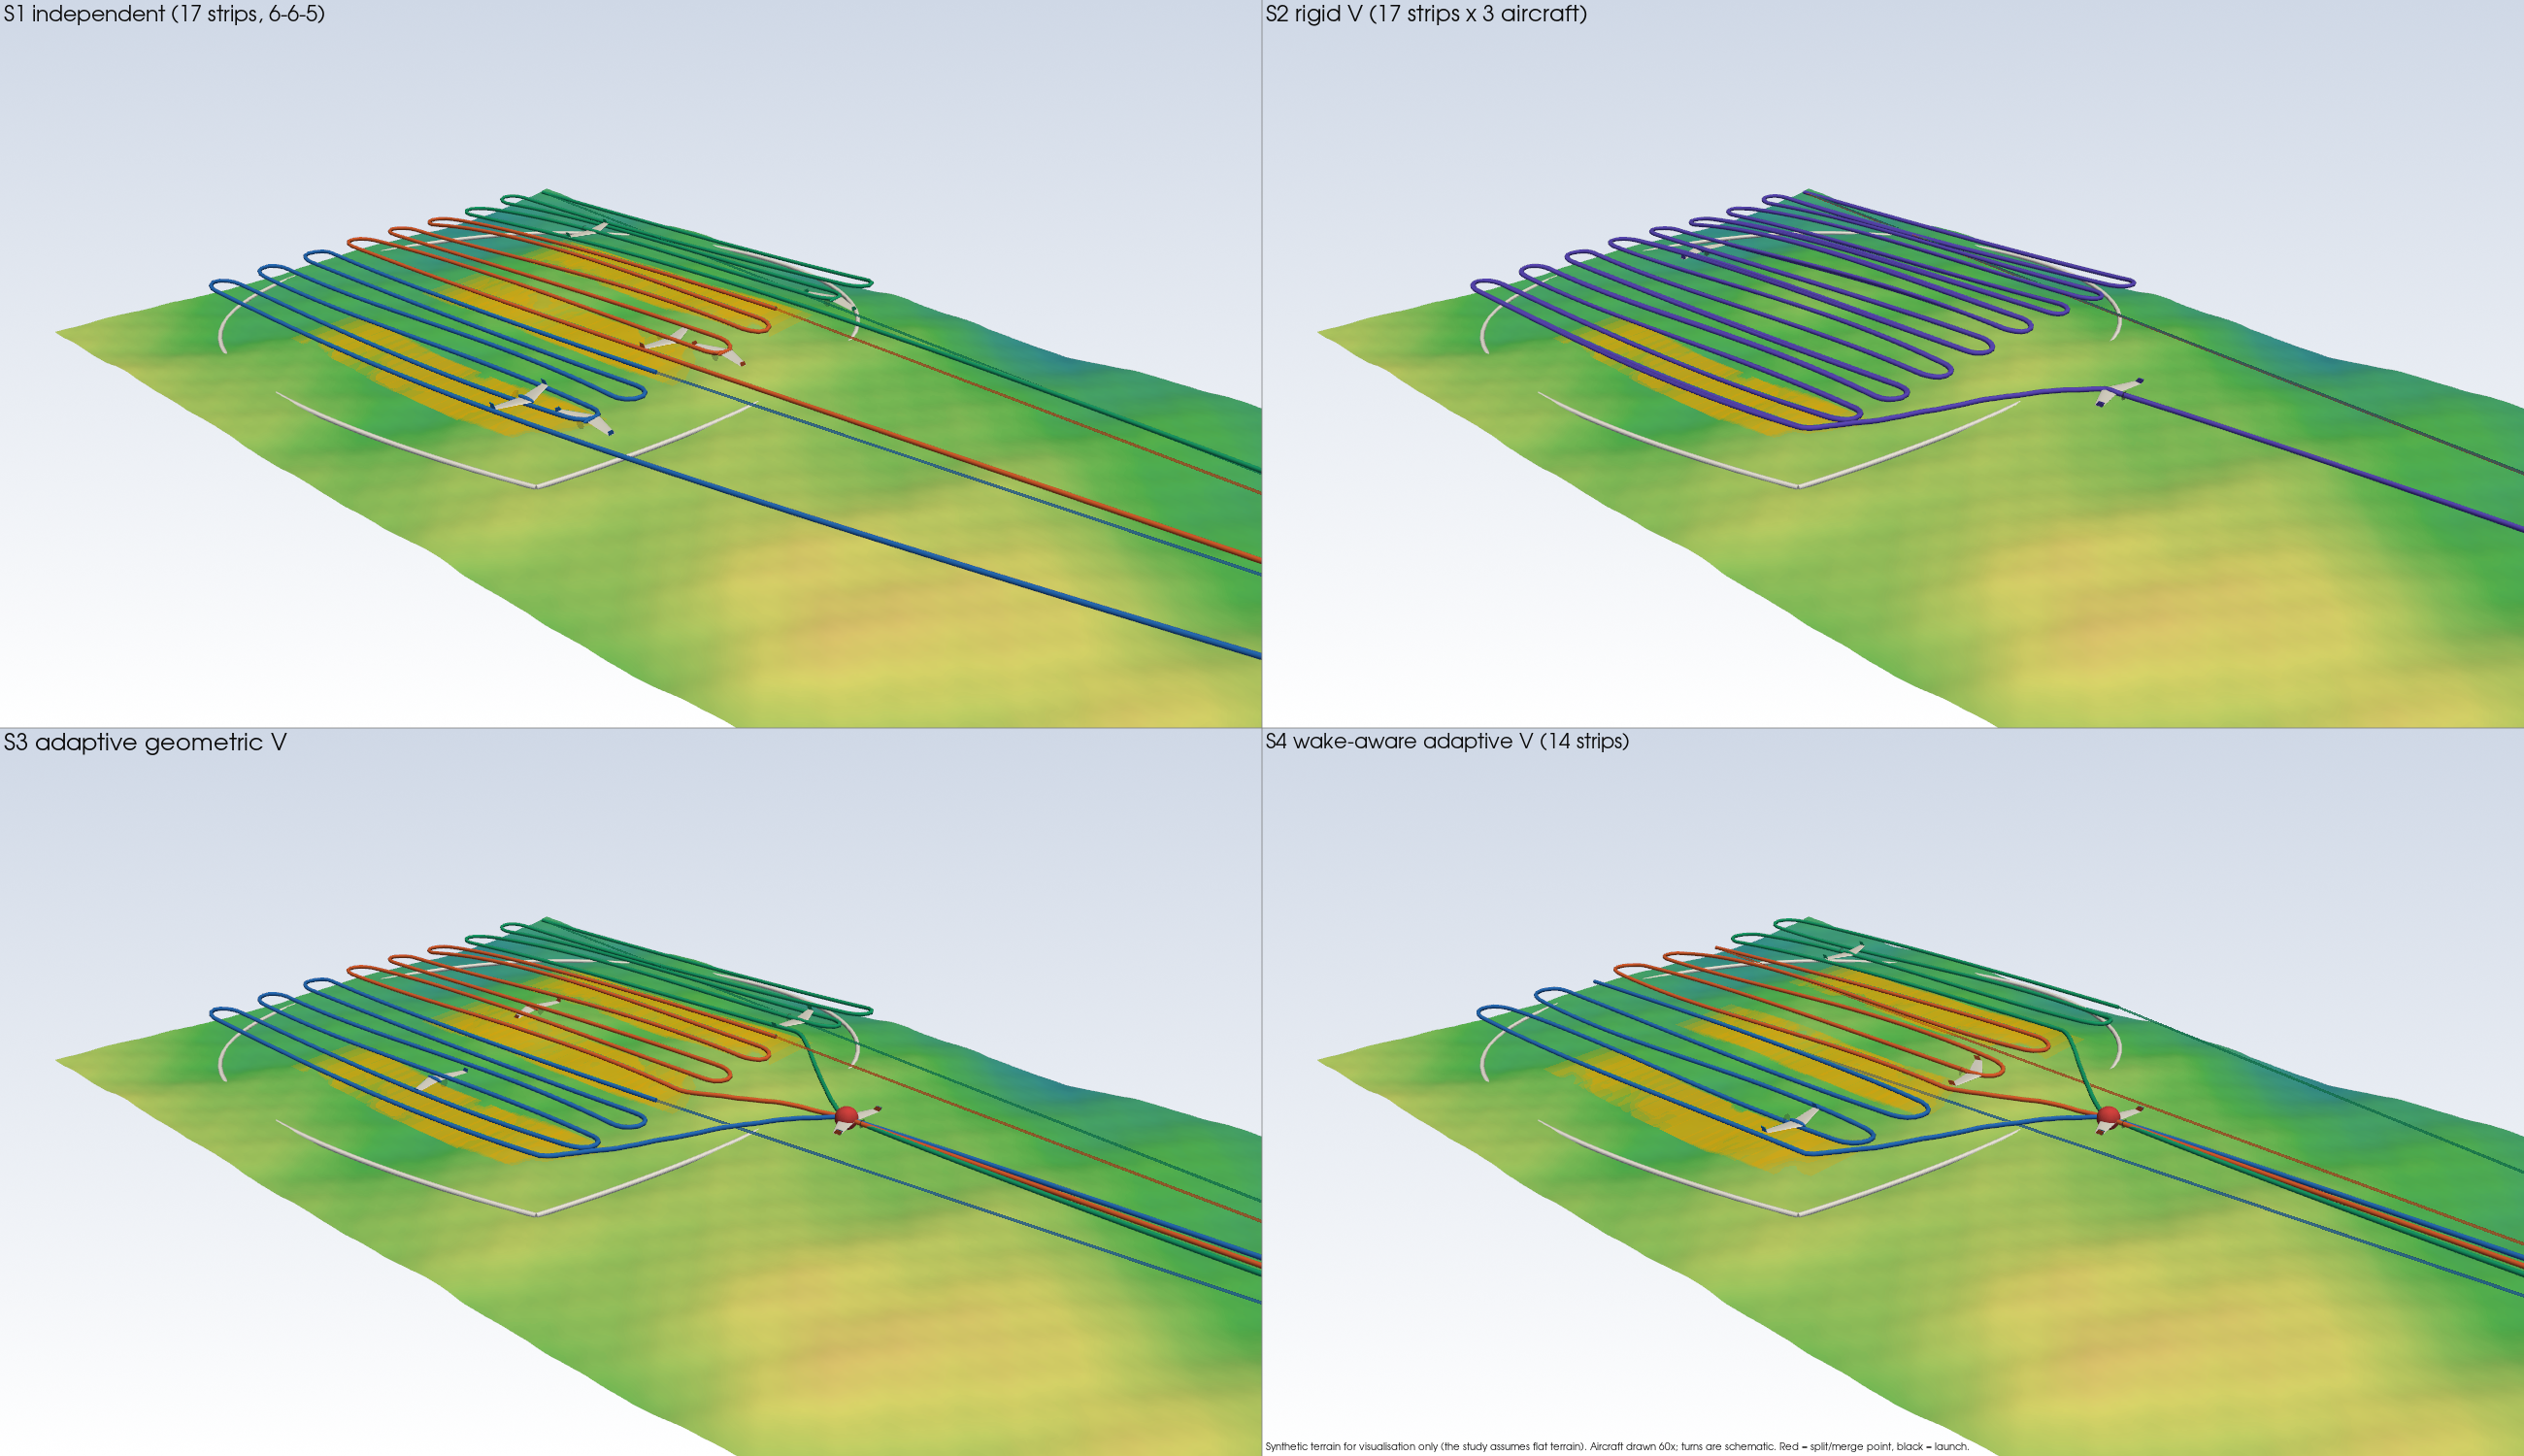
\includegraphics[width=\textwidth]{D1_mission_overview}
\caption{Three-dimensional view of the four strategies over synthetic terrain (terrain for visualisation only; the study assumes flat ground). Tubes: flight paths at \SI{120}{m} AGL by aircraft; yellow: camera footprints; red sphere: split/merge point. Aircraft drawn 60$\times$.}\label{fig:D1}\end{figure}

Table~\ref{tab:strat} and Figs.~\ref{fig:break}--\ref{fig:eff} give the results. Every strategy is feasible within the \SI{80}{\percent} usable-battery limit (max per-UAV load \nmisEmaxSOne\,Wh for S1 of about \SI{178}{Wh} usable). Climb and landing alone cost \nclimbLand\,Wh of S1's fleet energy and the Dubins turns \nturnsOne\,Wh, which dilute any percentage saving relative to a model that ignores them. The rigid V (S2) uses \nrelCSheet\,\% more energy per accepted hectare than S1, because it flies three times the track for identical coverage (S3 vs.\ S2: \nrelDSheet\,\%). The full framework (S4) changes $\Earea$ by \nrelASheet\,\% with the VLM model (\nrelAPub\,\% with the published equations), well below the \SI{5}{\percent} threshold set in the preliminary version.

The decomposition (Fig.~\ref{fig:dec}) shows \emph{where} it comes from. Moving to the 14-strip route without formation (D1) saves \nrelFSheet\,\%. Formation transit on the unchanged 17-strip route (S3) \emph{costs} \nrelBSheet\,\% (\ndWhB\,Wh per mission), and on the 14-strip route (S4 vs.\ D1) \nrelESheet\,\%. In energy terms: formation only \ndecFormSheet\,Wh, route/overlap only \ndecRouteSheet\,Wh, interaction \ndecInterSheet\,Wh, total \ndecTotSheet\,Wh of S1's \nmisESOne\,Wh. The interaction is negative because the 5-5-4 split is less balanced (waiting) and the formation overhead is paid for four events. Hence, within this model, the 58\,\% side-overlap assumption, available to independent aircraft with RTK, not the wake, produces the gain: the framework's central claim of an aerodynamic benefit is not supported at \SI{2.5}{km}.

\subsubsection{Mission timelines and the structure of the energy budget}
Figure~\ref{fig:X9} shows the power drawn by each aircraft over time for one wind realisation. The aerodynamic benefit is invisible at this scale: the followers' transit power differs from the leader's by $\approx$\SI{8}{W} on \SI{143}{W}, and the dominant structures are the mapping legs and the turns (the Dubins loops of the 17-strip plan are visible as the orange blocks between mapping legs). The strategies with formation differ from S1 by the reconfiguration blocks (violet) at the start, the split, the merge and the break-up, and by the waiting blocks (magenta) of the aircraft that finish early. This is the structural reason that the formation overheads, small in isolation, add up to more than the aerodynamic saving at \SI{2.5}{km}.
\begin{figure}[H]\centering\includegraphics[width=\textwidth]{X9_power_timeline}
\caption{Load power versus time for the three aircraft (rows) under S1, S3 and S4 (columns) for one environment realisation (wind \SI{3.5}{m/s}); colours are mission phases.}\label{fig:X9}\end{figure}

\subsubsection{Leader rotation and battery balance}
Because only the followers profit from the wake, a fixed leader would carry the full cost of the formation phases. Rotating the role cyclically makes the formation-phase energy identical for the three aircraft; without rotation the leader would spend about \SI{4}{Wh} more than a follower over the S3 transit (Fig.~\ref{fig:X10}b), which is \SI{10}{\percent} of the aircraft's mission energy. The maximum per-aircraft energy of S3 and S4 is \nmisEmaxSThree\ and \nmisEmaxSFour\,Wh, against \nmisEmaxSOne\,Wh for S1; the usable battery (\SI{177.6}{Wh}) is never approached by any strategy except the rigid V, whose per-aircraft energy is \nmisEmaxSTwo\,Wh.
\begin{figure}[H]\centering\includegraphics[width=\textwidth]{X10_leader_rotation_energy}
\caption{(a) Per-aircraft energy (maximum, filled circle, and minimum, open circle, over the three aircraft; mean $\pm$ SD over trials) for four strategies, against the usable battery energy; (b) leader-minus-follower energy gap over the S3 formation transit that cyclic rotation eliminates.}\label{fig:X10}\end{figure}

\subsubsection{Monte-Carlo diagnostics}
The paired difference S3$-$S1 has a mean of \nmcDiffMean\,Wh and a trial-to-trial SD of only \nmcDiffSD\,Wh (Fig.~\ref{fig:X8}a): the running mean has converged to within a few hundredths of a watt-hour after $\approx$40 trials, and the bootstrap interval is narrower than the line width beyond 80. By contrast, the energy of a single strategy varies by \nmcRange\,Wh over the wind range (SD \nmcSDOne\,Wh); a linear regression on wind speed alone explains $R^2=\nmcRTwo$ of that variance with a slope of \nmcSlope\,Wh per m/s (Fig.~\ref{fig:X8}b), i.e.\ the strip headwind/tailwind asymmetry and the longer ground-speed-limited legs. The strategy \emph{difference} depends only weakly on the wind: a harmonic regression on wind direction explains $R^2=\nmcDirRTwo$ of its variance (Fig.~\ref{fig:X8}c). Tight paired intervals here therefore document simulation determinism, not field repeatability.
\begin{figure}[H]\centering\includegraphics[width=\textwidth]{X8_monte_carlo_diagnostics}
\caption{(a) Running mean of the S3$-$S1 difference with bootstrap 95\,\% interval versus number of trials; (b) S1 energy versus wind speed (colour: wind direction); (c) S3$-$S1 versus wind direction (polar).}\label{fig:X8}\end{figure}


\subsection{Break-even and sensitivity}\label{sec:sens}
\begin{figure}[H]\centering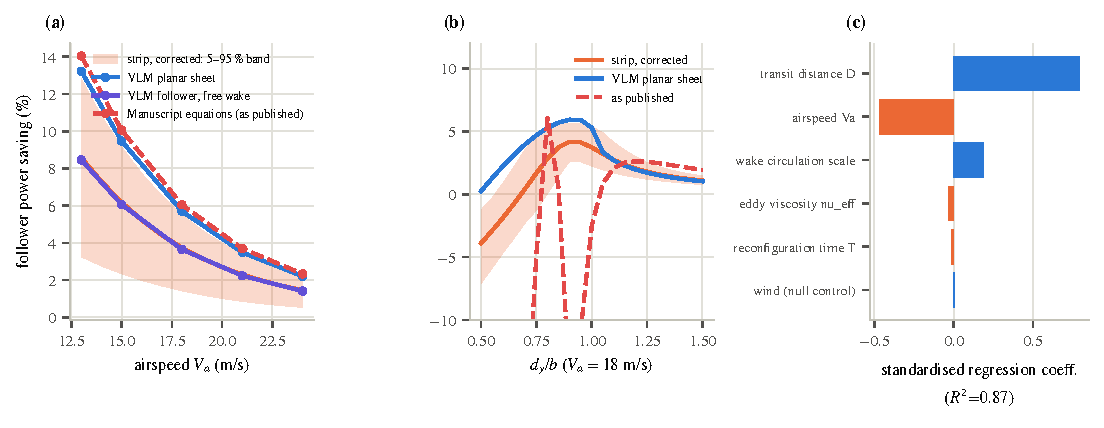
\includegraphics[width=\textwidth]{fig11_sensitivity}
\caption{(a) Saving vs.\ airspeed with parametric uncertainty band; (b) saving vs.\ offset; (c) standardised regression coefficients of the net formation effect ($R^2=\nsrcRtwo$). ``Wind'' is a negative-control input with no path to the output.}\label{fig:sens}\end{figure}
\begin{figure}[H]\centering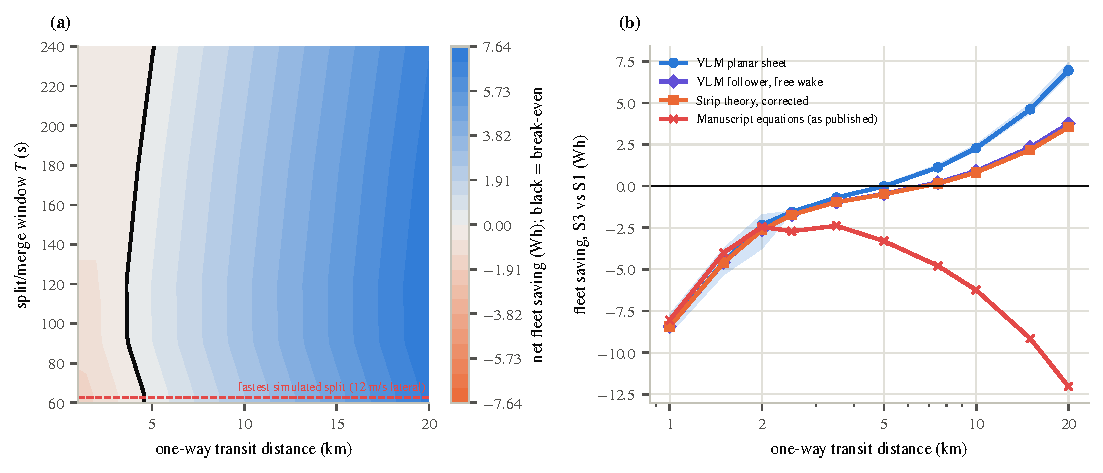
\includegraphics[width=\textwidth]{fig12_breakeven}
\caption{(a) Net fleet saving of formation transit over a split/merge window $T$ and one-way distance (VLM sheet; window times below \SI{62.7}{s} would need $>12$\,m/s lateral speed and are not simulated). (b) Mission-simulator saving of S3 vs.\ S1 vs.\ distance; band: 5--95\,\% of trials. For $D\lesssim 2$\,km the fastest manoeuvre exceeds the available transit and the result is a lower bound.}\label{fig:be}\end{figure}
Formation transit on the 17-strip route breaks even at about \nbeSevSheet\,km one-way with the VLM sheet, \nbeSevFree\,km with the free wake and \nbeSevStrip\,km with corrected strip theory; with the published equations it never does, because realised station-keeping errors of order \SI{0.1}{m} fall off the published knife-edge. On the 14-strip route the break-even is \nbeFourteenSheet\,km (sheet) to \nbeFourteenFree\,km (free wake) because of the larger waiting penalty. The global sensitivity (Fig.~\ref{fig:sens}c, $R^2=\nsrcRtwo$) ranks transit distance ($\nsrcD$) above airspeed ($\nsrcV$), wake-circulation scale ($\nsrcG$), and shows negligible dependence on reconfiguration window ($\nsrcT$) within the simulated range and on viscosity ($\nsrcNu$); the null-control factor is \nsrcW. Flying the formation slower raises the \emph{percentage} saving (VLM: \nsheetVEighteen\,\% at \SI{18}{m/s} to \nsheetVThirteen\,\% at \SI{13}{m/s}, each against the isolated aircraft at the same speed) but lengthens the transit and therefore the time over which the hotel load is paid; the mission simulations here use a single \SI{18}{m/s} cruise.

\subsubsection{Wake effectiveness versus distance}
Because the wake model is the dominant epistemic uncertainty, Fig.~\ref{fig:X2} maps the net fleet saving of formation transit over the wake-effectiveness factor $\kappa$ (the tabulated drag reduction is multiplied by $\kappa$; $\kappa=1$ is the planar sheet, $\kappa\approx0.7$ the free wake, $\kappa\approx0.9$ the strip model) and the one-way transit distance, with every other element of the mission simulator unchanged. The zero contour is nearly vertical in $\kappa$ at short range and bends towards short distances as $\kappa$ grows: at \SI{2.5}{km} the saving is \nkmAtTwoFive\,Wh for $\kappa=1$ and \nkmAtTwoFiveLow\,Wh for $\kappa=0.3$ (the difference is \SI{0.4}{Wh}: the transit wake benefit is almost irrelevant at that distance), while at \SI{20}{km} it ranges from small to \nkmAtTwoZerok\,Wh ($\kappa=1$). The break-even distance on the 17-strip route is \nkmBeOneSevenOne\,km at $\kappa=1$, \nkmBeOneSevenFree\,km at $\kappa=0.7$, \nkmBeOneSevenLow\,km at $\kappa=0.3$ and \nkmBeOneSevenHigh\,km at $\kappa=1.5$; on the 14-strip route (right panel) it is \nkmBeOneFourOne\,km at $\kappa=1$, \nkmBeOneFourFree\,km at $\kappa=0.7$, exceeds \SI{20}{km} (not reached within the simulated range) at $\kappa=0.3$, and is \nkmBeOneFourHigh\,km at $\kappa=1.5$. Even doubling the wake effectiveness over the best model leaves the break-even beyond \SI{4}{km}.
\begin{figure}[H]\centering\includegraphics[width=\textwidth]{X2_kappa_distance_map}
\caption{Net fleet saving of formation transit (positive = saving) over wake effectiveness $\kappa$ and one-way transit distance for (a) the 17-strip route (S3 vs S1) and (b) the 14-strip route (S4 vs D1). Dotted lines: values of $\kappa$ corresponding to the three wake models.}\label{fig:X2}\end{figure}

\subsubsection{One-at-a-time and variance-based sensitivity}
The tornado diagram (Fig.~\ref{fig:X3}a) varies one factor at a time around the baseline of the S3-versus-S1 fleet saving (\ntorBase\,Wh at \SI{2.5}{km}): wake effectiveness $\kappa\in[0.6,1.2]$ changes it by \ntorKappaLo{} and \ntorKappaHi\,Wh, the reconfiguration overhead ($0.6\times$--$1.6\times$) by \ntorReconfLo{} and \ntorReconfHi\,Wh, the station-keeping error ($0.5\times$--$3\times$) by \ntorErrLo{} and \ntorErrHi\,Wh, the wind-speed range centre (1--\SI{6}{m/s}) by \ntorWindLo{} and \ntorWindHi\,Wh, and the transit distance (1.5--\SI{10}{km}) by \ntorDistLo{} and \ntorDistHi\,Wh. Variance-based Sobol indices over the same ranges (pick--freeze estimator with $N=250$; Fig.~\ref{fig:X3}b) give first-order indices of \nsobDistS{} for distance, \nsobKappaS{} for $\kappa$, \nsobReconfS{} for reconfiguration, \nsobErrS{} for station keeping and \nsobWindS{} for wind (sum \nsobSumS); total-order indices are \nsobDistT, \nsobKappaT, \nsobReconfT, \nsobErrT{} and \nsobWindT. Transit distance dominates, followed by wake effectiveness; the interaction between them (their product is the integrated benefit) is visible as a gap between $S_i$ and $S_{Ti}$.
\begin{figure}[H]\centering\includegraphics[width=\textwidth]{X3_tornado_sobol}
\caption{(a) Tornado diagram of the S3-vs-S1 fleet saving (orange: low setting, blue: high setting); (b) Sobol first-order and total indices.}\label{fig:X3}\end{figure}


\subsection{Coverage geometry}\label{sec:geom}
\begin{figure}[H]\centering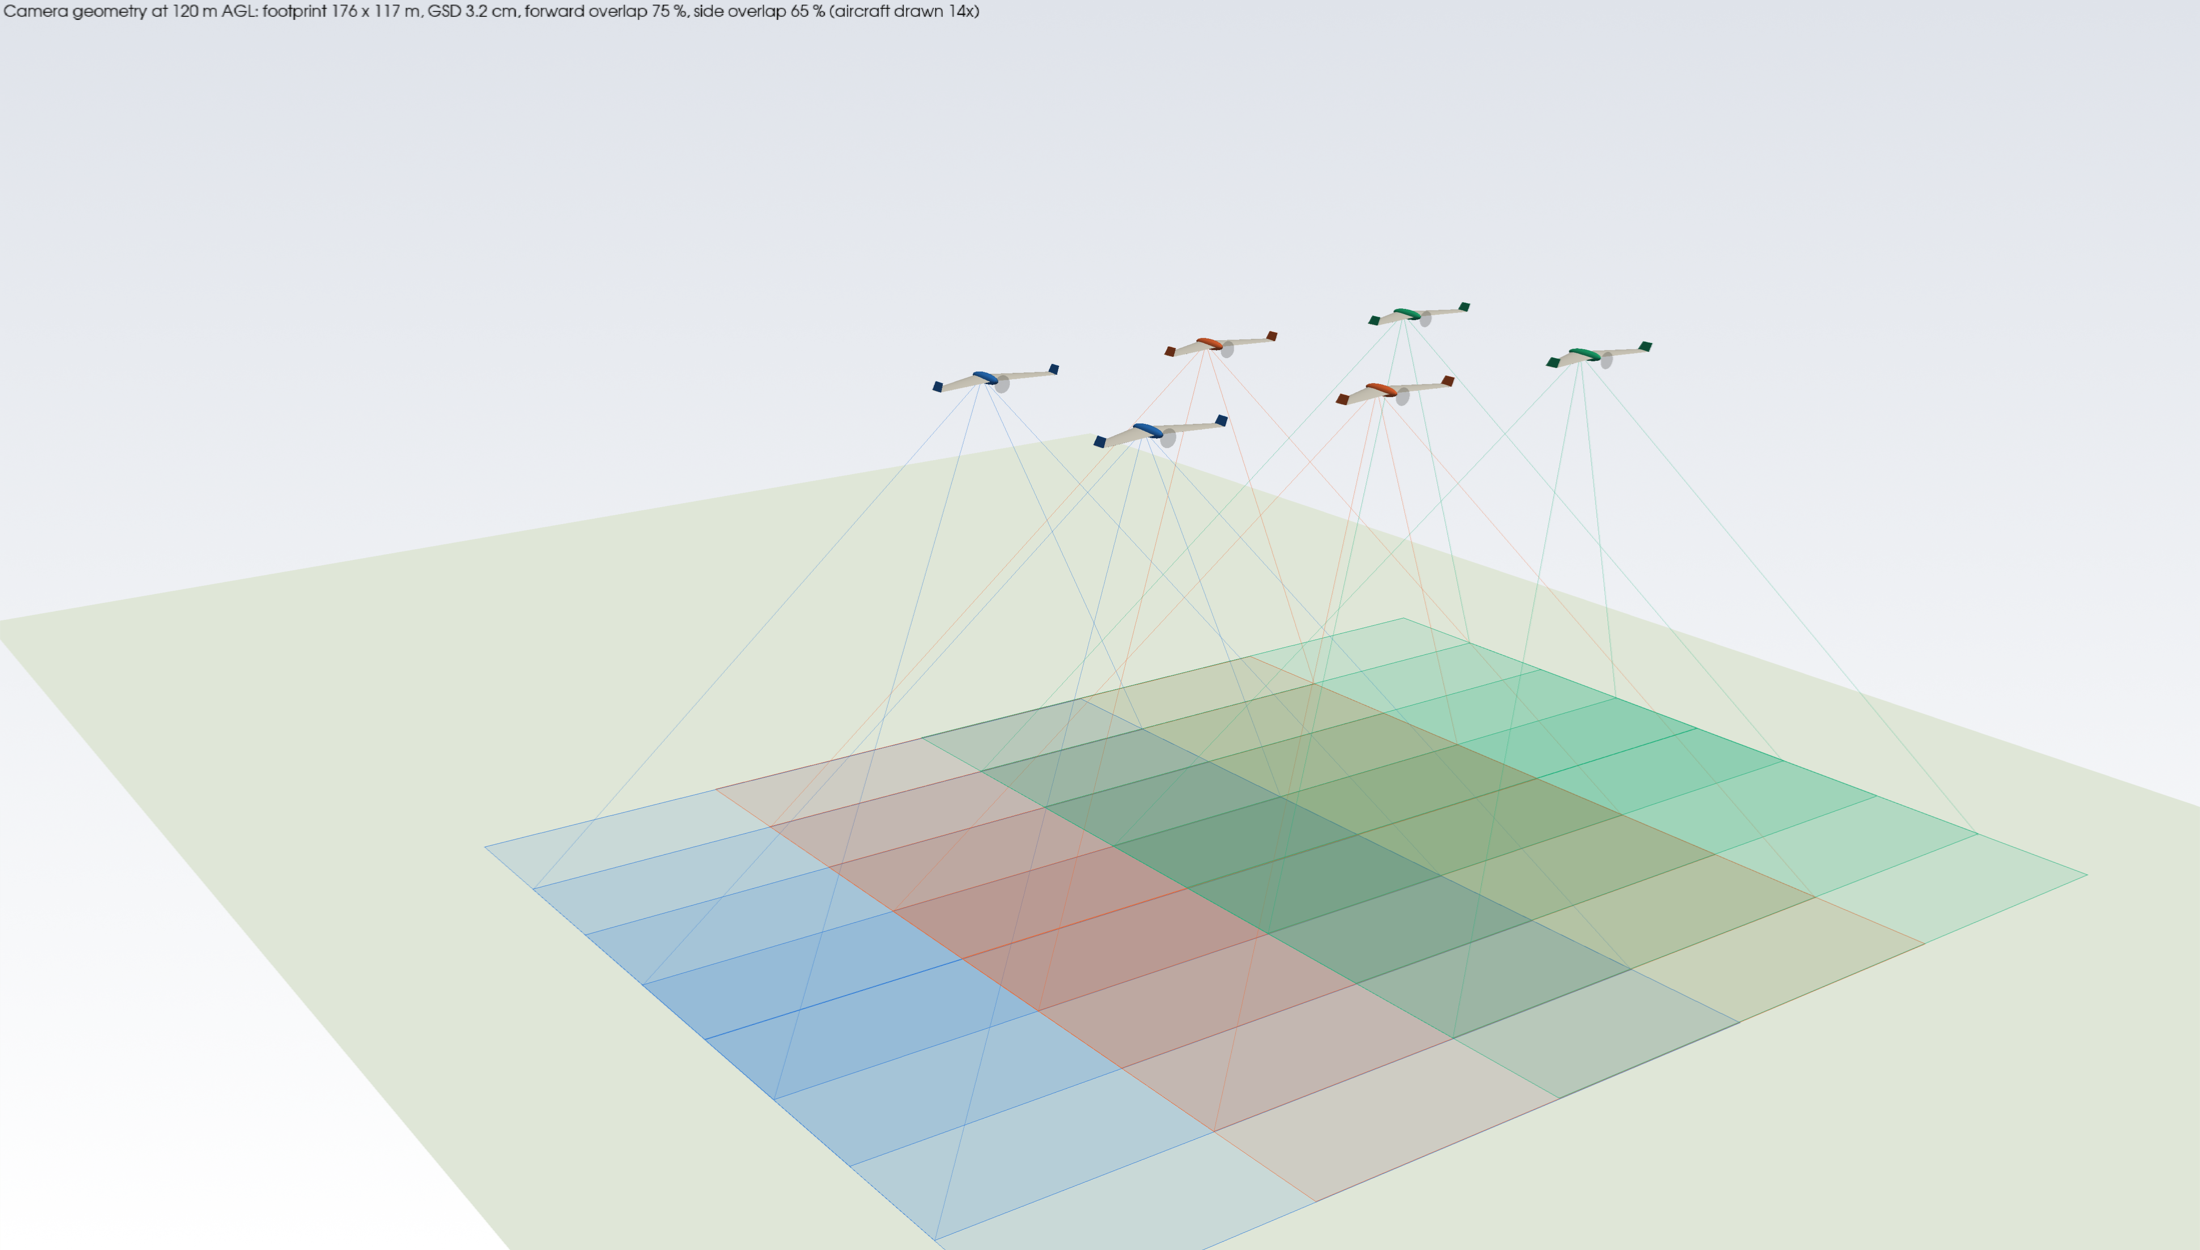
\includegraphics[width=\textwidth]{C1_camera_frustums}
\caption{True camera geometry for three adjacent strips at \SI{120}{m} AGL: footprints, 75\,\% forward and 65\,\% side overlap, GSD \SI{\ngsd}{cm}.}\label{fig:C1}\end{figure}
\begin{figure}[H]\centering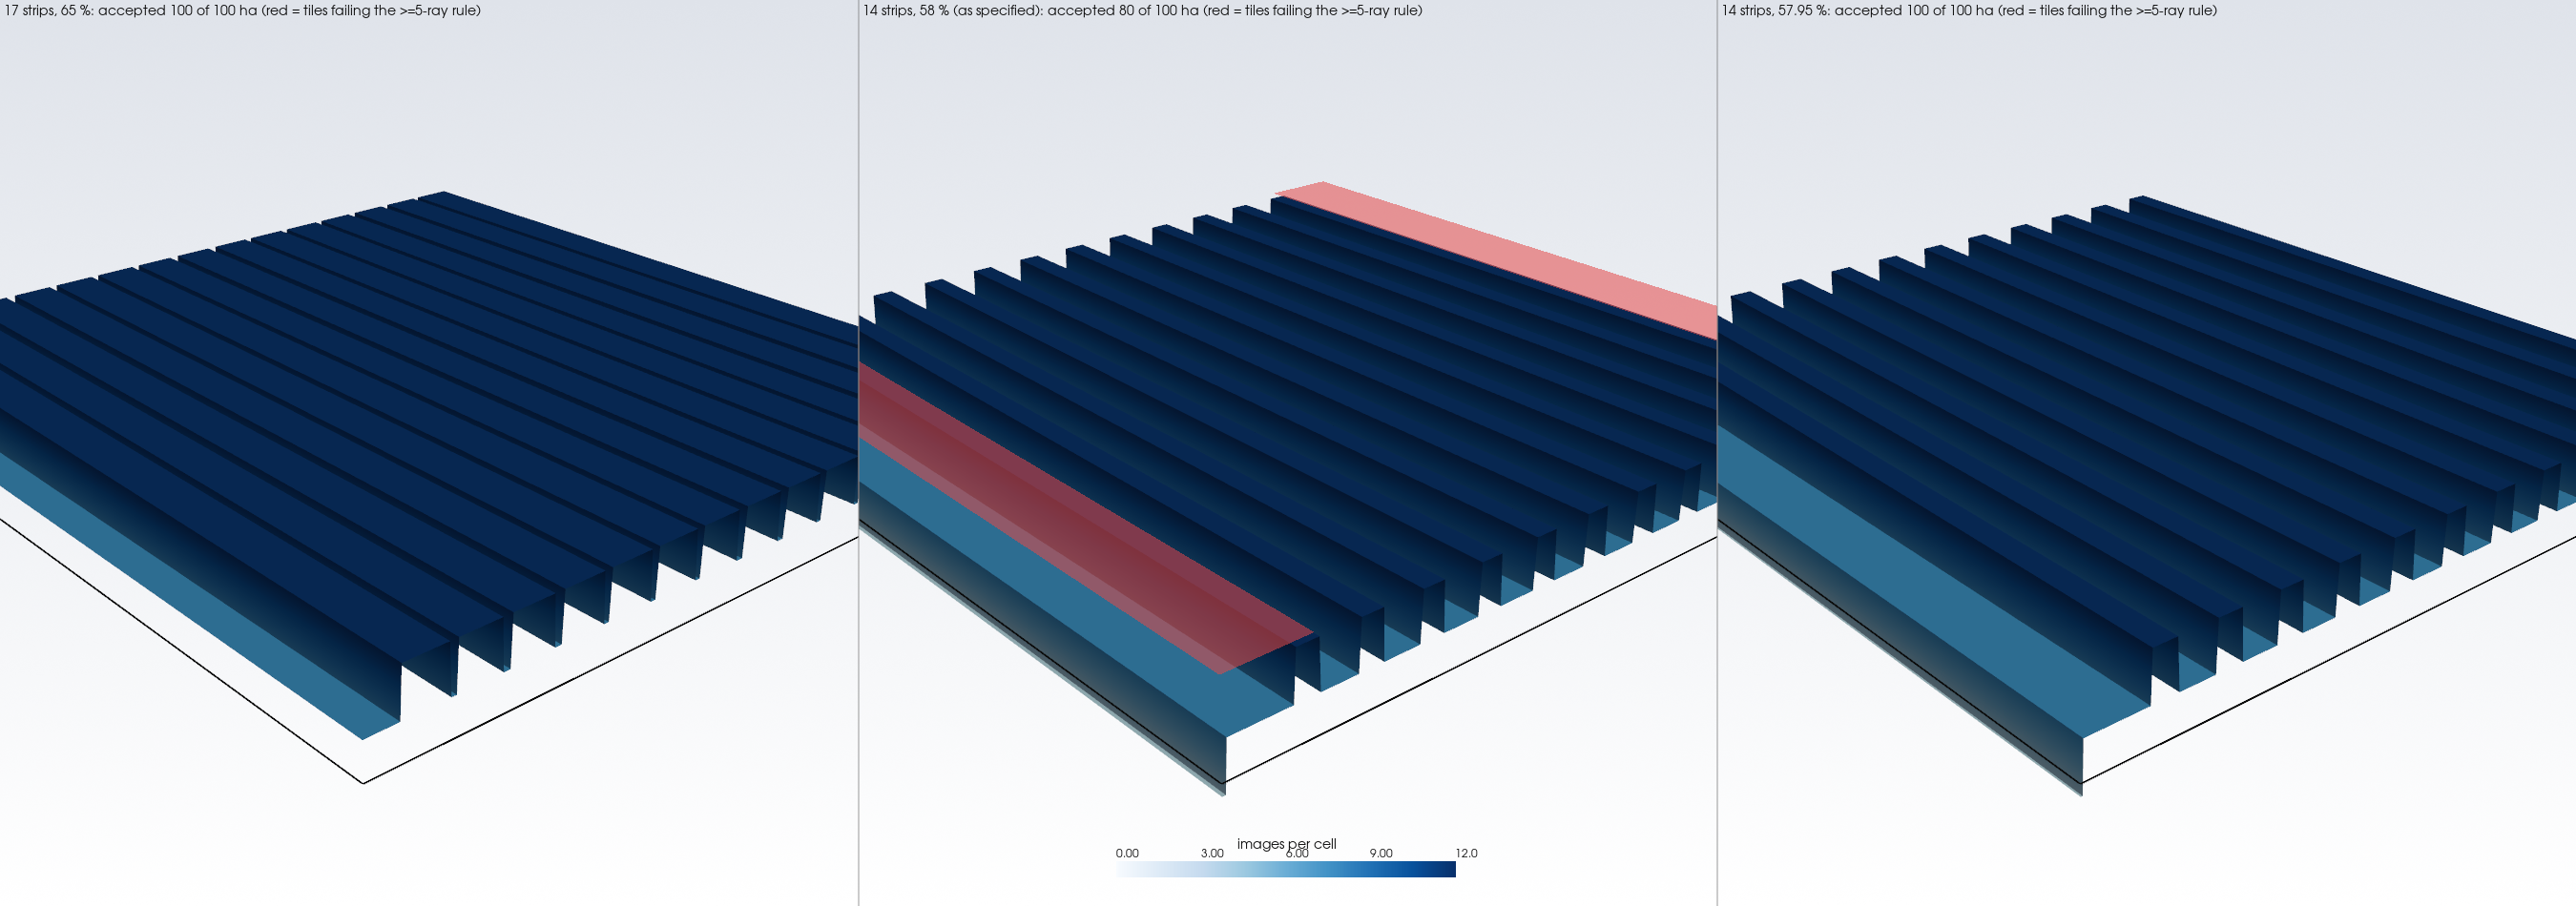
\includegraphics[width=\textwidth]{C2_coverage_relief}
\caption{Ray multiplicity as relief for the three route plans; red tiles fail the $\ge5$-ray rule at the block edge (\SI{80}{ha} accepted for the 14-strip plan at the specified \SI{58}{\percent}).}\label{fig:C2}\end{figure}
\begin{figure}[H]\centering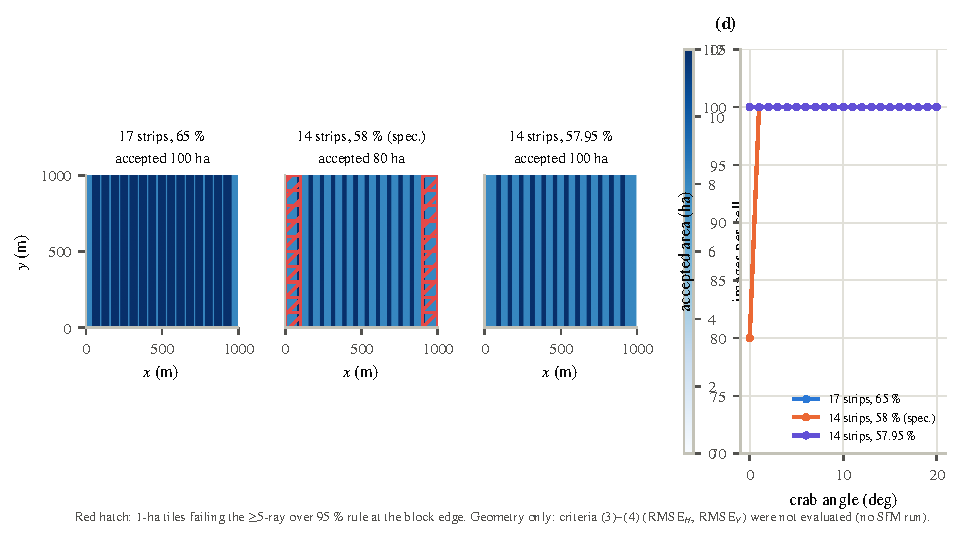
\includegraphics[width=\textwidth]{fig13_mapping_geometry}
\caption{Ray multiplicity for the three route plans and accepted area vs.\ camera crab angle. Geometry only; no SfM was run.}\label{fig:map13}\end{figure}
The 17-strip plan has a minimum multiplicity of \nminMultSeven{} (mean \nmeanMultSeven). The 14-strip plan at the claimed \SI{58}{\percent} overlap has a minimum of \nminMultFourteen{} and, with the strip block centred and zero crab, the outer 1-ha columns fail the five-ray criterion over \SI{95}{\percent} of the tile by a margin of \nedgeFailM\,m (accepted area \naccFourteen\,ha). Any crab angle above about \SI{1}{\degree} (wind $>0.3$ m/s) widens the rotated footprint enough to pass, and a spacing of \SI{74.0}{m} (\nMarginOverlap\,\% overlap) passes at zero crab; we use the latter in S4. The 58\,\% plan therefore sits within a fraction of a percent of violating the preliminary version's own acceptance rule. The base-to-height ratio between adjacent strips rises from \nBHbase{} to \nBHopt{}, which favours intersection geometry in principle, but whether tie-point density and RTK-constrained bundle adjustment maintain RMSE$_H\le\SI{4.5}{cm}$ and RMSE$_V\le\SI{6.5}{cm}$ cannot be answered without reconstruction: no accuracy claim is made, and the preliminary RMSE tables are withdrawn (\ref{app:audit}). Independent aircraft carrying RTK receivers could in principle use the same 58\,\% plan; the claim that it needs synchronised formation flight is untested.

\subsubsection{Overlap sweep and acceptance margin}
Figure~\ref{fig:X5} sweeps the side overlap from 50 to 70\,\% with the strip count and spacing recomputed at each value and the block centred in the polygon. At zero crab the accepted area equals the full \SI{100}{ha} only for side overlaps up to about \ncovMinOverlap\,\% and again at isolated higher values; around the claimed \SI{58}{\percent} the five-ray rule fails at the block edge for several consecutive overlaps (failing values include \ncovFailWindow\,\%). The number of strips steps from \ncovStripsSixFive{} at 65\,\% to \ncovStripsFiveEight{} at 58\,\%, saving \ncovTrackSave\,km of track. Crab angle changes the picture because the rotated footprint widens the cross-track extent: with crab $\ge3^\circ$ the failing window shrinks and with $\ge6^\circ$ it disappears, i.e.\ the acceptance of the 58\,\% plan depends on the wind---a fragility that a planner must treat as a constraint, not an average. The base-to-height ratio between adjacent strips grows linearly as overlap decreases, from \nBHbase{} at 65\,\% to \nBHopt{} at 58\,\%, which strengthens the intersection geometry between strips but, as stated above, says nothing about tie-point density.
\begin{figure}[H]\centering\includegraphics[width=\textwidth]{X5_overlap_sweep}
\caption{(a) Geometrically accepted area versus side overlap for five camera crab angles; (b) strips needed to cover \SI{1}{km}; (c) base-to-height ratio and minimum number of covering images (divided by 10).}\label{fig:X5}\end{figure}


\subsection{OpenFOAM RANS verification of the wake model}\label{sec:cfd}

The vortex-lattice and free-wake models are inviscid and are cross-checked against each other, not against a viscous solution. This section compares them with Reynolds-averaged simulations of the same planform (Sec.~\ref{sec:cfdsetup}) at $U_\infty=\SI{18}{m/s}$ ($Re_{\mathrm{MAC}}=\nReMAC$). Every case in Table~\ref{tab:cfdcases} was run to completion; the table lists all 13 cases without exclusion. Forces are integrated in Python from the exported patch fields (Sec.~\ref{sec:cfdsetup}), and the leader loads are doubled for the half-model.

\begin{table}[H]\centering\scriptsize\caption{All OpenFOAM cases (leader quantities are full-aircraft values; follower columns are given when a follower is present). $y^+$ is the mean wall-function $y^+$ on the leader; iterations are SIMPLE iterations to the residual-control stop (cap 700).}\label{tab:cfdcases}

\resizebox{\textwidth}{!}{\begin{tabular}{@{}lrrrrrrrrr@{}}\toprule Case & cells (k) & $\alpha$ & $C_L$ & $C_D{\times}10^4$ & $y^+$ & $C_L^{F}$ & $C_D^{F}{\times}10^4$ & iter. & solve (min)\\\midrule

iso\_a0\_L1 & 381 & 0 & -0.0139 & 90.3 & 61 & -- & -- & 368 & 2.0 \\
iso\_a3\_L0 & 82 & 3 & 0.2119 & 218.3 & 87 & -- & -- & 366 & 0.5 \\
iso\_a3\_L1 & 381 & 3 & 0.2178 & 153.1 & 61 & -- & -- & 370 & 2.1 \\
iso\_a3\_L2 & 1251 & 3 & 0.2223 & 123.8 & 51 & -- & -- & 400 & 9.0 \\
iso\_a6\_L1 & 378 & 6 & 0.4115 & 329.7 & 58 & -- & -- & 346 & 2.2 \\
fol\_dy070\_dx3\_L1 & 735 & 3 & 0.2263 & 156.0 & 61 & 0.2479 & 150.8 & 354 & 4.5 \\
fol\_dy085\_dx2\_L1 & 666 & 3 & 0.2253 & 155.4 & 61 & 0.2517 & 151.5 & 344 & 3.7 \\
fol\_dy085\_dx3\_L0 & 155 & 3 & 0.2083 & 216.7 & 88 & 0.2322 & 223.5 & 374 & 0.9 \\
fol\_dy085\_dx3\_L1 & 749 & 3 & 0.2263 & 155.9 & 61 & 0.2519 & 151.1 & 356 & 4.4 \\
fol\_dy085\_dx3\_L2 & 3611 & 3 & 0.2219 & 123.5 & 51 & 0.2549 & 119.5 & 398 & 27.3 \\
fol\_dy085\_dx45\_L1 & 861 & 3 & 0.2190 & 154.2 & 61 & 0.2482 & 151.6 & 366 & 4.0 \\
fol\_dy100\_dx3\_L1 & 780 & 3 & 0.2263 & 155.9 & 61 & 0.2499 & 153.1 & 354 & 4.7 \\
fol\_dy130\_dx3\_L1 & 857 & 3 & 0.2262 & 155.9 & 61 & 0.2340 & 154.1 & 362 & 5.5
\\\bottomrule\end{tabular}}\end{table}

Mesh dependence of the isolated wing at $\alpha=3^\circ$ (Fig.~\ref{fig:CF1}): going from L0 (82k cells) to L1 (381k) changes $C_L$ by +2.8\,\% and $C_D$ by -29.9\,\%; from L1 to L2 (1251k) the changes are +2.1\,\% in $C_L$ and -19.2\,\% in $C_D$; the Richardson extrapolation of $C_{L}$ is 0.2398 (observed order 0.6); the Richardson extrapolation of $C_{D}$ is 0.0095 (observed order 1.8). The mean $y^+$ falls from 87 to 61 and 51, inside the wall-function range (30--300) for L1 and L2 but marginal for L0, so the L0 drag is not credible (the viscous drag is under-predicted by 44\,\% relative to L1). The absolute drag is therefore \emph{not} mesh-converged: it is still falling by about a fifth between L1 and L2, with the pressure part decreasing and the viscous part increasing as the wall resolution improves, and the lift is still moving by about 2\,\%. Absolute RANS drag values in this section are consequently indicative only; the comparisons that follow use differences between flows on the same mesh family.

\begin{figure}[H]\centering\includegraphics[width=\textwidth]{C1_mesh_study}\caption{Mesh study: (a) lift coefficient, (b) drag coefficient with pressure and viscous parts, (c) wall-function $y^+$ (mean and 5--95\,\% range) for the isolated wing and, where available, the follower at $d_y=0.85b$, $d_x=3b$.}\label{fig:CF1}\end{figure}

\paragraph{Polar} Figure~\ref{fig:CF2} compares the L1 RANS polar with the planform VLM. The RANS lift-curve slope between $0^\circ$ and $6^\circ$ is 4.06\,rad$^{-1}$ against \nplanCla\,rad$^{-1}$ from the planform VLM (-2\,\%). The RANS drag rises much faster with lift than the inviscid induced drag: the quadratic fit gives $C_{D0}=0.0088$ and $k=0.142$ versus $k_{\mathrm{VLM}}=0.054$, i.e.\ an apparent span efficiency of 0.41. The excess is profile and pressure drag growth on the unrefined, boundary-layer-free mesh and is the reason why the absolute RANS drag cannot be compared with the empirical $C_{D0}=0.024$ of the system model; only \emph{differences} between flows on identical meshes are used below.

\begin{figure}[H]\centering\includegraphics[width=\textwidth]{C2_polar_cfd_vs_vlm}\caption{Isolated-wing polar: (a) $C_L(\alpha)$, (b) drag polar, (c) $C_D$ versus $C_L^2$ with the linear fit used to extract $C_{D0}$ and $k$. RANS at mesh level L1.}\label{fig:CF2}\end{figure}

\paragraph{Wake of the isolated wing} Figure~\ref{fig:CF3} shows the vertical-velocity field of the leader's wake at $x=3b$ from the L1 solution. A tip vortex dipole is clearly resolved: downwash inboard of the tip and an upwash peak of about 4.5\,\% of $U_\infty$ at $y\approx0.52b$, decaying slowly outboard. This is the same structure and sign that the free-wake solver predicts at this distance, where the wake is bowed but not rolled up into a concentrated pair, and it is the mechanism that gives the lateral breadth of the follower benefit. The resolved peak is limited by the numerical diffusion of the L1 wake box (level 3, cells of order $0.06$\,m, to be compared with a physical core radius of a few centimetres); a finer wake box would sharpen the peak and shift the best offset slightly outboard.

\begin{figure}[H]\centering\includegraphics[width=\textwidth]{C3_wake_plane_cfd}\caption{RANS vertical velocity in the plane $x=3b$ downstream of the isolated leader (half-model, $y\ge0$): (a) $w/U_\infty$ field; (b) profile at $z\approx0$.}\label{fig:CF3}\end{figure}

\paragraph{Follower in the wake} Table~\ref{tab:cfdformation} and Fig.~\ref{fig:CF4} give the follower's loads relative to the isolated wing on the same mesh family, at fixed angle of attack ($\alpha=3^\circ$). At $d_y=0.85b$, $d_x=3b$ the follower lift rises by $\Delta C_L=+0.0341$ (VLM: +0.0320) and its drag changes by $\Delta C_D=-2.0\times10^{-4}$ (VLM, induced part: -14.3$\times10^{-4}$). The lift response, a measure of the mean upwash the follower sees, agrees with the VLM within 7\,\% at this offset; at $0.7b$ and $1.3b$ the RANS increment is larger than the VLM's (by 49 and 62\,\%), i.e.\ the RANS upwash field is broader laterally than the planar sheet.

A fixed-angle comparison understates the energy benefit, because a follower at constant weight must \emph{reduce} its angle of attack to remove the extra lift. Trimming back to the isolated lift with the polar slope $\mathrm{d}C_D/\mathrm{d}C_L$ of the \emph{inviscid} model (0.023) gives a drag reduction of $-6.5$\,\% of the follower's total RANS drag at $d_y=0.85b$ against $14.2$\,\% for the VLM; trimming with the (much steeper, partly viscous) RANS slope (0.062) would give -15.1\,\%. Expressed as an effective wake effectiveness $\kappa_{\mathrm{eff}}$ (the factor by which the VLM benefit must be multiplied to match the RANS result) the two trimming choices bracket 0.46--1.06 at $0.85b$; the lower value (inviscid slope) is the better-defined one because the steep RANS slope contains profile-drag growth that is not a wake effect. The mission model already carries $\kappa\in[0.3,1.5]$ (Sec.~\ref{sec:sens}), so the RANS results fall inside the explored sensitivity range; their central estimate ($\kappa_{\mathrm{eff}}\approx0.4$--$0.6$ over $0.7b$--$1.0b$) is below the planar-sheet value and also below the free-wake-to-sheet benefit ratio of about 0.7. The RANS and VLM agree on the lateral shape: the benefit is broad between $0.7b$ and $1.0b$ and has fallen by two thirds at $1.3b$ (Fig.~\ref{fig:CF4}).

\begin{table}[H]\centering\scriptsize\caption{Follower effect relative to the isolated wing (RANS L1 versus planform VLM, $\alpha=3^\circ$). $\Delta C_D$ columns are $\times10^{-4}$; the trimmed saving is the drag change at the isolated lift, as a percentage of the isolated RANS drag (RANS rows trimmed with the inviscid slope, see text; VLM rows use the same $C_D$ denominator). $\kappa_{\mathrm{eff}}$ brackets the ratio of the RANS to the VLM trimmed saving.}\label{tab:cfdformation}

\resizebox{\textwidth}{!}{\begin{tabular}{@{}rrrrrrrrr@{}}\toprule $d_x/b$ & $d_y/b$ & $\Delta C_L$ RANS & $\Delta C_L$ VLM & $\Delta C_D$ RANS & $\Delta C_{D,i}$ VLM & trimmed RANS (\%) & trimmed VLM (\%) & $\kappa_{\mathrm{eff}}$\\\midrule

2.0 & 0.85 & +0.0339 & +0.0317 & -1.6 & -14.1 & -6.2 & -14.0 & 0.44--1.05 \\
3.0 & 0.70 & +0.0301 & +0.0202 & -2.3 & -11.2 & -6.1 & -10.4 & 0.59--1.32 \\
3.0 & 0.85 & +0.0341 & +0.0320 & -2.0 & -14.3 & -6.5 & -14.2 & 0.46--1.06 \\
3.0 & 1.00 & +0.0321 & +0.0304 & -0.0 & -12.8 & -4.9 & -13.0 & 0.38--1.00 \\
3.0 & 1.30 & +0.0162 & +0.0100 & +1.0 & -3.1 & -1.8 & -3.6 & 0.51--1.66 \\
4.5 & 0.85 & +0.0304 & +0.0322 & -1.5 & -14.4 & -5.6 & -14.3 & 0.39--0.93
\\\bottomrule\end{tabular}}\end{table}

\begin{figure}[H]\centering\includegraphics[width=\textwidth]{C4_formation_cfd_vs_vlm}\caption{Follower response versus lateral offset for three streamwise distances: (a) drag change at fixed angle of attack, (b) lift change, (c) roll-moment coefficient (RANS markers, VLM lines).}\label{fig:CF4}\end{figure}

\paragraph{Streamwise distance} At $d_y=0.85b$ the lift increment is +0.0339 at $d_x=2.0b$ (VLM +0.0317), +0.0341 at $d_x=3.0b$ (VLM +0.0320), +0.0304 at $d_x=4.5b$ (VLM +0.0322), and the trimmed saving (inviscid slope) is -6.2\,\% at $2.0b$, -6.5\,\% at $3.0b$, -5.6\,\% at $4.5b$. The weak dependence on $d_x$ confirms that, within the first five spans, the benefit is controlled by lateral rather than longitudinal position.

\paragraph{Roll moment} The RANS rolling-moment coefficient of the follower at $0.85b$ is -0.0020 (VLM -0.0024): the sign matches the VLM at all four offsets (positive at $0.7b$, negative at $0.85b$, $1.0b$ and $1.3b$), with magnitudes $|C_l|=0.001$--$0.0035$ against an elevon authority $C_{l\delta a}\delta_{\max}\approx0.05$ for an assumed $\delta_{\max}=20^\circ$; the wake-induced roll moment is therefore a few per cent of the control authority, consistent with treating it as a bounded disturbance in the control model (the $\sim$50\,\% magnitude differences with the VLM are within what a one-sided surface integration of a small moment on this mesh can resolve).

\paragraph{Mesh sensitivity of the follower effect} Repeating the isolated and follower cases at level L2 (1251k and 3611k cells) changes the lift increment from +0.0341 to +0.0325 (5\,\%) but the drag increment from -2.0 to -4.2 ($\times10^{-4}$), i.e.\ it roughly doubles. The drag increment is therefore itself mesh-sensitive, as expected for a pressure-integrated RANS drag that is not mesh-converged (the L1 to L2 change in the isolated $C_D$ is -19.2\,\%). With the inviscid trimming slope the finer mesh gives $\kappa_{\mathrm{eff}}=0.54$ at $0.85b$ against 0.46 at L1, so the central estimate moves towards, but stays below, the planar-sheet value; the drag-based $\kappa_{\mathrm{eff}}$ should be read as an order-of-magnitude confirmation, not a calibration.

\paragraph{Flow visualisation} Figures~\ref{fig:K1}--\ref{fig:K3} show the solution in three dimensions: the surface pressure on the three aircraft, the vortex system and the vertical-velocity planes. The follower sits in the outboard upwash of the leader's tip vortex, and the isolated-wing pressure distribution shows the expected suction peak on the forward upper surface.

\begin{figure}[H]\centering\includegraphics[width=\textwidth]{K1_cp_fol_dy085_dx3_L1}\caption{Surface pressure coefficient on the leader (mirrored through the symmetry plane) and the two followers at $d_x=3b$, $d_y=0.85b$ (RANS, L1).}\label{fig:K1}\end{figure}

\begin{figure}[H]\centering\includegraphics[width=\textwidth]{K2_vortex_fol_dy085_dx3_L1}\caption{Iso-surface of the Q-criterion ($Q=0.1\,(U_\infty/b)^2$) coloured by streamwise vorticity, with the wall region masked, for the formation case.}\label{fig:K2}\end{figure}

\begin{figure}[H]\centering\includegraphics[width=\textwidth]{K3_wslices_fol_dy085_dx3_L1}\caption{Vertical velocity $w/U_\infty$ on four cross-flow planes ($x=1$\,m, $3b$, $5b$, $8b$): the leader's tip upwash decays and diffuses; the follower's own wake appears at $x=5b$ and beyond.}\label{fig:K3}\end{figure}

\begin{figure}[H]\centering\includegraphics[width=\textwidth]{C6_residual_history}\caption{Initial-residual histories of the L1 isolated and follower cases; both stop on the residual-control criterion before the iteration cap.}\label{fig:CF6}\end{figure}

\paragraph{What the CFD does and does not show} The RANS results (i) confirm the sign, order of magnitude and lateral breadth of the wake benefit, (ii) show that the lift (upwash) response is predicted by the planar-sheet VLM within about 7\,\% at the best offset (RANS broader laterally), (iii) bracket the \emph{drag} benefit at roughly $0.4$ to $1.1$ times the VLM value at $0.85b$--$1.0b$, and (iv) provide no support for benefits larger than the VLM predicts. They do \emph{not} validate the model quantitatively: the geometry is a clean wing without fuselage, propeller or control surfaces, the mesh has no prism layers, wall functions are used at $y^+\approx60$, the flow is steady RANS (no turbulence in the free stream, no wake meander), the drag is obtained by surface integration with a Python post-processor, and no experimental data for this planform exist for comparison. The mission-level conclusions of Sec.~\ref{sec:mission} are therefore unchanged: the CFD stays within the sensitivity range already explored.


%==============================================================================================
\section{Discussion and limitations}
\paragraph{What the evidence supports} (1) A rigid V is unsuitable for nadir mapping (\nrelCSheet\,\% energy). (2) Corrected physics gives a broad \npeakFree--\npeakSheet\,\% follower-power benefit near $0.85$--$0.90b$ at \SI{18}{m/s}, rising at lower speed, consistent between the free-wake simulation, an independent VLM and corrected strip theory and bracketed by steady RANS CFD at 0.4--1.1 times the planar-sheet value but unvalidated against measurement; the wake is not rolled up at the formation distance. (3) For a \SI{2.5}{km} transit, adaptive formation is a net loss; break-even is at roughly \nbeSevSheet--\nbeSevFree\,km one-way in this model, dominated by distance. (4) The apparent mission gain of the full framework is attributable to route/overlap planning under an unverified overlap assumption. (5) A barrier-function filter does not remove the need for authority margins.

\paragraph{Limitations} The wake models are inviscid: the free wake resolves sheet sinking and the onset of roll-up but its core radius is prescribed (not calibrated), and there is no turbulence, atmospheric stratification, wake meander or aircraft-to-wake feedback. The aircraft is a rectangular-equivalent wing; $C_{D0}$, $e_0$, $\eta_p$, hotel load, trim-drag law and elevon effectiveness come from the preliminary version. The control simulation is a guidance-level point mass with kinematic wind, no wake-to-dynamics feedback, no altitude channel, and a single 2-D formation plane. Battery parameters are generic. Terrain is flat; photogrammetric accuracy was not computed. The statistical design samples only environmental and station-keeping variability, so narrow trial intervals reflect simulator determinism, not confidence about reality; model-form spread (Table~\ref{tab:paired}) is the more honest uncertainty.

\paragraph{Decision rule for practitioners} The model-based break-even gives a simple rule: formation transit pays only if the one-way transit exceeds roughly the distance at which the cumulative wake saving (follower saving $\times$ time at the slot) exceeds the fixed reconfiguration and formation-assembly cost (Sec.~\ref{sec:reconf}); with $\kappa\in[0.3,1.5]$ this distance spans several kilometres (Fig.~\ref{fig:X2}), so for single-block surveys within a few kilometres of the launch point independent flight on the optimised route is preferable. Formation becomes attractive for long ferry legs, repeated blocks, or when the fleet must in any case travel together.

\paragraph{Threats to validity} \emph{Internal:} all aerodynamic inputs outside the wake ($C_{D0}$, $e_0$, $\eta_p$) are inherited and unverified; the NMPC is a point-mass abstraction. \emph{Construct:} energy per accepted hectare depends on an acceptance rule (five-ray multiplicity) that is a geometric proxy for photogrammetric success. \emph{External:} one aircraft class, one wind distribution, flat terrain, one block geometry. \emph{Conclusion:} the narrow trial-wise intervals are properties of a near-deterministic simulator; model-form spread and the $\kappa$ sensitivity are the relevant uncertainty.

\paragraph{Relation to the literature} The follower benefit we obtain is smaller than the quarter-scale lift-to-drag gains reported for close-formation CFD at higher lift coefficients \cite{oendo2025} because a survey cruise operates at $C_L\approx0.22$ where induced drag is a small fraction of the total; the RANS follower response (lift increase of about 0.03 and a trimmed drag reduction of roughly 6--15\,\% of the total RANS drag, depending on the trimming slope) is of the same sign and order as ideal-aerodynamics predictions \cite{king2005,katz2001}.

\paragraph{Next validation steps} (i) higher-fidelity CFD (prism layers, URANS or scale-resolving, propeller and fuselage) with a published benchmark and wind-tunnel data for this planform; (ii) 6-DOF SITL with the wake-force plugin and the same scenarios; (iii) controlled comparison of $65\%$ vs.\ $58\%$ side overlap for \emph{single} and \emph{formation} acquisition on a surveyed test range with independent checkpoints; (iv) flight test of a two-aircraft formation with measured electrical power at stepped offsets and altitudes.

\section{Conclusions}
Within a transparent and reproducible simulation, wake-aware formation flight with a three-aircraft survey fleet does not lower energy per accepted hectare at a \SI{2.5}{km} transit; the apparent \nabsASheet\,\% saving of the complete framework derives from a shorter route enabled by a relaxed overlap assumption that is not yet verified and not specific to formation. The wake saving is real in the model but modest (\npeakFree--\npeakSheet\,\% of power per follower), broad in lateral offset, and pays off only for transits beyond roughly \nbeSevSheet--\nbeSevFree\,km one-way. Steady RANS CFD of the planform supports the existence and lateral breadth of the wake benefit and places its magnitude at 0.4--1.1 times the planar-sheet value, inside the sensitivity range used for the mission results. Claims about photogrammetric accuracy, experimental agreement and in-flight safety require the validation steps above.

%==============================================================================================
\section*{Declarations}
\textbf{CRediT:} [to be completed by the authors]. \textbf{Competing interests:} [to be completed]. \textbf{Funding:} [to be completed]. \textbf{Use of AI assistance:} code, analysis scripts and a first draft of this manuscript were produced with an AI coding assistant working from the authors' preliminary manuscript and a reviewer's assessment; the authors remain responsible for verifying all content. \textbf{Data and code availability:} all scripts, raw trial data (control and mission), processed tables and figure sources are in the repository accompanying this submission (\texttt{flockmap-research/}); a persistent archive (DOI) is to be created on acceptance. No external datasets were used.

\appendix
\setcounter{figure}{0}\setcounter{table}{0}
\section{Audit of the preliminary version}\label{app:audit}
The preliminary version's numerical sections (aerodynamics table, Sec.~6.2 code, Sec.~7 statistics) were re-derived. Findings, each reproduced by \texttt{audit/} and \texttt{tests/}:
\begin{enumerate}\small
\item \textbf{Circulation} $\Gamma_0=4VSC_L/(\pi b)$ is twice $L/(\rho Vb_0)$ (\ngammaPub{} vs.\ \ngammaTrue\,m$^2$/s).
\item \textbf{Roll moment} used $1/(bS)$ (not dimensionless) and lift slope $2\pi$: $C_{l,\mathrm{wake}}$ overstated by \nclPubOverCorr$\times$ at $0.8b$; trim-drag penalties ($\propto C_l^2$) overstated by an order of magnitude.
\item \textbf{Table not reproducible:} the published equations reproduce the printed upwash for only \nnTabMatch{} of \nnTabAll{} lateral offsets; at $0.85$, $0.90$ and $1.0b$ the code gives \npubAtEightyFive, \npubDropNinety\,\% and negative savings where the table prints $+5.95$, $+5.06$, $+3.62$\,\% (max.\ discrepancy \nauditMaxPctErr\,percentage points; Fig.~\ref{fig:A1}, Table~\ref{tab:audit}).
\item \textbf{Synthetic outcomes:} horizontal/vertical RMSE and accepted-area fractions were drawn from \texttt{np.random.normal/uniform} with the means printed in the results table; they are not measurements.
\item \textbf{Degenerate statistics:} all energy variance came from one scalar draw shared by all UAVs and strategies (correlation between strategies \nauditCorr), so reproducing the code gives $|t|\approx\nauditHthreeT$ and $|d_z|\approx\nauditHthreeD$ for the H$_3$ comparison. These are artefacts, not evidence. The reported standard deviations (e.g.\ \SI{1.15}{Wh} for S1) are also smaller than the code generates (\nauditEoneSD\,Wh).
\item \textbf{Wind unused:} wind speed/direction were stated but no wind enters the energy calculation; climb, landing, reserve, battery sag, waiting and ferry legs were absent; strips 61.6\,m apart were joined by 222.6\,m semicircles although the turn diameter is 141.7\,m.
\item \textbf{Reconfiguration cost} double-counted flight time (full cruise power for 45\,s added to time already integrated).
\item \textbf{HOCBF relative degree} was stated as 2; with the stated bank-lag dynamics it is 3.
\item \textbf{Turn power:} \SI{146.42}{W} at $25^\circ$ bank is inconsistent with the stated polar (\SI{\npTurn}{W}).
\end{enumerate}
\begin{figure}[H]\centering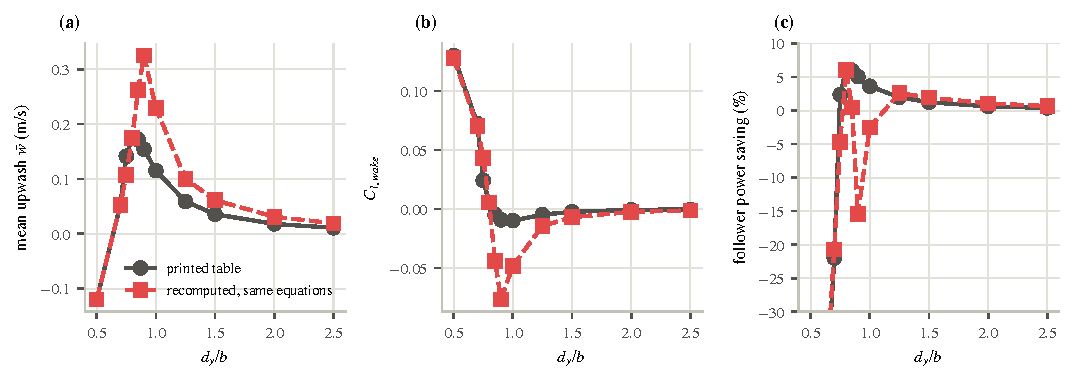
\includegraphics[width=\textwidth]{figA1_table_audit}
\caption{Printed table of the preliminary version versus the same equations recomputed.}\label{fig:A1}\end{figure}
\begin{table}[H]\centering\scriptsize
\caption{Printed vs.\ recomputed values (published equations, $d_x=3b$).}\label{tab:audit}
\begin{tabular}{@{}rrrrrrr@{}}\toprule $d_y/b$ & $\bar w$ table & $\bar w$ recomp. & $C_l$ table & $C_l$ recomp. & $\%P$ table & $\%P$ recomp.\\\midrule
0.50 & -0.1200 & -0.1200 & +0.1298 & +0.1278 & -81.38 & -79.04 \\
0.70 & +0.0526 & +0.0526 & +0.0722 & +0.0702 & -22.00 & -20.70 \\
0.75 & +0.1412 & +0.1069 & +0.0241 & +0.0431 & +2.35 & -4.73 \\
0.80 & +0.1748 & +0.1748 & +0.0054 & +0.0054 & +6.05 & +6.05 \\
0.85 & +0.1715 & +0.2623 & -0.0048 & -0.0439 & +5.95 & +0.46 \\
0.90 & +0.1541 & +0.3246 & -0.0092 & -0.0767 & +5.06 & -15.46 \\
1.00 & +0.1149 & +0.2292 & -0.0098 & -0.0482 & +3.62 & -2.51 \\
1.25 & +0.0588 & +0.1002 & -0.0049 & -0.0145 & +1.97 & +2.58 \\
1.50 & +0.0355 & +0.0610 & -0.0024 & -0.0069 & +1.24 & +1.94 \\
2.00 & +0.0178 & +0.0309 & -0.0008 & -0.0025 & +0.62 & +1.06 \\
2.50 & +0.0108 & +0.0189 & -0.0004 & -0.0012 & +0.39 & +0.66
\\
\bottomrule\end{tabular}\end{table}
\begin{figure}[H]\centering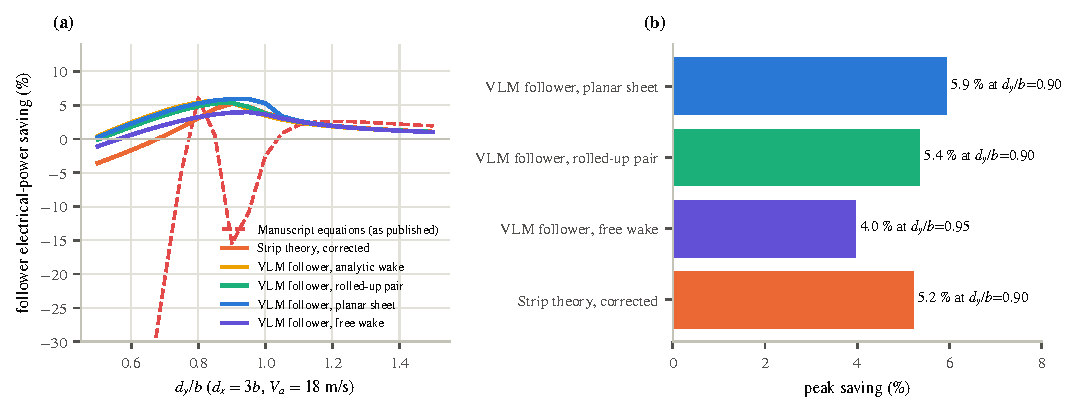
\includegraphics[width=\textwidth]{figA2_model_comparison}
\caption{Follower power saving for the published equations and four corrected/independent variants; (b) peak saving per model.}\label{fig:A2}\end{figure}
\begin{figure}[H]\centering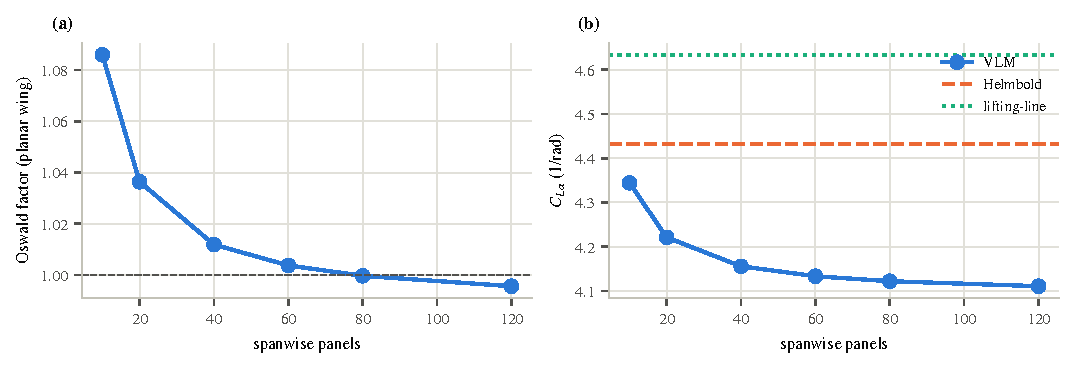
\includegraphics[width=0.85\textwidth]{figA3_vlm_verification}
\caption{Vortex-lattice verification: (a) Oswald factor and (b) lift slope versus panel count.}\label{fig:A3}\end{figure}

\section{Parameter register}\label{app:params}
Every numerical input carries a provenance tag: \textbf{MS} -- taken from the preliminary manuscript and not independently re-measured on a specific test airframe (baseline aerodynamic values are cross-checked against published Skywalker-X8 wind-tunnel and flight-identification ranges \cite{gryte2018,reinhardt2022}); \textbf{DER} -- derived from other parameters; \textbf{ASM} -- an assumption introduced in this study that must be replaced by measurement. Values are those locked in \texttt{src/flockmap/config.py}.
\begin{table}[H]\centering\small
\caption{Aircraft, propulsion and battery parameters.}\label{tab:appparams1}
\begin{tabular}{@{}llll@{}}\toprule
Quantity & Symbol & Value & Tag\\\midrule
Mass & $m$ & \SI{3.5}{kg} & MS\\
Span / area / aspect ratio & $b,\,S,\,AR$ & \SI{2.12}{m}, \SI{0.80}{m^2}, 5.62 & MS/DER\\
Zero-lift drag coefficient & $C_{D0}$ & 0.0240 & MS (unverified)\\
Oswald factor & $e_0$ & 0.80 & MS\\
Propulsive efficiency & $\eta_p$ & 0.68 (constant) & MS\\
Hotel load & $P_{\mathrm{hotel}}$ & \SI{28}{W} & MS\\
Cruise / minimum / maximum airspeed & $V_a$ & 18 / 12 / \SI{26}{m/s} & MS\\
Turn bank / maximum bank & $\phi$ & $25^\circ$ / $35^\circ$ & MS\\
Roll / flight-path time constants & $\tau_\phi,\tau_\gamma$ & 0.25 / \SI{0.30}{s} & MS\\
Elevon roll derivative & $C_{l\delta a}$ & 0.15\,rad$^{-1}$ & MS\\
Trim-drag factor & $k_{\mathrm{trim}}$ & 0.035\,rad$^{-2}$ & MS (unvalidated)\\
Battery & -- & 6S, \SI{10}{Ah}, 80\,\% usable & MS\\
Pack internal resistance & $R_{\mathrm{int}}$ & \SI{20}{m\ohm} & ASM\\
Wake core fraction (analytic) & $r_{c0}/b$ & 0.05 & MS\\
Effective eddy viscosity & $\nu_{\mathrm{eff}}$ & \SI{0.002}{m^2/s} & MS (uncalibrated)\\\bottomrule
\end{tabular}\end{table}
\begin{table}[H]\centering\small
\caption{Camera and survey parameters.}\label{tab:appparams2}
\begin{tabular}{@{}llll@{}}\toprule
Quantity & Symbol & Value & Tag\\\midrule
Sensor & -- & $5472\times3648$\,px, $13.2\times8.8$\,mm & MS\\
Focal length & $f$ & \SI{9}{mm} & MS\\
Height above ground & $h$ & \SI{120}{m} & MS\\
Ground sample distance & GSD & \SI{3.3}{cm} & DER\\
Forward overlap & $o_f$ & 0.75 & MS\\
Side overlap (baseline / claimed) & $o_s$ & 0.65 / 0.58 & MS (0.58 unverified)\\
Survey block & -- & \SI{1}{km}$\times$\SI{1}{km} (\SI{100}{ha}) at \SI{2.5}{km} & MS\\
Wind & $U$ & $\mathcal U(2,6)$\,m/s, uniform direction & ASM\\\bottomrule
\end{tabular}\end{table}

\section{Software and numerical environment}\label{app:software}
\begin{table}[H]\centering\small
\caption{Software used to produce every result in this paper.}\label{tab:software}
\begin{tabular}{@{}ll@{}}\toprule
Component & Version / setting\\\midrule
Python & 3.13; NumPy 2.5, SciPy 1.18, pandas 3.0, matplotlib 3.11\\
Optimal control & CasADi 3.8 with IPOPT; RK4 multiple shooting, $N=25$, $\Delta t=\SI{0.1}{s}$\\
Safety-filter QP & relative-degree-3 HOCBF, 50\,Hz\\
3-D rendering & PyVista 0.49 (VTK), off-screen via \texttt{xvfb}\\
CFD & OpenFOAM v1912 (ESI, Ubuntu 1912.200626), \texttt{simpleFoam}, $k$--$\omega$ SST\\
Meshing & \texttt{blockMesh}, \texttt{snappyHexMesh} (no layers)\\
Parallel decomposition & \texttt{simple}, 3 ranks (scotch unavailable in this build)\\
Force post-processing & Python on \texttt{foamToVTK} patch fields (function objects unavailable, Sec.~\ref{sec:cfdsetup})\\
Typesetting & \LaTeX\ with \texttt{elsarticle}; DOCX via pandoc 3.1\\
Tests & \texttt{pytest}: 12 unit tests (closed-form limits, audit reproductions)\\\bottomrule
\end{tabular}\end{table}

\section{Reproducibility checklist}\label{app:repro}
\begin{itemize}
\item \textbf{Single entry point:} \texttt{make reproduce} regenerates all raw trial data, processed tables, figures and the \texttt{numbers*.tex} macro files from which every number in the text is read; no result is typed by hand.
\item \textbf{Seeds:} mission Monte Carlo seed 20260101; control campaign seeds 0--29; Sobol design seed fixed in \texttt{experiments/run\_extra.py}.
\item \textbf{Raw data:} \texttt{data/raw/} (trial-level CSV), \texttt{data/processed/} (aggregates, free-wake field, CFD summary).
\item \textbf{CFD:} case generators (\texttt{cfd/make\_case.py}), orchestrator (\texttt{cfd/run\_all.py}), solver logs, timing, per-case \texttt{summary.json} and extracted VTK data are included; large mesh and processor directories are excluded and regenerate in minutes.
\item \textbf{Environment:} \texttt{cfd/env.sh} sets the minimal OpenFOAM environment needed on this Debian/Ubuntu build.
\item \textbf{What is \emph{not} reproducible from this repository:} flight data, photogrammetric reconstructions and wind-tunnel data do not exist for this study.
\end{itemize}


\bibliographystyle{elsarticle-num}
\bibliography{references}
\end{document}
